% ============================================================================
% COMPREHENSIVE PREAMBLE FOR ERDOS PROBLEM 915 THESIS
% ============================================================================

\documentclass[kul, 11pt, a4paper, oneside]{kulakreport}
\usetikzlibrary{calc, arrows.meta, shapes.geometric, decorations.markings}

% KU Leuven metadata
\faculty{Faculty of Science}
\group{Department of Mathematics}
\subtitle{Erd\H{o}s Problem 915, from Proof to Search}
\institute{Master of Mathematics}
\emailaddress{louis.vandenbruwaene@student.kuleuven.be}
\address{
   \textbf{KU Leuven} \\
   \textbf{Faculty of Science} \\
   Celestijnenlaan 200B, 3001 Leuven \\
   Belgium
}

% A recorded build may supply revision.tex via record_revision.sh.  Keep an
% explicit fallback so ordinary working builds remain valid and identify
% themselves honestly rather than silently looking like recorded snapshots.
\newcommand{\thesistag}{unrecorded}
\newcommand{\thesiscommit}{not recorded}
\InputIfFileExists{revision.tex}{}{}

% ============================================================================
% BASIC PACKAGES
% ============================================================================
\usepackage[utf8]{inputenc}
\usepackage[T1]{fontenc}
\usepackage[scaled=0.95]{helvet}
\renewcommand{\familydefault}{\sfdefault}
\usepackage[absolute,overlay]{textpos}
\usepackage{needspace}% keeps each appendix part divider on one page
% lmodern not available; disable microtype expansion to avoid font errors
\usepackage[patch=none, expansion=false]{microtype}

% ============================================================================
% PAGE LAYOUT
% ============================================================================
\usepackage[
    a4paper,
    inner=25mm,
    outer=25mm,
    top=30mm,
    bottom=30mm,
    bindingoffset=5mm
]{geometry}

\usepackage{setspace}
\onehalfspacing

% Improve line breaking to reduce overfull hbox warnings
\tolerance=1414
\emergencystretch=1.5em
\hfuzz=3pt
\vfuzz=3pt

% ============================================================================
% MATHEMATICS
% ============================================================================
\usepackage{amsmath, amssymb, amsthm}
\usepackage{mathtools}
\usepackage{bm}

% ============================================================================
% GRAPHICS AND COLOR (tikz, graphicx, xcolor already loaded by kulakreport)
% ============================================================================
\usetikzlibrary{positioning, arrows.meta, calc, shapes.geometric,
                decorations.pathmorphing, backgrounds, fit,
                patterns, shadows, matrix}

% ============================================================================
% FIGURES AND TABLES
% ============================================================================
\usepackage{float}
% rotating: the sixteen-panel bounds grids need a full sideways page, since at
% text width their per-panel labels fall under 2pt.
% figuresleft: every sideways float is turned the opposite way from the package
% default, so the grids read the other way up on the page (author call,
% 2026-08-26). Verify by rendering the page, not by reading the option name:
% the default already behaves as figuresright, so only figuresleft flips it.
\usepackage[figuresleft]{rotating}
\usepackage{caption}
\usepackage{subcaption}
\usepackage{booktabs}
\usepackage{array}
\usepackage{multirow}

% Uniform caption look for every plot, figure, and table: a bold blue label, a
% slightly smaller justified body set in from the margins, and a touch of space
% above so a caption never crowds the artwork it describes.
\captionsetup{
    font=small,
    labelfont={bf,color=KULblauw3b},
    textfont={color=black!85},
    labelsep=period,
    justification=justified,
    singlelinecheck=true,
    margin=14pt,
    skip=8pt,
}
\captionsetup[sub]{
    font=footnotesize,
    labelfont={bf,color=KULblauw3b},
    % Ragged right, not justified: sub-captions often sit in narrow boxes
    % (half-width panels), where justification stretches short lines into
    % wide word gaps around unbreakable math.
    justification=raggedright,
    margin=4pt,
    skip=5pt,
}

% ============================================================================
% LISTS
% ============================================================================
\usepackage{enumitem}

% Custom bullet styles using small graph icons
\newcommand{\prettygrotzsch}{%
	\tikz[baseline=-0.6ex, scale=0.12]{
		\definecolor{nodecolor}{RGB}{50, 120, 180}
		\foreach \i in {0,...,4} {
			\coordinate (inner\i) at ({1.2*cos(72*\i+18)},{1.2*sin(72*\i+18)});
		}
		\coordinate (center) at (0,0);
		\draw[nodecolor, line width=0.5pt]
		(center) -- (inner0) (center) -- (inner1) (center) -- (inner2)
		(center) -- (inner3) (center) -- (inner4)
		(inner0) -- (inner2) (inner0) -- (inner3) (inner1) -- (inner3)
		(inner1) -- (inner4) (inner2) -- (inner4);
		\foreach \i in {0,...,4} { \fill[black] (inner\i) circle (2.5pt); }
		\fill[black] (center) circle (2.5pt);
	}
}

\newcommand{\prettypetersen}{%
	\tikz[baseline=-0.6ex, scale=0.15]{
		\definecolor{petersennode}{RGB}{20, 140, 140}
		\definecolor{petersenedge}{RGB}{100, 100, 100}

		\def\R{1.2}
		\def\r{0.8}

		\foreach \i in {0,...,4} {
			\coordinate (outer\i) at ({90+72*\i}:\R);
			\coordinate (inner\i) at ({90+72*\i}:\r);
		}

		\foreach \i in {0,...,4} {
			\fill[petersennode] (outer\i) circle (4pt);
			\fill[petersennode] (inner\i) circle (4pt);
		}

		\draw[petersenedge, line width=0.7pt]
		(outer0) -- (outer1) -- (outer2) -- (outer3) -- (outer4) -- (outer0)
		(outer0) -- (inner0)
		(outer1) -- (inner1)
		(outer2) -- (inner2)
		(outer3) -- (inner3)
		(outer4) -- (inner4)
		(inner0) -- (inner2) -- (inner4) -- (inner1) -- (inner3) -- (inner0);

		\foreach \i in {0,...,4} {
			\fill[black, opacity=1] (outer\i) circle (3pt);
			\fill[black, opacity=1] (inner\i) circle (3pt);
		}
	}
}

\setlist[itemize]{label=$\prettygrotzsch$, leftmargin=1.5em}
\setlist[enumerate]{label=\protect\prettypetersen, leftmargin=2em}

% ============================================================================
% HYPERLINKS AND REFERENCES
% ============================================================================
\usepackage[noabbrev, capitalize, nameinlink]{cleveref}

% ============================================================================
% BIBLIOGRAPHY
% ============================================================================
\usepackage[numbers, sort&compress]{natbib}

% ============================================================================
% HEADER/FOOTER
% ============================================================================
% The page footer ("section mark | page number") is defined by the kulakreport
% class with oneside-friendly specifiers; nothing to add here.

% ============================================================================
% CHAPTER STYLING
% ============================================================================
\usepackage{titlesec}
% Chapter: keep the large black title, but brand the "Chapter N" label in the
% KU Leuven house blue so the heading reads as part of the institutional style.
\titleformat{\chapter}[display]
  {\normalfont\huge\bfseries}{\color{KULblauw1}\chaptertitlename\ \thechapter}{20pt}{\Huge\raggedright}
\titlespacing*{\chapter}{0pt}{-30pt}{40pt}

% Section headings: black bold title with a blue section number and a thin blue
% accent rule beneath, matching the chapter branding and easing navigation in
% the long chapters. Subsection and below stay quieter, with only a blue number.
\titleformat{\section}
  {\normalfont\Large\bfseries}{\color{KULblauw1}\thesection}{0.7em}{}
\titlespacing*{\section}{0pt}{1.8ex plus .3ex minus .2ex}{0.9ex}

\titleformat{\subsection}
  {\normalfont\large\bfseries}{\color{KULblauw1}\thesubsection}{0.6em}{}
\titlespacing*{\subsection}{0pt}{1.4ex plus .2ex minus .2ex}{0.6ex}

\titleformat{\subsubsection}
  {\normalfont\normalsize\bfseries}{\color{KULblauw1}\thesubsubsection}{0.5em}{}
\titlespacing*{\subsubsection}{0pt}{1.1ex plus .2ex minus .2ex}{0.5ex}

\titleformat{\paragraph}[runin]
  {\normalfont\normalsize\bfseries\color{KULblauw3b}}{}{0pt}{}
\titlespacing*{\paragraph}{0pt}{1ex plus .2ex minus .1ex}{0.8em}

% Part openers carry a framing paragraph rather than sitting as an empty page.
% The "top" class starts a new page with the banner at the top, then lets the
% following text flow on the same page.
\titleclass{\part}{top}
\titleformat{\part}[display]
  {\normalfont\Huge\bfseries\color{KULblauw3b}}{\partname\ \thepart}{0.4em}{\Huge}
\titlespacing*{\part}{0pt}{0pt}{1.5em}

% ============================================================================
% THEOREM ENVIRONMENTS (using aliascnt for proper cleveref support)
% ============================================================================
\usepackage{aliascnt}

% Base theorem
\theoremstyle{plain}
\newtheorem{theorem}{Theorem}[chapter]

% Theorem-like (italic body) - with aliascnt for cleveref
\newaliascnt{proposition}{theorem}
\newtheorem{proposition}[proposition]{Proposition}
\aliascntresetthe{proposition}

\newaliascnt{lemma}{theorem}
\newtheorem{lemma}[lemma]{Lemma}
\aliascntresetthe{lemma}

\newaliascnt{corollary}{theorem}
\newtheorem{corollary}[corollary]{Corollary}
\aliascntresetthe{corollary}

\newaliascnt{conjecture}{theorem}
\newtheorem{conjecture}[conjecture]{Conjecture}
\aliascntresetthe{conjecture}

\newaliascnt{claim}{theorem}
\newtheorem{claim}[claim]{Claim}
\aliascntresetthe{claim}

% Definition-like (upright body)
\theoremstyle{definition}
\newaliascnt{definition}{theorem}
\newtheorem{definition}[definition]{Definition}
\aliascntresetthe{definition}

\newaliascnt{example}{theorem}
\newtheorem{example}[example]{Example}
\aliascntresetthe{example}

\newaliascnt{construction}{theorem}
\newtheorem{construction}[construction]{Construction}
\aliascntresetthe{construction}

% Remark-like
\theoremstyle{remark}
\newaliascnt{remark}{theorem}
\newtheorem{remark}[remark]{Remark}
\aliascntresetthe{remark}

\newaliascnt{notation}{theorem}
\newtheorem{notation}[notation]{Notation}
\aliascntresetthe{notation}

\newaliascnt{ques}{theorem}
\newtheorem{ques}[ques]{Question}
\aliascntresetthe{ques}

% Unnumbered versions
\newtheorem*{theorem*}{Theorem}
\newtheorem*{remark*}{Remark}

% Custom proof environment for claims
\newenvironment{claimproof}[1][\proofname]{\begin{proof}[#1]\renewcommand{\qedsymbol}{$\diamondsuit$}}{\end{proof}}

% Cleveref settings (must be after theorem environment definitions)
% Every reference in this document goes through \Cref, never \cref, and a mixed-type
% group such as \Cref{prop:a,thm:b} capitalises only its FIRST group and takes the
% lowercase name for the rest, printing "Proposition A.37 and theorem 1.11". The
% lowercase slot is therefore filled with the capitalised name here, exactly as it
% already is for figure, table, section, chapter and part below. Do not "restore"
% lowercase forms without first adding a \cref use that needs them.
\crefname{theorem}{Theorem}{Theorems}
\Crefname{theorem}{Theorem}{Theorems}
\crefname{proposition}{Proposition}{Propositions}
\Crefname{proposition}{Proposition}{Propositions}
\crefname{lemma}{Lemma}{Lemmas}
\Crefname{lemma}{Lemma}{Lemmas}
\crefname{corollary}{Corollary}{Corollaries}
\Crefname{corollary}{Corollary}{Corollaries}
\crefname{conjecture}{Conjecture}{Conjectures}
\Crefname{conjecture}{Conjecture}{Conjectures}
\crefname{definition}{Definition}{Definitions}
\Crefname{definition}{Definition}{Definitions}
\crefname{example}{Example}{Examples}
\Crefname{example}{Example}{Examples}
\crefname{remark}{Remark}{Remarks}
\Crefname{remark}{Remark}{Remarks}
\crefname{construction}{Construction}{Constructions}
\Crefname{construction}{Construction}{Constructions}
\crefname{ques}{Question}{Questions}
\Crefname{ques}{Question}{Questions}
\crefname{chapter}{Chapter}{Chapters}
\crefname{appendix}{Appendix}{Appendices}
\Crefname{appendix}{Appendix}{Appendices}
\crefname{section}{Section}{Sections}
\crefname{part}{Part}{Parts}
\crefname{figure}{Figure}{Figures}
\crefname{table}{Table}{Tables}

% ============================================================================
% CUSTOM MATHEMATICAL COMMANDS
% ============================================================================

% Floor and ceiling
\newcommand*{\floor}[1]{\left\lfloor #1 \right\rfloor}
\newcommand*{\ceil}[1]{\left\lceil #1 \right\rceil}
\newcommand*{\floorfrac}[2]{\floor{\frac{#1}{#2}}}
\newcommand*{\ceilfrac}[2]{\ceil{\frac{#1}{#2}}}

% Absolute value and norms
\newcommand*{\abs}[1]{\left\lvert #1 \right\rvert}
\newcommand*{\norm}[1]{\left\lVert #1 \right\rVert}

% Graph theory notation
\newcommand{\lec}{\lambda}                    % Local edge-connectivity
\newcommand{\kap}{\kappa}                     % Local vertex-connectivity
\newcommand{\multigraph}{\mathcal{M}}         % Multigraph
\newcommand{\HH}{\mathcal{H}}                 % Hypergraph
\DeclareMathOperator{\dist}{dist}             % Distance

% Probability notation
\DeclareMathOperator{\Var}{Var}               % Variance

% Common sets
\newcommand{\N}{\mathbb{N}}
\newcommand{\Z}{\mathbb{Z}}
\newcommand{\R}{\mathbb{R}}

% ============================================================================
% TIKZ STYLES - Unified Colors and Styles (from shared/)
% ============================================================================

% Import shared color definitions and TikZ styles
% ============================================================================
% UNIFIED COLOR DEFINITIONS FOR ERDOS PROBLEM 915 THESIS
% ============================================================================
% This file provides consistent colors across the thesis figures and text.
% All colors are based on KU Leuven institutional branding.
% ============================================================================

% --- KU Leuven Primary Colors ---
% Note: In beamer (kulakbeamer), KULblauw1/KULblauw3a/KULblauw3b are predefined
% For thesis documents, we define them here
\makeatletter
\@ifclassloaded{kulakbeamer}{%
    % Colors already defined by beamer class
}{%
    % Define KUL colors for non-beamer documents
    \definecolor{KULblauw1}{RGB}{29,141,176}     % Main blue
    \definecolor{KULblauw3a}{RGB}{82,189,236}    % Accent light blue
    \definecolor{KULblauw3b}{RGB}{30,110,135}    % Accent dark blue
}
\makeatother

% --- Graph Vertex Colors ---
% Primary vertex color uses KUL blue
\definecolor{vertexblue}{RGB}{29,141,176}        % KULblauw1
\definecolor{vertexred}{RGB}{200,80,80}          % Matched with presentation
\definecolor{vertexpurple}{RGB}{140,80,160}      % Matched with presentation
\definecolor{vertexgreen}{RGB}{60,160,80}        % Matched with presentation
\definecolor{vertexorange}{RGB}{220,140,40}      % Matched with presentation

% --- Aliases for presentation compatibility ---
\colorlet{graphred}{vertexred}
\colorlet{graphpurple}{vertexpurple}
\colorlet{graphgreen}{vertexgreen}
\colorlet{graphorange}{vertexorange}

% ============================================================================
% UNIFIED TIKZ STYLES FOR ERDOS PROBLEM 915 THESIS
% ============================================================================
% This file provides consistent TikZ graph styles for the thesis figures.
% Requires colors.tex to be loaded first.
% ============================================================================

% --- Vertex Styles ---
\tikzset{
    % Basic vertex style (KUL blue)
    vertex/.style={
        circle, draw=KULblauw1, fill=KULblauw1!15,
        minimum size=20pt, inner sep=0pt,
        font=\small\bfseries, line width=1.5pt
    },
    % Small vertex for complex diagrams
    smallvertex/.style={
        circle, draw=KULblauw1, fill=KULblauw1!15,
        minimum size=16pt, inner sep=0pt,
        font=\scriptsize\bfseries, line width=1.2pt
    },
    % Colored variants - semantic naming
    leftvertex/.style={vertex, draw=KULblauw1, fill=KULblauw1!15},
    rightvertex/.style={vertex, draw=vertexred, fill=vertexred!15},
    sharedvertex/.style={vertex, draw=vertexpurple, fill=vertexpurple!20},
    tailvertex/.style={vertex, draw=vertexgreen, fill=vertexgreen!15},
    hubvertex/.style={vertex, draw=vertexorange, fill=vertexorange!20},
    % Small colored variants
    smallleftvertex/.style={smallvertex, draw=KULblauw1, fill=KULblauw1!15},
    smallrightvertex/.style={smallvertex, draw=vertexred, fill=vertexred!15},
    smallsharedvertex/.style={smallvertex, draw=vertexpurple, fill=vertexpurple!20},
    smalltailvertex/.style={smallvertex, draw=vertexgreen, fill=vertexgreen!15},
    % Presentation-style aliases (gnode = graph node)
    gnode/.style={vertex},
    bluenode/.style={leftvertex},
    rednode/.style={rightvertex},
    purplenode/.style={sharedvertex},
    greennode/.style={tailvertex},
    orangenode/.style={hubvertex},
}

% --- Edge Styles ---
\tikzset{
    % Basic edge styles
    edge/.style={line width=1.8pt, KULblauw1!70},
    thickedge/.style={line width=2.5pt},
    % Colored edge variants - semantic naming
    leftedge/.style={line width=1.8pt, KULblauw1},
    rightedge/.style={line width=1.8pt, vertexred},
    sharededge/.style={line width=1.8pt, vertexpurple!80},
    tailedge/.style={line width=1.8pt, vertexgreen!80!black},
    % Tree edges
    treeedge/.style={line width=1.8pt, KULblauw3b},
    lefttreeedge/.style={line width=1.8pt, KULblauw1},
    righttreeedge/.style={line width=1.8pt, vertexred},
    % Special edge styles
    missingedge/.style={line width=1.5pt, dashed, gray},
    multiedge/.style={line width=1.5pt, draw=KULblauw3b},
    hyperedge/.style={draw=vertexred, fill=vertexred!10, rounded corners=8pt, line width=1.5pt},
    % Presentation-style aliases
    gedge/.style={line width=2pt, KULblauw1!70},
    blueedge/.style={line width=2pt, KULblauw1},
    rededge/.style={line width=2pt, vertexred},
    purpleedge/.style={line width=2pt, vertexpurple!80},
    greenedge/.style={line width=2pt, vertexgreen!80!black},
    tedge/.style={treeedge},
}

% --- Directed arc styles (Stealth arrowheads, thesis blue) ---
% A global `arc` is safe: figures that set their own `arc/.style` inline
% (e.g. the Chapter 1 hub figures) shadow this within their own picture.
\tikzset{
    arc/.style={-{Stealth[length=2.2mm]}, line width=1.1pt, KULblauw1},
    faintarc/.style={-{Stealth[length=1.8mm]}, line width=0.7pt, KULblauw1!35},
    redarc/.style={-{Stealth[length=2.2mm]}, line width=1.1pt, dashed, vertexred},
    forbiddenedge/.style={line width=1.3pt, dashed, vertexred},
}

% --- Hyperedge node: a hollow square standing for a hyperedge (e.g. in an
%     incidence graph), distinct from the `hyperedge` region style above ---
\tikzset{
    hnode/.style={
        rectangle, draw=KULblauw3b, fill=white,
        minimum size=13pt, inner sep=1pt, line width=1pt,
        font=\scriptsize\bfseries
    },
}

% --- Hyperedge "metro line" styles -------------------------------------------
% A hyperedge is drawn as a thick coloured line that threads all of its member
% vertices, exactly like a single line on a metro map. Each hyperedge gets its
% own colour, and a vertex lying on several hyperedges shows several coloured
% lines running through it. This reads far better than overlapping shaded blobs
% once hyperedges start to share vertices: the eye follows a line, not a smear.
\definecolor{metroA}{RGB}{200,80,80}     % red line
\definecolor{metroB}{RGB}{29,141,176}    % blue line
\definecolor{metroC}{RGB}{60,160,80}     % green line
\definecolor{metroD}{RGB}{220,140,40}    % orange line
\definecolor{metroE}{RGB}{140,80,160}    % purple line
\definecolor{metroF}{RGB}{120,120,120}   % grey line
\tikzset{
    metro/.style={line width=3.4pt, line cap=round, line join=round,
                  rounded corners=4pt},
    % a station dot: white circle that the coloured lines visibly pass through
    metrostop/.style={circle, draw=black!72, fill=white, line width=1pt,
                      minimum size=6mm, inner sep=0pt, font=\scriptsize\bfseries},
}

% --- Label and Weight Styles ---
\tikzset{
    treeweight/.style={
        circle, fill=white, inner sep=1.5pt,
        font=\scriptsize\bfseries
    },
    tweight/.style={
        circle, fill=white, inner sep=2pt,
        font=\small\bfseries
    },
    edgelabel/.style={
        font=\scriptsize, fill=white, inner sep=1pt
    }
}


% Two further metro-line colours, defined thesis-local (the shared file stops at
% metroF) so the larger hyperedge figures in Chapter 2 can give every one of
% their eight lines its own distinct hue.
\definecolor{metroG}{RGB}{200,70,140}   % magenta line
\definecolor{metroH}{RGB}{30,130,120}   % teal line

% Thesis-local graph polish. These refinements are applied here, after the
% shared file, so the slides and progress report keep their own look untouched.
% A faint drop shadow lifts every vertex off the page for a cleaner, more
% three-dimensional read, and rounded line caps soften the stroke ends of the
% edges. Both are deliberately subtle so dense incidence diagrams stay legible.
\usetikzlibrary{shadows}
\tikzset{
    vertex/.append style={
        drop shadow={shadow xshift=0.5pt, shadow yshift=-0.6pt,
                     fill=black, opacity=0.20}},
    smallvertex/.append style={
        drop shadow={shadow xshift=0.4pt, shadow yshift=-0.5pt,
                     fill=black, opacity=0.18}},
    hnode/.append style={
        drop shadow={shadow xshift=0.4pt, shadow yshift=-0.5pt,
                     fill=black, opacity=0.16}},
    edge/.append style={line cap=round},
    thickedge/.append style={line cap=round},
    leftedge/.append style={line cap=round},
    rightedge/.append style={line cap=round},
    sharededge/.append style={line cap=round},
    tailedge/.append style={line cap=round},
    treeedge/.append style={line cap=round},
    lefttreeedge/.append style={line cap=round},
    righttreeedge/.append style={line cap=round},
    multiedge/.append style={line cap=round},
    gedge/.append style={line cap=round},
    blueedge/.append style={line cap=round},
    rededge/.append style={line cap=round},
    purpleedge/.append style={line cap=round},
    greenedge/.append style={line cap=round},
}

% ============================================================================
% CANONICAL THESIS GRAPH VOCABULARY
% ============================================================================
% One visual language for every graph in the thesis, body and appendix alike, so
% the figures read as a family instead of each hand-rolling its own look. It is
% grouped by the five kinds of drawing the thesis does: SIMPLE graphs, MULTI
% graphs, DIRECTED graphs, CURVED connections, and the METRO-map hyperedges.
% A figure may override the size for a dense diagram (e.g. gvertex, minimum
% size=4.5mm), but the colour, stroke, fill, font, and shadow stay fixed so the
% family stays coherent. Curves are never removed here: every bend lives in a
% figure's own \draw ... to[bend ...], and the styles below fix only how a line
% or arc looks, not whether it bends.
\tikzset{
  % ---- SIMPLE: the default blue vertex and the plain undirected edge ----
  gvertex/.style={circle, draw=KULblauw1, fill=KULblauw1!15, line width=1pt,
                  minimum size=6mm, inner sep=0pt, font=\small,
                  drop shadow={shadow xshift=0.4pt, shadow yshift=-0.5pt,
                               fill=black, opacity=0.18}},
  gline/.style ={line width=1.3pt, KULblauw1!75, line cap=round},
  gfaint/.style={line width=0.9pt, KULblauw1!40, line cap=round},
  % semantic vertex colours: same size and stroke, the colour marks the role
  gvhub/.style ={gvertex, draw=vertexorange, fill=vertexorange!18},
  gvsink/.style={gvertex, draw=vertexred,    fill=vertexred!15},
  gvcut/.style ={gvertex, draw=vertexpurple, fill=vertexpurple!20},
  gvnew/.style ={gvertex, draw=vertexorange, fill=vertexorange!22},
  % ---- MULTI: parallel edges are simple edges drawn with a bend (see CURVED) ---
  gmulti/.style={gline},
  % ---- DIRECTED: arcs carry a Stealth head; faint background and cut variants --
  gdir/.style     ={-{Stealth[length=2.2mm]}, line width=1.1pt, KULblauw1!75, line cap=round},
  gdirfaint/.style={-{Stealth[length=1.8mm]}, line width=0.8pt, KULblauw1!40, line cap=round},
  gcut/.style     ={-{Stealth[length=2.2mm]}, line width=1.2pt, densely dashed, vertexred},
  gcutedge/.style ={line width=1.2pt, densely dashed, vertexred},
  % highlighted routes: three independent routes always read orange, green, purple
  grA/.style={line width=2.6pt, vertexorange,        line cap=round},
  grB/.style={line width=2.6pt, vertexgreen!70!black, line cap=round},
  grC/.style={line width=2.6pt, vertexpurple,         line cap=round},
  grAd/.style={grA, -{Stealth[length=2.8mm]}},
  grBd/.style={grB, -{Stealth[length=2.8mm]}},
  grCd/.style={grC, -{Stealth[length=2.8mm]}},
  % ---- CURVED: the standard gentle bend for a parallel pair or a 2-cycle ----
  gcurve/.style ={bend left=14},
  gcurveR/.style={bend right=14},
  % ---- METRO: hyperedges as metro lines. The metro, metrostop, and metroA..H
  %      styles live in shared/tikz-styles.tex and are reused here unchanged, so
  %      the hyperedge look is already shared across every figure that uses it. --
  %
  % Re-point the shared graph names the thesis body already uses (vertex,
  % smallvertex, edge) onto the canonical look, so Chapter 2, Chapter 3, and any
  % figure using them cohere with the rest without per-figure edits. This is
  % thesis-local: the slides load shared/tikz-styles.tex directly and keep their
  % own sizes. smallvertex holds its size and small font so multi-character split
  % labels (v^in, v^out) still fit.
  vertex/.style={gvertex},
  smallvertex/.style={gvertex, minimum size=16pt, font=\scriptsize},
  edge/.style={gline},
  arc/.style={gdir},
}

% Link appearance. hyperref (loaded by the class) otherwise draws a coloured box
% around every cross-reference, citation, and table-of-contents entry, which is
% distracting in print. Switch to coloured text with no boxes, using the dark
% KU Leuven blue of the chapter headings so links read cleanly on paper and on
% screen. Placed here because it must come after the KUL colours are defined.
\hypersetup{
    colorlinks=true,
    linkcolor=KULblauw3b,
    citecolor=KULblauw3b,
    urlcolor=KULblauw3b,
    linktoc=all,
}

% ============================================================================
% DOCUMENT METADATA
% ============================================================================
\title{Maximising Edge Density in Graphs Subject to Connectivity Constraints}
\author{Louis Vandenbruwaene}
\date{Academic Year 2026--2027}

% PDF document properties, so the file identifies itself in a reader's title bar,
% in a library catalogue, and in any tool that reads the metadata rather than the
% cover page. Without these the fields are blank.
\hypersetup{
    pdftitle={Maximising Edge Density in Graphs Subject to Connectivity Constraints},
    pdfauthor={Louis Vandenbruwaene},
    pdfsubject={Extremal graph theory: Erdos Problem 915 across sixteen structural variants},
    pdfkeywords={extremal graph theory, edge-disjoint paths, vertex-disjoint paths,
                 local connectivity, Menger, Gomory--Hu, hypergraphs, digraphs,
                 Erdos Problem 915, mixed-integer linear programming, tabu search},
    pdfcreator={pdfTeX},
}

% ============================================================================
% OFFICIAL FACULTY OF SCIENCE COVER
% ============================================================================
\definecolor{bluetitle}{RGB}{29,141,176}
\definecolor{blueaff}{RGB}{0,0,128}
\definecolor{blueline}{RGB}{82,189,236}
\setlength{\TPHorizModule}{1mm}
\setlength{\TPVertModule}{1mm}
% The faculty-cover coordinates below were written for the standard 1in TeX
% text origin, but textpos is loaded with [absolute] (origin = physical page
% corner). Without resetting the origin, the negative-coordinate header row
% (banner, logo, address) is pushed off the top-left edge of the page. Pin the
% origin back to the 1in reference so both covers land where they were designed.
\textblockorigin{1in}{1in}

\newcommand{\makefacultycover}{%
\thispagestyle{empty}%
\begingroup
\hfuzz=40pt
\sffamily
\begin{textblock}{191}(-24,-11)
\colorbox{bluetitle}{\hspace{139mm}\ \parbox[c][18truemm]{52mm}{\textcolor{white}{FACULTY OF SCIENCE}}}
\end{textblock}
\begin{textblock}{70}(-18,-19)
\includegraphics*[height=19.8truemm]{LogoKULeuven}
\end{textblock}
\begin{textblock}{160}(8,63)
\flushleft
\fontsize{34}{38}\selectfont \textcolor{bluetitle}{\thetitle}\\[2mm]
\fontsize{18}{22}\selectfont \thesubtitle
\end{textblock}
\begin{textblock}{160}(8,153)
\flushright
\fontsize{14}{16}\selectfont \textbf{\theauthor}
\end{textblock}
\begin{textblock}{80}(8,187)
\flushleft
Promotor: Dr.\ Stijn Cambie\\[-2pt]
Readers: Prof.\ Jan Goedgebeur\\[-2pt]
\phantom{Readers: }Prof.\ Karel Dekimpe\\[-2pt]
\textcolor{blueaff}{KU Leuven}\\
\end{textblock}
\begin{textblock}{160}(8,191)
\flushright
Thesis presented in\\[4.5pt]
fulfilment of the requirements\\[4.5pt]
for the degree of Master of Science\\[4.5pt]
in Mathematics\\
\end{textblock}
\begin{textblock}{160}(8,232)
\flushright
Academic year 2026--2027
\end{textblock}
\begin{textblock}{191}(-24,248)
{\color{blueline}\rule{550pt}{5.5pt}}
\end{textblock}
\mbox{}
\endgroup
\clearpage
}

\newcommand{\makefacultybackcover}{%
\clearpage
\ifodd\value{page}\else\mbox{}\thispagestyle{empty}\clearpage\fi
\thispagestyle{empty}%
\begingroup
\hfuzz=40pt
\sffamily
\begin{textblock}{191}(113,-11)
{\color{blueline}\rule{160pt}{5.5pt}}
\end{textblock}
\begin{textblock}{191}(168,-11)
{\color{blueline}\rule{5.5pt}{59pt}}
\end{textblock}
\begin{textblock}{183}(-24,-11)
\flushright
\fontsize{7}{7.5}\selectfont
\textbf{DEPARTMENT OF MATHEMATICS}\\
Celestijnenlaan 200B\\
3001 Leuven, Belgium\\
wis.kuleuven.be\\
\end{textblock}
\begin{textblock}{191}(154,-7)
\includegraphics*[height=16.5truemm]{sedes}
\end{textblock}
\begin{textblock}{191}(-20,235)
{\color{bluetitle}\rule{544pt}{55pt}}
\end{textblock}
\mbox{}
\endgroup
}

% ============================================================================
% COPYRIGHT AND DISCLAIMER PAGE
% ----------------------------------------------------------------------------
% Required by the Faculty of Science layout rules: the first page after the
% cover carries the copyright notice, and the open-access disclaimer marking
% the text as student work must follow the title page.
% https://wet.kuleuven.be/english/mastersthesis/form
% ============================================================================
\newcommand{\makecopyrightpage}{%
\thispagestyle{empty}%
\begingroup
\sffamily
\null\vfill
\begingroup
\footnotesize
\noindent\textbf{Copyright information}\\[2pt]
Student paper as part of an academic education and examination. No correction
was made to the paper after examination.

\bigskip
\noindent\textcopyright\ Copyright by KU Leuven

\medskip
\noindent Without prior written permission from both the supervisor(s) and the
author(s), copying, reproducing, using, or realizing this publication or parts
thereof is prohibited. For requests or information regarding the copying and/or
use and/or realization of parts of this publication, please contact KU Leuven,
Faculty of Science, Celestijnenlaan 200H box 2100, 3001 Leuven (Heverlee),
Telephone +32 16 32 14 01.

\medskip
\noindent Prior written permission from the supervisor(s) is also required for
using the (original) methods, products, circuits, and programs described in this
work for industrial or commercial purposes, and for submitting this publication
for scientific awards or contests.
\par
\endgroup
\endgroup
\clearpage
}

% ============================================================================
% MISCELLANEOUS
% ============================================================================

% Paragraph spacing
\setlength{\parskip}{0.25em}
\setlength{\parindent}{1.5em}
\setcounter{tocdepth}{2}

% Better theorem spacing
\makeatletter
\def\thm@space@setup{%
    \thm@preskip=0.75em plus 0.25em minus 0.2em
    \thm@postskip=0.75em plus 0.25em minus 0.2em
}
\makeatother

% Let long display chains break across a page rather than pushing a whole
% block to the next one, which otherwise leaves half-empty pages.
\allowdisplaybreaks[2]

% Float separation: the defaults leave more air around figures than this
% document's dense pages need.
\setlength{\floatsep}{10pt plus 3pt minus 2pt}
\setlength{\textfloatsep}{12pt plus 3pt minus 2pt}
\setlength{\intextsep}{10pt plus 3pt minus 2pt}

% Epigraph for chapter quotes
\usepackage{epigraph}
\setlength{\epigraphwidth}{0.7\textwidth}

% For including appendices
\usepackage{appendix}

% ============================================================================
% ALGORITHM BOX ENVIRONMENT
% ============================================================================
\usepackage{tcolorbox}
\tcbuselibrary{skins, breakable}

\newtcolorbox{algorithmbox}[1][]{%
    enhanced,
    breakable,
    colback=KULblauw1!5,
    colframe=KULblauw1!70,
    fonttitle=\bfseries,
    left=2mm, right=2mm, top=1mm, bottom=1mm,
    before upper={\parindent0pt\ttfamily\small},
    #1
}

% ============================================================================
% PSEUDOCODE (algorithm2e) AND CODE LISTINGS (listings)
% ============================================================================
% These power the computational-centerpiece chapters: pseudocode for the
% oracle / annealing / certifier, and Python listings in the code appendix.
\usepackage[ruled, vlined, linesnumbered]{algorithm2e}
% On-brand pseudocode: a blue "Algorithm N" label, keywords in the house blue,
% comments in the accent blue, and grey line numbers, so the algorithm floats
% read in the same palette as the code cards and listings. The ruled (KU
% Leuven-safe) layout is kept; only the typography is recoloured. The style
% setters take one-argument command names, so we wrap the colours in macros.
\newcommand{\algokwsty}[1]{\textcolor{KULblauw1}{\textbf{#1}}}
\newcommand{\algofuncsty}[1]{\textcolor{KULblauw1}{\textbf{#1}}}
\newcommand{\algocommentsty}[1]{\textcolor{KULblauw3b}{\textit{#1}}}
\SetAlCapNameFnt{\color{KULblauw3b}\bfseries}
\SetAlCapFnt{\small}
\SetKwSty{algokwsty}
\SetFuncSty{algofuncsty}
\SetCommentSty{algocommentsty}
\usepackage{listings}

% The Python listings of the program, coloured by role so a reader can tell
% the kinds of names apart at a glance: Python keywords blue, the program's own
% functions and classes dark red, Python builtins purple, the named constants
% and fields (written in capitals) orange, imported libraries teal, True,
% False and None dark orange, strings green and comments grey.
\definecolor{codeFunction}{RGB}{170,45,60}
\definecolor{codeBuiltin}{RGB}{130,70,170}
\definecolor{codeConstant}{RGB}{200,110,0}
\definecolor{codeLibrary}{RGB}{0,128,128}
\definecolor{codeComment}{RGB}{110,120,130}
\lstdefinestyle{pythonkul}{%
    language=Python,
    basicstyle=\ttfamily\footnotesize,
    keywordstyle=\color{KULblauw1}\bfseries,
    morekeywords={yield,with,as,try,except,finally,raise,continue,break},
    keywordstyle=[2]\color{codeConstant!80!black}\bfseries,
    morekeywords=[2]{True,False,None},
    emph={[1]len,range,max,min,sum,dict,tuple,list,set,all,any,print,sorted,
          enumerate,zip,str,int,Exception},
    emphstyle={[1]\color{codeBuiltin}},
    emph={[2]Model,Separation,Problem,Hyperedge,OutOfTime,ALL_MODELS,
          entry_vertices,exit_vertices,possible_hyperedges,
          largest_multiplicity,vertex_pairs,edge_count,build_flow_network,
          disjoint_routes,is_feasible,all_connectivities,exhaustive_search,
          decide,choose,best_digraphs_on_support,undirected_supports,
          canonical_form,generating_search,energy,moves,highest_after,apply,
          tabu_search,simulated_annealing,random_greedy_growth,
          write_certificate,check_certificate,solve,print_table,main},
    emphstyle={[2]\color{codeFunction}\bfseries},
    emph={[3]NAME,IS_DIRECTED,ALLOWS_REPEATED_EDGES,EDGE_SIZE,HYPEREDGE_SIZE,
          EDGE_DISJOINT,VERTEX_DISJOINT,MODEL,SEPARATION,VERTEX_COUNT,
          THRESHOLD_M,TAIL,MEMBERS,PENALTY_PER_EXCESS_ROUTE,TABU_TENURE,
          STEPS_WITHOUT_PROGRESS_BEFORE_KICK,START_TEMPERATURE,COOLING_FACTOR,
          SECONDS_PER_CASE},
    emphstyle={[3]\color{codeConstant}},
    emph={[4]networkx,itertools,math,random,subprocess,time,dataclass,Enum,
          Pool,inf},
    emphstyle={[4]\color{codeLibrary}},
    commentstyle=\color{codeComment}\itshape,
    stringstyle=\color{vertexgreen!80!black},
    numberstyle=\ttfamily\scriptsize\color{gray},
    backgroundcolor=\color{KULblauw1!4},
    numbers=left,
    numbersep=8pt,
    breaklines=true,
    breakatwhitespace=false,
    postbreak=\mbox{\textcolor{KULblauw3a}{$\hookrightarrow$}\space},
    showstringspaces=false,
    frame=leftline,
    framerule=1pt,
    rulecolor=\color{KULblauw3a},
    xleftmargin=12pt,
    tabsize=4,
    captionpos=b,
    % The program's figure labels contain a few non-ASCII characters (the Greek
    % sigma and an arrow). When listed verbatim under utf8 inputenc these would
    % be "characters not set up" and abort the build, so map each to its math
    % rendering. A handful of related symbols are included for robustness.
    inputencoding=utf8,
    extendedchars=true,
    literate=%
        {σ}{{$\sigma$}}1 {λ}{{$\lambda$}}1 {κ}{{$\kappa$}}1 {μ}{{$\mu$}}1
        {α}{{$\alpha$}}1 {Λ}{{$\Lambda$}}1 {→}{{$\rightarrow$}}1
        {≤}{{$\leq$}}1 {≥}{{$\geq$}}1 {≠}{{$\neq$}}1 {×}{{$\times$}}1
        {∈}{{$\in$}}1 {∞}{{$\infty$}}1 {·}{{$\cdot$}}1
        {ő}{{\H{o}}}1 {—}{{---}}1 {–}{{--}}1,
}
\lstset{style=pythonkul}

% The complete-source appendix prints several thousand lines, so it uses a
% tighter variant of the same style: smaller type, no background tint (kinder
% to a printer over that many pages), and no frame, since the line numbers
% already mark the left edge. Everything else, including the line-breaking
% and the character mappings above, is inherited by restating it here.
\lstdefinestyle{sourcelisting}{%
    style=pythonkul,
    basicstyle=\ttfamily\scriptsize,
    backgroundcolor=\color{white},
    frame=none,
    xleftmargin=2.6em,
    numbersep=6pt,
    aboveskip=0.6\baselineskip,
    belowskip=0.4\baselineskip,
}

% The program's printed output: plain monospace, no colouring, no line numbers.
\lstdefinestyle{outputlisting}{%
    language={},
    basicstyle=\linespread{1.0}\ttfamily\scriptsize,
    numbers=none,
    backgroundcolor=\color{KULblauw1!4},
    frame=leftline,
    framerule=1pt,
    rulecolor=\color{KULblauw3a},
    xleftmargin=12pt,
    breaklines=false,
    captionpos=b,
    keywordstyle={}, keywordstyle=[2]{},
    emphstyle={[1]{}}, emphstyle={[2]{}}, emphstyle={[3]{}}, emphstyle={[4]{}},
}

% Let cleveref name the new float types.
\crefname{algocf}{Algorithm}{Algorithms}
\Crefname{algocf}{Algorithm}{Algorithms}
\crefname{lstlisting}{Listing}{Listings}
\Crefname{lstlisting}{Listing}{Listings}

% ============================================================================
% "WHAT THE PROGRAM CHECKED" CALLOUT
% ============================================================================
% The recurring voice of the journey: a visually distinct box that separates
% narrative plus computational evidence from the formal theorem environments.
% It deliberately reuses the algorithmbox palette so the document feels unified.
\newtcolorbox{computernote}[1][Computer note]{%
    enhanced,
    breakable,
    colback=KULblauw3a!8,
    colframe=KULblauw3b!75,
    coltitle=white,
    fonttitle=\bfseries,
    title={#1},
    left=2mm, right=2mm, top=1mm, bottom=1mm,
    arc=2.5pt,
}

% ============================================================================
% CODE SIGNATURE CARDS  (the program's interface as the thesis's red wire)
% ============================================================================
% The computational architecture is the spine of this thesis, so its routines
% appear inline as readable, language-agnostic signature cards: a name, its
% inputs and output, a one-line "how", and an epistemic-role badge. No function
% bodies live in the running text; the full source accompanies the document.
\usepackage{tabularx}
\usepackage{longtable}

% --- epistemic-role palette: the MODEL -> MEASURE -> PROVE/DISCOVER spine
%     spine, given one colour each so the role is legible at a glance. ----------
\definecolor{roleModel}{RGB}{82,189,236}      % KULblauw3a : the data model
\definecolor{roleMeasure}{RGB}{29,141,176}    % KULblauw1  : exact measurement
\definecolor{roleProve}{RGB}{60,160,80}       % green      : proved upper bounds
\definecolor{roleDiscover}{RGB}{220,140,40}   % orange     : discovered lowers
\definecolor{roleDriver}{RGB}{30,110,135}     % KULblauw3b : the single entry point

% A small filled badge; \colorbox keeps it robust inside tcolorbox titles.
\newcommand{\rb}[2]{{\setlength{\fboxsep}{1.6pt}%
    \colorbox{#1}{\textcolor{white}{\sffamily\bfseries\fontsize{7}{7}\selectfont #2}}}}
\newcommand{\rolebadge}[1]{\csname rolebadge@#1\endcsname}
\expandafter\newcommand\csname rolebadge@MODEL\endcsname{\rb{roleModel}{MODEL}}
\expandafter\newcommand\csname rolebadge@MEASURE\endcsname{\rb{roleMeasure}{MEASURE}}
\expandafter\newcommand\csname rolebadge@PROVE\endcsname{\rb{roleProve}{PROVE}}
\expandafter\newcommand\csname rolebadge@DISCOVER\endcsname{\rb{roleDiscover}{DISCOVER}}
\expandafter\newcommand\csname rolebadge@DRIVER\endcsname{\rb{roleDriver}{DRIVER}}

% Map each role to its accent colour so a card can tint its own frame, title bar,
% and left edge to match its badge. This makes the MODEL -> MEASURE -> PROVE /
% DISCOVER spine scannable down the page at a glance.
\expandafter\def\csname cardcol@MODEL\endcsname{roleModel}
\expandafter\def\csname cardcol@MEASURE\endcsname{roleMeasure}
\expandafter\def\csname cardcol@PROVE\endcsname{roleProve}
\expandafter\def\csname cardcol@DISCOVER\endcsname{roleDiscover}
\expandafter\def\csname cardcol@DRIVER\endcsname{roleDriver}

% ============================================================================
% PRIMER BOX: self-contained background on a standard tool, for a beginner.
% Visually distinct from the formal theorem environments and from computernote
% (which carries computational evidence): a soft green "learn this first" panel
% that an expert may skip, matching the appendix's "how to read this" ethos.
\newtcolorbox{primer}[1][Primer]{%
    enhanced, breakable,
    colback=roleProve!6,
    colframe=roleProve!55,
    coltitle=white,
    colbacktitle=roleProve!72,
    fonttitle=\bfseries,
    title={#1},
    left=2mm, right=2mm, top=1mm, bottom=1mm,
    arc=2.5pt,
}

% inline monospace code token
\newcommand{\code}[1]{{\ttfamily #1}}

% The optional first argument carries per-card colour overrides (set by
% \codecard from the role), the second is the card title.
\newtcolorbox{codecardbox}[2][]{%
    enhanced, breakable,
    colback=KULblauw1!3,
    colframe=KULblauw3b!55,
    boxrule=0.6pt, arc=1.5pt,
    left=2.5mm, right=2.5mm, top=0.8mm, bottom=0.8mm,
    colbacktitle=KULblauw3a!16,
    coltitle=KULblauw3b,
    fonttitle=\ttfamily\bfseries\small,
    title={#2},
    #1,
}
\newcommand{\cardlabel}[1]{\textcolor{KULblauw3b}{\sffamily\bfseries\scriptsize #1}}
% \codecard{signature}{ROLE}{input}{output}{how}
\newcommand{\codecard}[5]{%
\colorlet{cardaccent}{\csname cardcol@#2\endcsname}%
\begin{codecardbox}[%
    colframe=cardaccent!60,
    colbacktitle=cardaccent!16,
    coltitle=cardaccent!70!black,
    borderline west={2.2pt}{0pt}{cardaccent}]%
  {\strut #1\hfill\rolebadge{#2}}%
\setlength{\extrarowheight}{1.5pt}%
\begin{tabularx}{\linewidth}{@{}p{7mm}@{}X@{}}
\cardlabel{in}  & #3 \\
\cardlabel{out} & #4 \\
\cardlabel{how} & #5 \\
\end{tabularx}
\end{codecardbox}}

% --- the architecture spine, drawn once and referred back to throughout -------
\newcommand{\spinediagram}{%
\begin{tikzpicture}[>=Stealth,
  rolenode/.style={rounded corners=2.5pt, draw, very thick, align=center,
     minimum width=23mm, minimum height=12mm, font=\sffamily\footnotesize},
  flow/.style={->, thick, KULblauw3b!70}]
  \node[rolenode, fill=roleModel!16,    draw=roleModel]    (mod) at (0,0)     {\textbf{MODEL}\\[1pt]\scriptsize hyperedge table};
  \node[rolenode, fill=roleMeasure!16,  draw=roleMeasure]  (mea) at (3.3,0)   {\textbf{MEASURE}\\[1pt]\scriptsize max-flow computation};
  \node[rolenode, fill=roleProve!18,    draw=roleProve]    (pro) at (7.0,1.7) {\textbf{EXACT}\\[1pt]\scriptsize exhaustive search};
  \node[rolenode, fill=roleDiscover!20, draw=roleDiscover] (dis) at (7.0,0)   {\textbf{SEARCH}\\[1pt]\scriptsize tabu, greedy growth};
  \node[rolenode, fill=roleProve!18,    draw=roleProve]    (chk) at (7.0,-1.7){\textbf{CHECK}\\[1pt]\scriptsize \texttt{nauty}};
  \draw[flow] (mod) -- (mea);
  \draw[flow] (mea) -- (pro);
  \draw[flow] (mea) -- (dis);
  \draw[flow] (mea) -- (chk);
\end{tikzpicture}}

% --- the variant tree: root -> model (3) -> direction (2) -> separation (2) --
% Drawn twice, from the same coordinates, so the two figures are visibly one
% shape: plain in ch1 (a map before anything is proved), tinted by the
% trichotomy regime in ch3 (the same map, resolved). regimeProved/Conjectured/
% Open reuse the exact blue/red/amber the data figures already use for proved
% all-n / conjectured-with-certified-cases / open-lower-bound-only.
\colorlet{regimeProved}{KULblauw1}
\colorlet{regimeConjectured}{vertexred}
\colorlet{regimeOpen}{vertexorange}
% A fourth regime for fig:variant-tree-status: proved inside a stated range of
% m and open beyond it, which is where all four undirected vertex problems sit.
% Purple rather than a fourth tint of blue or red, so the four leaf fills stay
% apart from one another at the 16 to 28 percent opacity the tree draws them at.
\colorlet{regimePartial}{vertexpurple}

% --- the sixteen-variant VALUE tables (tab:variant-values-*): the literal hex
% codes plot_variant_grid() uses in erdos915_unified.py (_KUL_BLUE, _RED,
% _OPEN, _GREEN, _VIOLET), so a number's colour in the table matches its
% curve or marker colour in the corresponding figure exactly, not just
% approximately as regimeConjectured/regimeOpen above do.
\definecolor{vtProved}{HTML}{1D8DB0}
\definecolor{vtConjectured}{HTML}{E05050}
\definecolor{vtOpen}{HTML}{E6B800}
\definecolor{vtExact}{HTML}{3CA050}
\definecolor{vtSearch}{HTML}{9B5DE5}
% ============================================================================
% PROOF STATUS
% Unchecked AI arguments are conjectures with proofs, marked [AI].
% Deductions depending on them are conjectures with conditional proofs.
% Existing author-verified arguments retain their unmarked status.
\newcommand{\aimedal}{\,[AI]}
\newcommand{\conditional}{\,[conditional]}

% ---------------------------------------------------------------------------
% These appendix figures use the SHARED thesis TikZ styles (../shared/tikz-
% styles.tex), so they match the blue KU Leuven look of the body figures.  The
% appendix-prefixed names below are thin aliases onto those shared styles, kept
% only so the dense figure bodies need no editing: apxlab/apx are thesis blue
% vertices (labelled / small), apz a hyperedge square (hnode), apgedge the
% standard edge, aparc a directed arc, apredarc/apdashed forbidden objects.
% ---------------------------------------------------------------------------
\tikzset{
  apx/.style={gvertex, minimum size=4mm},
  apxlab/.style={gvertex},
  apz/.style={hnode},
  apgedge/.style={gline},
  aptedge/.style={line width=1.3pt, KULblauw3b, line cap=round},
  aparc/.style={gdir},
  apfaint/.style={gdirfaint},
  apredarc/.style={gcut},
  apdashed/.style={gcutedge},
  aplab/.style={edgelabel},
  aptw/.style={treeweight},
  % apname: a free-floating text label with NO white fill box, for vertex names
  % and annotations placed in open space. (Using aplab there draws an ugly white
  % rectangle, and passing a bare colour to aplab overrides its fill and turns
  % the whole label into a solid colour block, so coloured annotations use
  % apname with text=<colour>.)
  apname/.style={font=\scriptsize, inner sep=1.5pt},
}

% One part of the Chapter 2 program, cut from program/erdos915.py between the
% marker comments #<name> and #</name>, so the thesis always shows the code
% that runs.
\newcommand{\programpart}[2]{%
  \lstinputlisting[style=pythonkul, caption={#2}, label={lst:#1},
    rangeprefix=\#, rangesuffix=, includerangemarker=false,
    linerange={<#1>-</#1>}]{program/erdos915.py}}


\begin{document}

% ============================================================================
% FRONT MATTER
% ============================================================================

% The cover carries no page number, so it needs no hyperref page anchor. Without
% this, the cover (physical page 1) and the first numbered page both claim the
% anchor "page.1", which pdfTeX reports as a duplicate destination. Disable the
% anchor across the cover, then restore it for the numbered pages.
\hypersetup{pageanchor=false}
\makefacultycover
\makecopyrightpage
\hypersetup{pageanchor=true}

\pagenumbering{Roman}
\setcounter{page}{1}



\chapter*{Preface}
\addcontentsline{toc}{chapter}{Preface}

First and foremost I would like to thank my girlfriend for her unwavering love and support.
I could not have done this without her.
I also want to express my gratitude for my family and friends who supported me throughout this journey.
A person is pulled towards the average of the neighbours in the network of their connections.

This thesis asks how many edges a network can have when no two vertices may be joined by too many independent routes.
The starting point is Erd\H{o}s Problem~915, which asks this for edge-disjoint paths in simple graphs.
After solving the assigned problem, I widened the scope towards more general networks and other kinds of disjoint routes, sixteen problems in total.
After almost falling down the rabbit hole of asking the question ``what if I do this instead?'', I answered the same question for the most common assumptions. If more exotic choices are what you seek, this thesis still contains the building blocks to craft the answers yourself alongside the instruction manual.

Chapter~1 states the problem and its variants, proves the main results, and lists the open problems.
The definitions are in its first three sections, and the notation is listed under Abbreviations and Symbols.
A reader who wants only the results can read these sections and then go to \Cref{sec:overview}, where a table and a figure give what is known about each of the sixteen problems, followed by the open problems.
To keep everything concise and engaging, the more tedious proofs were collected in \Cref{app:proofs}.

Chapter~2 explains how a Python program can measure connectivity and search for dense examples, using pruning and heuristics to make the search faster.
No proof uses the program, so a reader interested only in the mathematics can skip this chapter.
It needs only the definitions of Chapter~1.
\Cref{app:program} prints the parts of the program that Chapter~2 leaves out, and the output of two full runs, one with each heuristic search.

\chapter*{Contribution Statement}
\addcontentsline{toc}{chapter}{Contribution Statement}
I used artificial intelligence to write code, to suggest proofs, to help check them, to format
\LaTeX{} and to check spelling. Results from the literature are cited where
they are used. The code is available in my personal repository \cite{vandenbruwaene_thesis}.

\begin{center}
\small
\begin{tabularx}{\textwidth}{@{}>{\raggedright\arraybackslash}p{0.25\textwidth}X@{}}
\toprule
Area & Main results \\
\midrule
Undirected graphs and multigraphs & A different proof of Mader's bound, with the Gomory--Hu tree, an explicit construction of graphs that attain it for every $n\ge m$ (the value itself is due to Mader), and the exact multigraph edge value. \\
Multigraphs, vertex & The exact value at $m=2$ and $m=3$. \\
Hypergraphs, edge & The exact multihypergraph value for every $n\ge r$, and a range where simple hypergraphs attain it. \\
Hypergraphs, vertex & The exact value at $m=2$ and $m=3$, for simple hypergraphs at $m=3$ when $2<r<n$. \\
Simple directed graphs, $m=2$ & The exact value, for arc-disjoint and for internally vertex-disjoint routes. \\
Directed multigraphs & With arc-disjoint routes, the exact value for every $n$ and $m$, and the extremal multigraphs for $n\ge\max(8,2m)$. With internally vertex-disjoint routes, the exact value at $m=2$ and the leading term for fixed $m$. \\
Simple directed graphs and directed hypergraphs & Upper bounds with the right leading term, $n^2/4$ for simple directed graphs and $(m-1)n^2/(4(r-1))$ for directed hypergraphs in the three orientation models, valid for every $n$. \\
\bottomrule
\end{tabularx}
\end{center}

\chapter*{Short Summary}
\addcontentsline{toc}{chapter}{Short Summary}
Erd\H{o}s Problem~915 asks how many edges a simple graph on $n$ vertices can
have if no pair is joined by $m$ edge-disjoint paths
\cite{BollobasErdos62,ErdosProblems}. Writing the maximum as $\ell_m(n)$,
Mader's bound is
\[
 \ell_m(n)\le\floorfrac{m(n-1)}2.
\]
Bollob\'{a}s and Erd\H{o}s showed that the bound is attained when $m-1 \mid n-1$, and Mader showed it for every $n\ge m$. I prove the bound in a different way, with the Gomory--Hu tree, and give an explicit construction of graphs that reach it for every $n\ge m\ge2$.

The thesis also studies the problem in eight models. Edges may be directed or not, may be repeated or not, and may join two vertices or more (hypergraphs). In each model the routes must be edge-disjoint, or separated, which means that they share no inner vertex and no edge. In graphs, separated routes are the internally vertex-disjoint routes. This gives sixteen problems.

The proved results include:
\begin{itemize}
\item Multigraphs: exactly $(m-1)(n-1)$ edges. With internally vertex-disjoint routes, exactly $n-1$ at $m=2$ and $2(n-1)$ at $m=3$.
\item $r$-uniform multihypergraphs: exactly $\floor{(m-1)(n-1)/(r-1)}$ hyperedges for every $n\ge r$. Simple hypergraphs attain the same value when $m-1\le\binom{n-2}{r-2}$.
\item Hypergraphs with separated routes: exactly $\floor{(n-1)/(r-1)}$ at $m=2$, and exactly $\floor{2(n-1)/(r-1)}$ at $m=3$, for simple hypergraphs when $2<r<n$.
\item Simple directed graphs at $m=2$: exactly $\max\bigl(2(n-1),\floor{n^2/4}\bigr)$ arcs, for arc-disjoint and for internally vertex-disjoint routes.
\item Directed multigraphs with arc-disjoint routes: exactly $(m-1)\max\bigl(2(n-1),\floor{n^2/4}\bigr)$ arcs. With internally vertex-disjoint routes the value is $(m-1)n^2/4+O_m(n)$ for fixed $m$.
\item Simple directed graphs: $n^2/4+\Theta_m(n)$ arcs for fixed $m\ge3$, for arc-disjoint and for internally vertex-disjoint routes.
\item Directed hypergraphs: $(1+o(1))(m-1)n^2/(4(r-1))$ hyperedges for fixed $m$ and $r$, with $r\ge3$ for simple directed hypergraphs, in the three orientation models.
\end{itemize}

Chapter~2 explains how a program measures connectivity with maximum flow and searches for dense examples.

\chapter*{Abbreviations and Symbols}
\addcontentsline{toc}{chapter}{Abbreviations and Symbols}
\begingroup
\setlength{\LTleft}{0pt}
\setlength{\LTright}{\fill}
\begin{longtable}{@{}>{\raggedright\arraybackslash}p{0.22\textwidth}>{\raggedright\arraybackslash}p{\dimexpr0.78\textwidth-2\tabcolsep\relax}@{}}
\toprule
Symbol & Meaning \\
\midrule
\endfirsthead
\multicolumn{2}{@{}l}{\textit{Abbreviations and Symbols (continued)}}\\
\toprule
Symbol & Meaning \\
\midrule
\endhead
\bottomrule
\endfoot
$G=(V,E)$, $D=(V,A)$ & vertex set $V$, with edge multiset $E$ or arc multiset $A$ \\
$n$, $m$, $r$ & vertex count, number of edge-disjoint or separated routes that no pair may have, hyperedge size \\
$\lambda_G(u,v)$ & maximum number of edge-disjoint $u$--$v$ paths \\
$\kappa_G(u,v)$ & maximum number of separated $u$--$v$ paths \\
$\lambda_G^{\max}$, $\kappa_G^{\max}$ & maximum local connectivity over distinct vertex pairs, ordered in directed models \\
$\ell_m(n)$, $L_m(n)$ & simple and multigraph undirected edge maxima \\
$k_m(n)$, $K_m(n)$ & simple and multigraph undirected vertex maxima \\
$\ell_m^{\mathrm{dir}}(n)$, $L_m^{\mathrm{dir}}(n)$ & simple and multigraph directed arc maxima \\
$k_m^{\mathrm{dir}}(n)$, $K_m^{\mathrm{dir}}(n)$ & simple and multigraph directed vertex maxima \\
$\ell_m^{(r)}(n)$, $L_m^{(r)}(n)$ & simple and multi $r$-uniform hypergraph edge maxima \\
$k_m^{(r)}(n)$, $K_m^{(r)}(n)$ & simple and multi $r$-uniform hypergraph vertex maxima \\
$M(n)$ & $\max(2(n-1),\floor{n^2/4})$, the directed arc maximum at $m=2$ \\
$\mu(u,v)$ & edge or arc multiplicity \\
$O(f)$, $\Theta(f)$ & at most, or between two positive constant multiples of, $f$ for large $n$. A subscript such as $\Theta_m$ means the constants depend on $m$ \\
$o(1)$ & a quantity that tends to $0$ \\
\end{longtable}
\endgroup

\tableofcontents

% ============================================================================
% MAIN MATTER
% ============================================================================

\cleardoublepage
\pagenumbering{arabic}

\chapter{The Problem and Its Results}\label{ch:basecases}
% !TEX root = ../main.tex
This thesis asks how many connections a network can have before some pair of points has too many independent routes between them. This chapter defines the problem and its variants, and states the results that are proved.

\section{Graphs and routes}

A \emph{multigraph} $G$ consists of a finite set $V(G)$ of \emph{vertices} and a multiset $E(G)$ of \emph{edges}. Each edge joins two different vertices, and edges can have identical copies. 
The number of such identical edges between $u$ and $v$ is the multiplicity $\mu(u,v)$.
If $\mu(u,v)\le1$ for every pair, then $G$ is a \emph{simple graph}.
The \emph{size} of $G$ is its number of edges, counted with multiplicity: $|E(G)|=\sum_{\{u,v\}}\mu(u,v)$.
This thesis tries to maximize the size.
Drawing vertices as dots and edges as lines is the standard way to visualize graphs.

\begin{figure}[ht]
\centering
\begin{tikzpicture}[scale=1.0,
    mv/.style={gvertex},
    me/.style={gline}]
  \foreach \i in {0,...,4} {
    \pgfmathsetmacro{\ang}{90 + 72*\i}
    \coordinate (v\i) at (\ang:1.4);
  }
  \draw[me] (v0)--(v1) (v0)--(v2) (v0)--(v3)
            (v1)--(v2) (v1)--(v4)
            (v2)--(v3) (v2)--(v4)
            (v3)--(v4);
  \foreach \i in {0,...,4} {
    \pgfmathsetmacro{\ang}{90 + 72*\i}
    \node[mv] at (\ang:1.4) {$\i$};
  }
\end{tikzpicture}
\caption{The simple graph $K_5-\{04,13\}$ has five vertices and eight edges, where $K_n$ is the complete graph on $n$ vertices.}
\label{fig:k5-example}
\end{figure}

We write $n\coloneq|V(G)|$. The \emph{degree} of a vertex is the number of edges at it.
From now on, graphs are simple unless we say otherwise.
A \emph{path} from $u$ to $v$ is a sequence $v_0,e_1,v_1,\ldots,e_q,v_q$ of distinct vertices $v_i$ and edges $e_i$, where $v_0=u$, $v_q=v$ and $e_i$ joins $v_{i-1}$ and $v_i$.
In a multigraph, two parallel edges give two different paths of length one.
In a simple graph we can write a path as a list of vertices.
A graph is \emph{connected} if every two vertices are joined by a path. A \emph{tree} is a connected graph in which every two vertices are joined by exactly one path. A tree on $n$ vertices has $n-1$ edges \cite{Diestel17}. A \emph{forest} is a graph without cycles. A \emph{spanning tree} of a graph $G$ is a tree on all vertices of $G$ that uses only edges of $G$.
Two $u$--$v$ paths are \emph{edge-disjoint} if they have no edge in common.
The \emph{local edge-connectivity} $\lec_G(u,v)$ is the largest number of pairwise edge-disjoint $u$--$v$ paths.
Its largest value over all pairs is
\[
    \lec_G^{\max} = \max_{u \ne v} \lec_G(u, v).
\]
If $G$ has fewer than two vertices, we set $\lec_G^{\max}=0$.
\begin{theorem}[Menger \cite{Menger27,FordFulkerson56}]\label{thm:menger-main}
Let $u$ and $v$ be distinct vertices of a multigraph $G$. The largest number of pairwise edge-disjoint $u$--$v$ paths equals the smallest number of edges whose removal leaves no $u$--$v$ path.
\end{theorem}
\Cref{fig:menger} shows an example.

\begin{figure}[ht]
\centering
\begin{tikzpicture}[scale=1.2,
    mv/.style={gvertex},
    me/.style={gline},
    rA/.style={grA},
    rB/.style={grB},
    rC/.style={grC},
    cut/.style={gcutedge}]
  \foreach \i in {0,...,4} {
    \pgfmathsetmacro{\ang}{90 + 72*\i}
    \coordinate (v\i) at (\ang:1.5);
  }
  % all eight edges, faint background
  \draw[me] (v0)--(v1) (v0)--(v2) (v0)--(v3)
            (v1)--(v2) (v1)--(v4)
            (v2)--(v3) (v2)--(v4)
            (v3)--(v4);
  % three edge-disjoint routes between the non-adjacent pair 1 and 3
  \draw[rA] (v1)--(v0)--(v3);
  \draw[rB] (v1)--(v2)--(v3);
  \draw[rC] (v1)--(v4)--(v3);
  % minimum cut: the three edges meeting vertex 1, a dashed ring around it
  \draw[cut] (v1) circle (0.6);
  \node[vertexred, font=\scriptsize] at (-1.35,1.55) {cut: $3$ edges};
  \foreach \i in {0,...,4} {
    \pgfmathsetmacro{\ang}{90 + 72*\i}
    \node[mv] at (\ang:1.5) {$\i$};
  }
\end{tikzpicture}
\caption{Menger's theorem on \Cref{fig:k5-example}: three edge-disjoint $1$--$3$ routes (coloured) meet the minimum three-edge cut around vertex $1$, so $\lec(1,3)=3$.}
\label{fig:menger}
\end{figure}

\section{Erd\H{o}s Problem 915}

Fix an integer $m\ge2$.
The condition $\lec_G^{\max}\le m-1$ means that no two vertices are joined by $m$ edge-disjoint paths.
By Menger's theorem, it also means that any two vertices can be separated by removing at most $m-1$ edges.
We ask how many edges a graph can have under this condition.

\begin{ques}[Erd\H{o}s Problem 915 \cite{ErdosProblems}]
How many edges can a graph on $n$ vertices have if no two of its vertices are joined by $m$ disjoint paths?
\end{ques}

The database \cite{ErdosProblems} notes that the original statement leaves open whether ``disjoint'' means edge-disjoint or internally vertex-disjoint.
This thesis takes edge-disjoint paths as the main question and treats vertex-disjoint paths as a variant (\Cref{sec:variants}).

We write
\[
    \ell_m(n) = \max\{\, |E(G)| : |V(G)| = n,\ \lec_G^{\max} \le m - 1 \,\}
\]
for the answer.
Mader proved the following upper bound where $\floor{x}$ is $x$ rounded down and $\ceil{x}$ is $x$ rounded up.

\begin{theorem}[Mader \cite{Mader73}]\label{thm:mader}
For all $n \ge 2$ and $m \ge 2$,
\[
    \ell_m(n) \le \floorfrac{m(n-1)}{2}.
\]
\end{theorem}

Bollob\'{a}s and Erd\H{o}s \cite{BollobasErdos62} found graphs that attain this bound when $m-1$ divides $n-1$: copies of $K_m$ that share one vertex.
For $n\ge m$ the bound is always attained (\Cref{thm:extremal-existence}).
For $2\le n<m$ the complete graph $K_n$ satisfies the condition, so $\ell_m(n)=\binom n2$.
This is smaller than $\floor{m(n-1)/2}$, except when $(n,m)=(2,3)$.

\Cref{sec:mader-gomory-hu} proves \Cref{thm:mader} in a different way from Mader, with the Gomory--Hu tree.
This is a tree on the vertices of $G$ with a weight on each edge.
For every pair $u,v$, the value $\lec_G(u,v)$ is the smallest weight on the path from $u$ to $v$ in the tree.
So the $\binom n2$ values $\lec_G(u,v)$ are stored in only $n-1$ weights.
The edges of the tree need not be edges of $G$.
The proof counts the edges of $G$ in two ways with this tree.
The same method proves the bound for multigraphs (\Cref{thm:multigraph-edge}).


\section{Variants of the problem}\label{sec:variants}

We change four assumptions. The first three give eight graph models.
In each model we can ask for edge-disjoint or for vertex-disjoint routes (\Cref{sec:incidence-convention}).

The first assumption is the size of an edge.
A \emph{hyperedge} is a set of $r\ge2$ vertices.
In an \emph{$r$-uniform hypergraph} every hyperedge has exactly $r$ vertices.
A \emph{Berge path} is a sequence of distinct vertices and distinct hyperedges, alternating, in which each hyperedge contains the vertex before it and the vertex after it.
This aligns best with the path definition for multigraphs.
The size of a hypergraph is its number of hyperedges, counted with multiplicity.

The second assumption is repetition.
A \emph{simple} graph or hypergraph has each edge at most once.
A \emph{multigraph} or \emph{multihypergraph} may repeat edges.

The third assumption is direction.
A directed edge, or \emph{arc}, is an ordered pair of vertices.
A directed hyperedge has one \emph{tail} and $r-1$ \emph{heads}.
A directed Berge route enters a hyperedge at its tail and leaves it at a head.
In the figures, one colour is one hyperedge, not a path of ordinary edges.
\Cref{fig:eight-models} shows the eight models.

\begin{figure}[ht]
\centering
\resizebox{\textwidth}{!}{%
\begin{tikzpicture}[>=Stealth,
    mv/.style={gvertex, minimum size=5.5mm},
    me/.style={gline},
    ml/.style={metro, line width=2.8pt},
    stn/.style={metrostop, minimum size=5mm},
    darc/.style={gdir},
    hstar/.style={metro, line width=2.7pt, -{Stealth[length=2.8mm]}, shorten >=3.2mm, shorten <=2.4mm}]
  % (a) simple graph: K_3 triangle, single edges only
  \begin{scope}[shift={(0,0)}]
    \node[mv] (s1) at (90:0.78) {};
    \node[mv] (s2) at (210:0.78) {};
    \node[mv] (s3) at (330:0.78) {};
    \draw[me] (s1)--(s2)  (s2)--(s3)  (s3)--(s1);
    \node[font=\itshape] at (0,-1.75) {simple graph};
    \node[font=\scriptsize, text=black!65] at (0,-2.25) {one edge per pair};
  \end{scope}
  % (b) multigraph: K_3 with a triple edge and a double edge, the third single
  \begin{scope}[shift={(4.30,0)}]
    \node[mv] (g1) at (90:0.78) {};
    \node[mv] (g2) at (210:0.78) {};
    \node[mv] (g3) at (330:0.78) {};
    % triple edge on the left side
    \draw[me] (g1) to[bend left=22] (g2);
    \draw[me] (g1) -- (g2);
    \draw[me] (g1) to[bend right=22] (g2);
    % double edge on the bottom side
    \draw[me] (g2) to[bend left=15] (g3);
    \draw[me] (g2) to[bend right=15] (g3);
    % single edge on the right side
    \draw[me] (g3) -- (g1);
    \node[font=\itshape] at (0,-1.75) {multigraph};
    \node[font=\scriptsize, text=black!65] at (0,-2.25) {parallel edges $\mu(u,v)\!\ge\!1$};
  \end{scope}
  % (c) simple hypergraph: three distinct size-3 hyperedges, metro-style, on the
  %     four corner stations (no central station). Two share the bottom stretch
  %     and run parallel side by side there; the third runs diagonally corner to
  %     corner. No hyperedge is repeated.
  \begin{scope}[shift={(8.60,0)}]
    \coordinate (A) at (-0.85,-0.85); \coordinate (B) at (0.85,-0.85);
    \coordinate (C) at (0.85, 0.85);  \coordinate (D) at (-0.85,0.85);
    \begin{scope}[on background layer]
      % {A,B,C}: bottom (upper offset) + right
      \draw[ml, metroB] (-0.85,-0.77) -- (0.85,-0.77) -- (0.85,0.85);
      % {A,B,D}: left + bottom (lower offset), parallel to the blue line on the bottom
      \draw[ml, metroC] (-0.85,0.85) -- (-0.85,-0.93) -- (0.85,-0.93);
      % {A,C,D}: diagonal A--C + top C--D
      \draw[ml, metroD] (-0.85,-0.85) -- (0.85,0.85) -- (-0.85,0.85);
    \end{scope}
    \foreach \p in {A,B,C,D} {\node[stn] at (\p) {};}
    \node[font=\itshape] at (0,-1.75) {hypergraph};
    \node[font=\scriptsize, text=black!65] at (0,-2.25) {hyperedges span $r\!\ge\!3$};
  \end{scope}
  % (d) multihypergraph: one repeated hyperedge {A,B,C} (two parallel red lines
  %     side by side, the hypergraph counterpart of parallel edges) plus one
  %     ordinary, non-repeated hyperedge {B,C,D} drawn diagonally corner to
  %     corner. No central station.
  \begin{scope}[shift={(12.90,0)}]
    \coordinate (A) at (-0.85,-0.85); \coordinate (B) at (0.85,-0.85);
    \coordinate (C) at (0.85, 0.85);  \coordinate (D) at (-0.85,0.85);
    \begin{scope}[on background layer]
      \draw[ml, metroA] (-0.85,-0.93) -- (0.93,-0.93) -- (0.93,0.85);   % {A,B,C}
      \draw[ml, metroA!55!black] (-0.85,-0.77) -- (0.77,-0.77) -- (0.77,0.85);   % {A,B,C} second copy, darker shade of the same red
      \draw[ml, metroB] (0.85,-0.85) -- (-0.85,0.85) -- (0.85,0.85);    % {B,C,D} diagonal, single
    \end{scope}
    \foreach \p in {A,B,C,D} {\node[stn] at (\p) {};}
    \node[font=\itshape] at (0,-1.75) {multihypergraph};
    \node[font=\scriptsize, text=black!65] at (0,-2.25) {a hyperedge repeated};
  \end{scope}
  % (a) simple digraph: directed triangle with one bidirected pair
  \begin{scope}[shift={(0,-4.5)}]
    \node[mv] (s1d) at (90:0.78) {};
    \node[mv] (s2d) at (210:0.78) {};
    \node[mv] (s3d) at (330:0.78) {};
    % directed 3-cycle, every arc bowing slightly outward, plus one back arc
    \draw[darc] (s1d) to[bend right=14] (s2d);
    \draw[darc] (s2d) to[bend right=14] (s3d);
    \draw[darc] (s3d) to[bend right=14] (s1d);
    \draw[darc] (s2d) to[bend right=14] (s1d);
    \node[font=\itshape] at (0,-1.75) {simple digraph};
    \node[font=\scriptsize, text=black!65] at (0,-2.25) {one arc per ordered pair};
  \end{scope}
  % (b) directed multigraph: a triple arc, a bidirected pair, a single arc
  \begin{scope}[shift={(4.3,-4.5)}]
    \node[mv] (g1d) at (90:0.78) {};
    \node[mv] (g2d) at (210:0.78) {};
    \node[mv] (g3d) at (330:0.78) {};
    % g1 -> g2: a triple of parallel arcs, fanned outward and well spaced
    \draw[darc] (g1d) to[bend left=22] (g2d);
    \draw[darc] (g1d) to[bend right=0] (g2d);
    \draw[darc] (g1d) to[bend right=22] (g2d);
    % g2 <-> g3: opposite arcs (bidirected)
    \draw[darc] (g2d) to[bend right=12] (g3d);
    \draw[darc] (g3d) to[bend right=12] (g2d);
    % g3 -> g1: single, outward
    \draw[darc] (g3d) to[bend right=14] (g1d);
    \node[font=\itshape] at (0,-1.75) {directed multigraph};
    \node[font=\scriptsize, text=black!65] at (0,-2.25) {parallel and opposite arcs};
  \end{scope}
  % (c) directed hypergraph: the SAME three hyperedges as fig:four-models,
  %     {A,B,C} blue, {A,B,D} green, {A,C,D} orange. Each is a metro-styled star
  %     whose tail is the MIDDLE station of the undirected line, so the arcs land
  %     on the very same edges. Blue and green share the bottom edge, one arc each
  %     way (opposite directions -> SAME bend, so they straddle the edge).
  \begin{scope}[shift={(8.6,-4.5)}]
    \coordinate (Ad) at (-0.85,-0.85); \coordinate (Bd) at (0.85,-0.85);
    \coordinate (Cd) at (0.85, 0.85);  \coordinate (Dd) at (-0.85,0.85);
    \begin{scope}[on background layer]
      % blue {A,B,C}, tail B: B->A (bottom) + B->C (right)
      \draw[hstar, metroB] (Bd) to[bend left=16] (Ad);
      \draw[hstar, metroB] (Bd) to (Cd);
      % green {A,B,D}, tail A: A->B (bottom, opposite blue, same bend) + A->D (left)
      \draw[hstar, metroC] (Ad) to[bend left=16] (Bd);
      \draw[hstar, metroC] (Ad) to (Dd);
      % orange {A,C,D}, tail C: C->A (diagonal) + C->D (top)
      \draw[hstar, metroD] (Cd) to (Ad);
      \draw[hstar, metroD] (Cd) to (Dd);
    \end{scope}
    \foreach \p in {Ad,Bd,Cd,Dd} {\node[stn] at (\p) {};}
    \node[font=\itshape] at (0,-1.75) {directed hypergraph};
    \node[font=\scriptsize, text=black!65] at (0,-2.25) {overlapping hyperedges};
  \end{scope}
  % (d) directed multihypergraph: the SAME two hyperedges as fig:four-models,
  %     {A,B,C} red repeated and {B,C,D} blue, as metro stars on the same edges
  %     (tail = middle station). Each repeated arc is a parallel pair (same
  %     direction -> OPPOSITE bends, so the pair straddles the edge).
  \begin{scope}[shift={(12.9,-4.5)}]
    \coordinate (Am) at (-0.85,-0.85); \coordinate (Bm) at (0.85,-0.85);
    \coordinate (Cm) at (0.85, 0.85);  \coordinate (Dm) at (-0.85,0.85);
    \begin{scope}[on background layer]
      % red {A,B,C}, tail B, repeated: B->A and B->C, each a straddling pair
      \draw[hstar, metroA] (Bm) to[bend left=16] (Am);
      \draw[hstar, metroA!55!black] (Bm) to[bend right=16] (Am);
      \draw[hstar, metroA!55!black] (Bm) to[bend left=16] (Cm);
      \draw[hstar, metroA] (Bm) to[bend right=16] (Cm);
      % blue {B,C,D}, tail D: D->B (diagonal) + D->C (top)
      \draw[hstar, metroB] (Dm) to (Bm);
      \draw[hstar, metroB] (Dm) to (Cm);
    \end{scope}
    \foreach \p in {Am,Bm,Cm,Dm} {\node[stn] at (\p) {};}
    \node[font=\itshape] at (0,-1.75) {directed multihypergraph};
    \node[font=\scriptsize, text=black!65] at (0,-2.25) {a hyperedge repeated};
  \end{scope}
\end{tikzpicture}}
\caption{The eight models side by side, with the four undirected on top and the four directed below. The simple graph is a triangle, the multigraph has parallel edges, the hypergraph has three hyperedges, and the multihypergraph has one repeated hyperedge. The directed versions have arcs instead of edges, with the same pattern of repetition and hyperedges. In the two multihypergraph panels the two shades of red are the two copies of one hyperedge.}
\label{fig:eight-models}
\end{figure}

Digraphs have no Gomory--Hu tree, but Menger's theorem holds for them.
In a digraph, the \emph{out-degree} $d^+(v)$ is the number of arcs that leave $v$.
The vertices these arcs point to are the \emph{out-neighbours} of $v$.
The \emph{in-degree} $d^-(v)$ is the number of arcs that enter $v$, and they come from the \emph{in-neighbours} of $v$.
The \emph{total degree} is $d(v)=d^+(v)+d^-(v)$.
\Cref{fig:directed-lambda} shows three arc-disjoint routes from $u$ to $v$.
Removing three arcs cuts all of them, as Menger's theorem predicts.
The out-degree of $u$ and the in-degree of $v$ also bound the number of routes.

\begin{figure}[ht]
\centering
\begin{tikzpicture}[>=Stealth, scale=1.2,
    mv/.style={gvertex},
    me/.style={gdirfaint, shorten >=3.5mm},
    rA/.style={grAd, shorten >=3.5mm},
    rB/.style={grBd, shorten >=3.5mm},
    rC/.style={grCd, shorten >=3.5mm},
    cut/.style={gcutedge}
]

% K5 pentagon layout (angles: 90°, 162°, 234°, 306°, 18°)
\foreach \i in {0,...,4}{
    \pgfmathsetmacro{\ang}{90+72*\i}
    \coordinate (v\i) at (\ang:1.6);
}

% ---- Background directed edges (with extra parallel arcs) ----
% u = v1,  v = v4
% out of u: three arcs (keeps out‑degree 3)
\draw[me] (v1) to[bend right=12] (v0);
\draw[me] (v1) to[bend right=12] (v2);
\draw[me] (v1) to[bend right=12] (v4);

% into v: four arcs (in‑degree 4)
\draw[me] (v0) to[bend right=12] (v4);
\draw[me] (v2) to[bend right=12] (v4);
\draw[me] (v3) to[bend right=12] (v4);
% the fourth is already u->v

% --- extra arcs to make the digraph richer ---
% one arc from 0 to 2.  Kept SIMPLE on purpose: this figure illustrates the
% directed measure in the simple-digraph discussion, so no pair carries a
% parallel copy.  Parallel arcs are drawn in the multigraph figures instead.
\draw[me] (v0) to[bend right=12] (v2);

% one arc from 0 to 3 and one back:
\draw[me] (v0) to[bend right=12] (v3);
\draw[me] (v3) to[bend right=12] (v0);

% a single arc from 2 to 3 (keeps the cycle)
\draw[me] (v2) to[bend right=12] (v3);

% ---- Three arc‑disjoint u → v routes (coloured) ----
% route A: u → v (orange, direct)
\draw[rA] (v1) to[bend right=12] (v4);

\draw[me] (v0) to[bend right=12] (v1);
% route B: u → 0 → v (green)
\draw[rB] (v1) to[bend right=12] (v0);
\draw[rB] (v0) to[bend right=12] (v4);

% route C: u → 2 → v (purple)
\draw[rC] (v1) to[bend right=12] (v2);
\draw[rC] (v2) to[bend right=12] (v4);

% ---- Minimum arc-cut: snip the three arcs leaving u, the first arc of each
% route.  u now also receives one arc (v0 -> u, the top 2-cycle): that is a
% backward arc, which a directed u--v cut does not count, so we mark only the
% three OUTGOING route-arcs and leave the incoming one untouched.
\tikzset{cuttick/.style={postaction={decorate, decoration={markings,
   mark=at position 0.62cm with {\draw[vertexred, line width=1.6pt]
        (0,-3.6pt) -- (0,3.6pt);}}}}}
\path[cuttick] (v1) to[bend right=12] (v4);
\path[cuttick] (v1) to[bend right=12] (v0);
\path[cuttick] (v1) to[bend right=12] (v2);

\node[vertexred, font=\scriptsize, anchor=east]
  at (-2.25, 0.2) {cut: $3$ arcs};

% ---- Degree labels ----
\node[font=\scriptsize, KULblauw1, anchor=east]
  at (-2.25, 0.85) {$d^{+}(u)=3$};   % left, above u

\node[font=\scriptsize, KULblauw1, anchor=west]
  at (2.0, 0.9) {$d^{-}(v)=4$};      % right, near v

% ---- Vertices (only u and v named) ----
\node[mv] at (v0) {};
\node[mv] at (v1) {$u$};
\node[mv] at (v2) {};
\node[mv] at (v3) {};
\node[mv] at (v4) {$v$};

\end{tikzpicture}

\caption{Three arc-disjoint $u\to v$ routes (coloured) and the corresponding three-arc directed cut (red) in a \emph{simple} digraph. Thus $\lambda(u,v)=3$, meeting the degree bound $\min(d^+(u),d^-(v))=3$.}
\label{fig:directed-lambda}
\end{figure}

The fourth assumption is \emph{separation}.
Two $u$--$v$ paths are \emph{internally vertex-disjoint} if they have no vertex in common except $u$ and $v$.
The largest number of such paths is the \emph{local vertex-connectivity} $\kap_G(u,v)$.
Its largest value over all pairs is $\kap_G^{\max}$.
Internally vertex-disjoint paths are also edge-disjoint, so $\kap_G(u,v)\le\lec_G(u,v)$.
\Cref{sec:incidence-convention} extends this to multigraphs and hypergraphs.
\Cref{fig:edge-vs-vertex} shows that the vertex and edge-disjointness can differ.

\begin{figure}[ht]
\centering
\begin{tikzpicture}[>=Stealth, scale=1.0,
    mv/.style={gvertex},
    cut/.style={gvcut, minimum size=6.5mm},
    pA/.style={grA, line width=1.9pt},
    pB/.style={grB, line width=1.9pt}]
  \node[mv]  (s) at (0,0)      {$s$};
  \node[mv]  (a) at (1.4,0.9)  {};
  \node[mv]  (c) at (1.4,-0.9) {};
  \node[cut] (w) at (2.8,0)    {$w$};
  \node[mv]  (b) at (4.2,0.9)  {};
  \node[mv]  (d) at (4.2,-0.9) {};
  \node[mv]  (t) at (5.6,0)    {$t$};
  \draw[pA] (s)--(a)--(w)--(b)--(t);
  \draw[pB] (s)--(c)--(w)--(d)--(t);
\end{tikzpicture}
\caption{The separation axis: two edge-disjoint $s$--$t$ routes both pass through $w$, so $\lec(s,t)=2$ but $\kap(s,t)=1$.}
\label{fig:edge-vs-vertex}
\end{figure}

\subsection{The incidence convention}\label{sec:incidence-convention}

For multigraphs and hypergraphs we must say when two routes count as vertex-disjoint.
This thesis uses the following convention. For simple graphs it gives the usual notion.

The \emph{incidence graph} $I(\HH)$ has a node for each vertex and a node for each edge copy.
An edge copy is joined to the vertices it contains.
A route from $u$ to $v$ is a path in $I(\HH)$.
Two routes are \emph{separated} if they have no inner node in common.
In the directed case we use the directed incidence graph: the tail has an arc to the edge copy, and the edge copy has an arc to each head.
For example, an arc $u\to v$ becomes $u\to e\to v$.

The inner nodes are vertices and edge copies, so separated routes share no inner vertex and no edge copy.
Sharing no vertex is not enough for hypergraphs, because two Berge routes can use the same hyperedge without meeting in a vertex.
Since separated routes also share no edge copy, $\kap\le\lec$ holds in every model.

In a multigraph, $q$ parallel copies of $uv$ give $q$ separated routes.
So the vertex problems for multigraphs, $K_m(n)$ and $K_m^{\mathrm{dir}}(n)$, differ from the simple ones.
In a feasible multigraph no multiplicity is larger than $m-1$, since $m$ parallel copies already give $m$ separated routes.

\Cref{tab:notation} lists the notation for all sixteen problems.
\Cref{fig:variant-tree-status} shows what is known about each of them.


\begin{table}[ht]
\centering
\caption{Notation for the extremal functions. The third column uses the
incidence convention defined above, in every model.}
\label{tab:notation}
\begin{tabular}{l|c|c}
\toprule
Model & edge-disjoint routes & vertex-disjoint routes \\
\midrule
Simple graph & $\ell_m(n)$ & $k_m(n)$ \\
Multigraph & $L_m(n)$ & $K_m(n)$ \\
$r$-uniform simple hypergraph & $\ell_m^{(r)}(n)$ & $k_m^{(r)}(n)$ \\
$r$-uniform multihypergraph & $L_m^{(r)}(n)$ & $K_m^{(r)}(n)$ \\
Simple digraph & $\ell_m^{\mathrm{dir}}(n)$ & $k_m^{\mathrm{dir}}(n)$ \\
Directed multigraph & $L_m^{\mathrm{dir}}(n)$ & $K_m^{\mathrm{dir}}(n)$ \\
Directed $r$-uniform simple hypergraph & $\ell_m^{\mathrm{dir}\,(r)}(n)$ & $k_m^{\mathrm{dir}\,(r)}(n)$ \\
Directed $r$-uniform multihypergraph & $L_m^{\mathrm{dir}\,(r)}(n)$ & $K_m^{\mathrm{dir}\,(r)}(n)$ \\
\bottomrule
\end{tabular}
\end{table}

Menger's theorem, the Gomory--Hu tree and Mader's bound are classical.
So are the results of B\'{a}rtfai, Bollob\'{a}s, Leonard, S{\o}rensen and Thomassen.
The main new results are:
the directed values at $m=2$ (\Cref{thm:dir-arc-m2-exact,thm:dir-vertex-m2-exact}),
the hypergraph edge bound (\Cref{prop:hyper-edge}),
the exact value for directed multigraphs (\Cref{thm:dir-multi-full}),
the hypergraph vertex problem at $m=2$ and $m=3$ (\Cref{thm:hyper-vertex-m2,thm:hyper-vertex-m3}),
and the quadratic bounds for directed graphs and hypergraphs (\Cref{thm:dir-arc-linear-error,thm:dir-hyper-constant}).

\section{Bounds and established results}

\subsection{Undirected graphs}

\begin{theorem}\label{thm:multigraph-edge}
For $n\ge1$ and $m\ge2$, undirected multigraphs satisfy $L_m(n) = (m-1)(n-1)$.
\end{theorem}

The proof in \Cref{app:proofs} also uses the Gomory--Hu tree.
Equality holds for any tree on the $n$ vertices with every edge repeated $m-1$ times.

In simple graphs, the edge and vertex problems have the same answer for $m\le4$.

\begin{theorem}[B\'{a}rtfai \cite{Bartfai60}, Bollob\'{a}s \cite{Bollobas66}, Leonard \cite{Leonard72b}]\label{thm:leonard}
For all $n\ge m$ and $2\le m\le4$,
\[
    k_m(n) = \ell_m(n) = \floorfrac{m(n-1)}{2}.
\]
\end{theorem}

Since $\kap\le\lec$, every graph with $\lec^{\max}\le m-1$ also has $\kap^{\max}\le m-1$.
So $k_m(n)\ge\ell_m(n)$ (\Cref{fig:divergence}).
S{\o}rensen and Thomassen showed that the two differ for $m=5$.

\begin{theorem}[S{\o}rensen--Thomassen \cite{SorensenThomassen74}]\label{thm:sorensen-thomassen}
For simple graphs,
\[
    k_5(n) = \floorfrac{5(n-1)}{2} = \ell_5(n) \quad (5 \le n \le 13),
    \qquad
    k_5(n) = \floorfrac{8n}{3} - 4 \quad (n \ge 14).
\]
\end{theorem}

So $k_5(n)>\ell_5(n)$ for every $n\ge14$.
S{\o}rensen and Thomassen count the least number of edges that forces $m$ disjoint paths. This is one more than our maximum (\Cref{rem:threshold-convention}). They give one formula with exceptions at $n=7$ and $n=12$. Splitting the statement at $n=14$, as above, removes these exceptions.

\begin{figure}[ht]
    \centering
    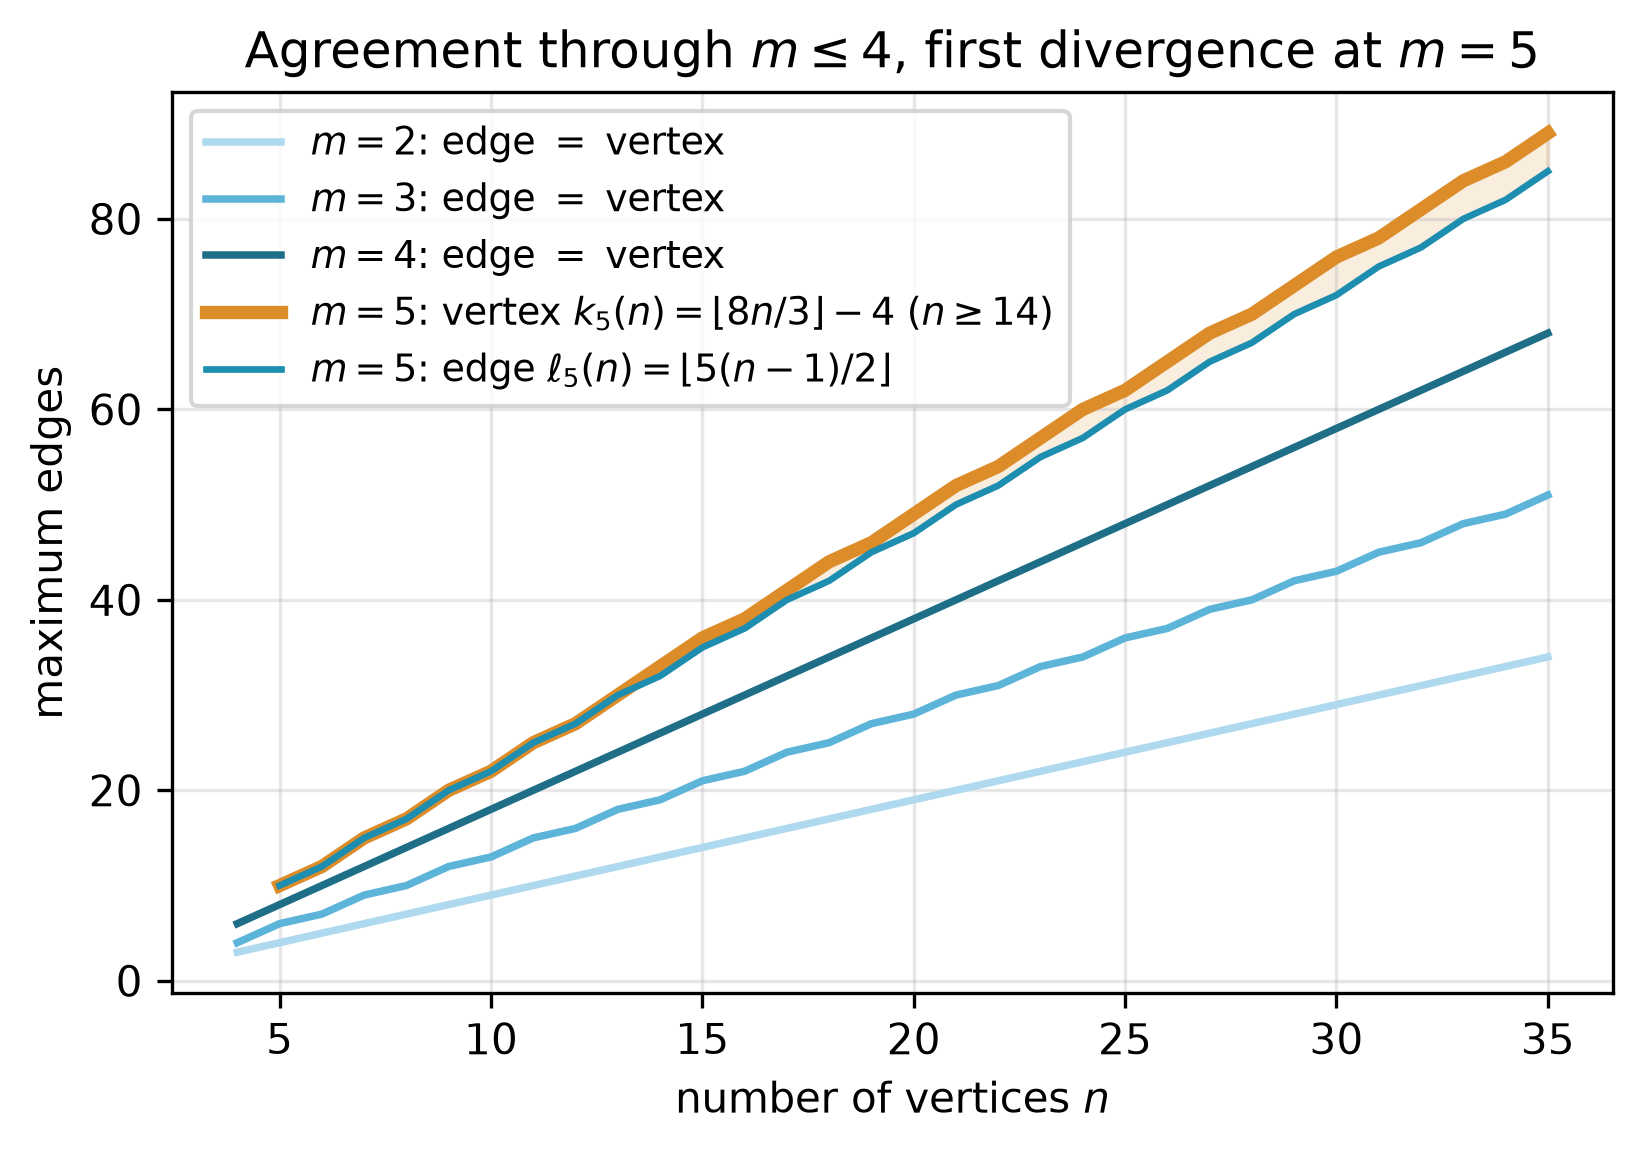
\includegraphics[width=\textwidth]{figures/edge_vertex_divergence.png}
    \caption{The edge and vertex extremal functions for $m = 2, 3, 4$ (blue shades, single curve per $m$ since they agree) and $m = 5$ (thin blue for edge, thick orange for vertex). The vertex function diverges from the edge function at $n = 14$ and grows faster thereafter.}
    \label{fig:divergence}
\end{figure}

\subsection{Directed graphs at the first threshold}

\begin{theorem}[Directed arc value at $m = 2$]\label{thm:dir-arc-m2-exact}
For simple digraphs,
\[
    \ell_2^{\mathrm{dir}}(n) = \max\!\left(2(n-1),\ \floorfrac{n^2}{4}\right).
\]
\end{theorem}

Two constructions attain the two terms (\Cref{fig:simple-digraph-m2}).
The bidirected star has $2(n-1)$ arcs.
The one-way complete bipartite digraph has all arcs from one half of the vertices to the other half, so it has $\floor{n^2/4}$ arcs.
In both, every ordered pair is joined by at most one directed path.
\Cref{sec:dir-constructions} gives the details.

For the upper bound we use a \emph{reachability skeleton}: a subdigraph in which $u$ can reach $v$ exactly when $u$ can reach $v$ in the whole digraph.
\Cref{lem:reach-skeleton} shows that there is always a skeleton with at most $M(n)=\max(2(n-1),\floor{n^2/4})$ arcs.
At $m=2$, an arc outside the skeleton would give a second route between its ends.
So a feasible digraph is its own skeleton.
This proves the bound for vertex separation, and so also for arc separation (\Cref{sec:dir-arc-m2}).

\begin{theorem}[Directed vertex value at $m = 2$]\label{thm:dir-vertex-m2-exact}
For simple digraphs, $k_2^{\mathrm{dir}}(n) = \ell_2^{\mathrm{dir}}(n)$.
\end{theorem}

\begin{figure}[ht]
\centering
\begin{tikzpicture}[>=Stealth, scale=1.0,
    smallleftvertex/.style={gvertex}, smallrightvertex/.style={gvsink},
    hubvertex/.style={gvhub}, leftvertex/.style={gvertex},
    arc/.style={gdir},
    carc/.style={gdir, vertexorange!80!black}]

  % --- left panel: the bidirected star at n = 7, hub plus six spokes = 12 arcs ---
  \begin{scope}[shift={(-5.4,1.0)}, scale=0.92]
    \node[hubvertex, minimum size=7mm] (h) at (0,0) {$h$};
    \foreach \i/\ang in {0/90, 1/150, 2/210, 3/270, 4/330, 5/30} {
      \node[leftvertex, minimum size=7mm] (v\i) at (\ang:2.2) {$\i$};
    }
    \foreach \i in {0,...,5} {
      \draw[arc] (h) to[bend left=13] (v\i);
      \draw[arc] (v\i) to[bend left=13] (h);
    }
  \end{scope}
  % --- right panel: B_{3,4} at n = 7, every A-to-B arc = 12 arcs ---
  \begin{scope}[on background layer]
    \node[draw=KULblauw1!25, fill=KULblauw1!6, rounded corners=10pt,
          fit={(0,-0.6) (0,2.6)}, inner sep=8pt, minimum width=12pt] {};
    \node[draw=vertexred!25, fill=vertexred!6, rounded corners=10pt,
          fit={(4,-0.6) (4,2.6)}, inner sep=8pt, minimum width=12pt] {};
  \end{scope}
  \foreach \i in {1,...,3} {
    \node[smallleftvertex]  (a\i) at (0, {2.0-1.0*(\i-1)}) {$a_{\i}$};
  }
  \foreach \j in {1,...,4} {
    \node[smallrightvertex] (b\j) at (4, {2.5-1.0*(\j-1)}) {$b_{\j}$};
  }
  \foreach \i in {1,...,3} {
    \foreach \j in {1,...,4} {
      \draw[arc] (a\i) -- (b\j);
    }
  }
  \node[font=\small] at (0,-1.3) {$A$};
  \node[font=\small] at (4,-1.3) {$B$};
\end{tikzpicture}
\caption{The two branches tie at $n=7$, where each holds $12$ arcs at $\lec^{\max}=1$. Left: the bidirected star, a hub joined to six spokes both ways, $2(n-1)=12$. Right: the one-directional complete bipartite digraph $B_{3,4}$, every arc from $A$ to $B$, $\floor{n^2/4}=12$.}
\label{fig:simple-digraph-m2}
\end{figure}

The star has more arcs for $n<7$, and the bipartite digraph has more for $n>7$.
So the directed value grows quadratically in $n$, while the undirected value grows linearly.
The reason is that all arcs can point the same way, so no route comes back.

\subsection{Undirected hypergraphs}

\begin{theorem}[Hypergraph edge bound]\label{prop:hyper-edge}
For $n\ge r\ge2$ and $m\ge2$, an $r$-uniform multihypergraph on $n$ vertices with $\lec^{\max}\le m-1$ has size at most $\floorfrac{(m-1)(n-1)}{r-1}$. There are simple hypergraphs attaining the bound when $m - 1 \le \binom{n-2}{r-2}$, and multihypergraphs attaining it when $(r-1) \mid n - 1$.
\end{theorem}

\Cref{app:proofs} proves the bound by induction on $n$: it cuts the hypergraph into two parts.
The star hypertree of \Cref{fig:hyper-star} attains the bound at $m=2$.
It has a hub joined to disjoint groups of $r-1$ vertices.
For $r\ge3$, simple hypergraphs attain the bound whenever $m-1\le\binom{n-2}{r-2}$ (\Cref{thm:simple-hyper-edge}).
So for $r\ge3$, unlike for graphs, repeated edges often do not help.
The condition says that there are enough different hyperedges.
When it fails, the simple value can be smaller.
For example, at $n=r=m=3$ there is only one possible hyperedge.
A simple hypergraph has one hyperedge, while a multihypergraph can have two copies of it (\Cref{rem:simple-hyper-necessary}).

\begin{figure}[ht]
\centering
\begin{tikzpicture}[scale=1.0,
   stn/.style={metrostop, minimum size=6mm},
   hub/.style={metrostop, minimum size=8.5mm, draw=vertexorange!90!black,
               fill=vertexorange!45, line width=1.4pt}]
  \coordinate (h) at (0,0);
  % two horizontal rows of four stations, the hub centred between them
  \coordinate (i1) at (-0.95, 1.3);  \coordinate (o1) at (-2.65, 1.3);
  \coordinate (i2) at ( 0.95, 1.3);  \coordinate (o2) at ( 2.65, 1.3);
  \coordinate (i3) at (-0.95,-1.3);  \coordinate (o3) at (-2.65,-1.3);
  \coordinate (i4) at ( 0.95,-1.3);  \coordinate (o4) at ( 2.65,-1.3);
  \begin{scope}[on background layer]
    % each hyperedge is one metro line: hub --(diagonal)-- inner --(horizontal)-- outer
    \draw[metro, metroA] (h) -- (i1) -- (o1);
    \draw[metro, metroB] (h) -- (i2) -- (o2);
    \draw[metro, metroC] (h) -- (i3) -- (o3);
    \draw[metro, metroD] (h) -- (i4) -- (o4);
  \end{scope}
  \foreach \p in {i1,o1,i2,o2,i3,o3,i4,o4} {\node[stn] at (\p) {};}
  \node[hub] at (h) {$h$};
\end{tikzpicture}
\caption{The $r=3$, $n=9$ star hypertree: four hyperedges meet only at the hub $h$, attaining $\floor{(n-1)/(r-1)}=4$ with $\lec^{\max}=1$.}
\label{fig:hyper-star}
\end{figure}

\begin{theorem}[Hypergraph vertex value at $m = 2$]\label{thm:hyper-vertex-m2}
For $r \ge 2$ and $n \ge 1$, the maximum number of hyperedges of an
$r$-uniform multihypergraph on $n$ vertices with $\kap^{\max} \le 1$ is
\[
    K_2^{(r)}(n) \;=\; \floorfrac{n-1}{r-1},
\]
attained by the star hypertree of \Cref{fig:hyper-star}, which is simple. In
particular $K_2^{(r)}(n) = k_2^{(r)}(n) = \ell_2^{(r)}(n)$: the vertex and edge
problems agree at $m = 2$ for every uniformity, and repeated hyperedges never
help.
\end{theorem}

\begin{theorem}[Hypergraph vertex value at $m = 3$]\label{thm:hyper-vertex-m3}
For $r \ge 2$ and $n\ge1$, every $r$-uniform multihypergraph on $n$ vertices with
$\kap^{\max} \le 2$ has at most $\floorfrac{2(n-1)}{r-1}$ hyperedges. For
$2 < r < n$, which is exactly the range where $2 \le \binom{n-2}{r-2}$, the bound
is attained by a simple hypergraph, so
\[
    k_3^{(r)}(n) \;=\; \floorfrac{2(n-1)}{r-1} \;=\; \ell_3^{(r)}(n).
\]
When $(r-1) \mid (n-1)$, a multihypergraph attains it, so then
$K_3^{(r)}(n) = \floor{2(n-1)/(r-1)}$
(\Cref{prop:hyper-vertex-lower-multi}).
\end{theorem}

Both proofs use the incidence graph (\Cref{sec:hyper-vertex-proof}).
At $m=3$ the proof bounds the number of independent cycles of the incidence graph.
We have no such bound for $m\ge4$.



For $r=2$ these results are about multigraphs.
They give $K_2(n)=n-1$, attained by trees, and $K_3(n)=2(n-1)$, attained by a tree with every edge doubled (\Cref{cor:multi-vertex-m3}).
For $m=5$ the vertex and edge values differ: the thickened theta of \Cref{sec:multi-vertex} gives $K_5(4)\ge14$, while $L_5(4)=12$.
For $m=4$ this is open.
\Cref{sec:multi-vertex} discusses larger $m$.

\subsection{Directed bounds beyond the first threshold}

\begin{theorem}[The quadratic bound with a linear error]\label{thm:dir-arc-linear-error}
For all $m \ge 2$ and $n \ge 2$, every simple digraph $D$ on $n$ vertices with $\lec^{\max}_D \le m-1$, or with $\kap^{\max}_D \le m-1$, satisfies
\[
    |A(D)| \;\le\; \floorfrac{n^2}{4} \;+\; 4(m-1)(n-1),
\]
so for each fixed $m$,
\[
    \ell_m^{\mathrm{dir}}(n) \;=\; \frac{n^2}{4} \;+\; \Theta_m(n) \quad\text{and}\quad k_m^{\mathrm{dir}}(n) \;=\; \frac{n^2}{4} \;+\; \Theta_m(n) \qquad (m\ge3)\text{.}
\]
\end{theorem}


\Cref{app:proofs} gives the proof. It counts routes of length two.
For an ordered pair $(u,v)$, the routes $u\to x\to v$ with different midpoints $x$, together with the arc $u\to v$, are disjoint.
So a feasible digraph has at most $m-1$ of them.
Summing over all pairs bounds $\sum_x d^+(x)\,d^-(x)$.
The proof is by induction on $n$.
If some vertex has total degree below $n/2$, we delete it and use the bound on $n-1$ vertices.
Otherwise every total degree is at least $n/2$, and the sum above makes $\sum_x \min(d^+(x),d^-(x))$ at most linear in $n$.
At every vertex we then delete its in-arcs or its out-arcs, whichever are fewer.
These deleted arcs give the linear term.
What remains has all arcs from one part to the other, so it has at most $\floor{n^2/4}$ arcs.
The routes of length two are also internally vertex-disjoint, so the same proof works for vertex separation.


\begin{theorem}[Directed multigraph value, every $n$ and $m$]\label{thm:dir-multi-full}
For all $n \ge 2$ and $m \ge 2$,
\[
    L_m^{\mathrm{dir}}(n) \;=\; (m-1)\,M(n), \qquad M(n) := \max\!\Bigl(2(n-1),\ \floorfrac{n^2}{4}\Bigr).
\]
\end{theorem}

The bound is attained in two ways: by a bidirected tree with every arc taken $m-1$ times, and by the one-way complete bipartite digraph with every arc taken $m-1$ times.
The proof works as follows.
Every feasible multigraph contains a small reachability skeleton.
Removing one copy of each skeleton arc lowers $\lec(u,v)$ by at least one for every pair with $\lec(u,v)>0$.
So $m-1$ such removals remove all arcs.
For $n\ge\max(8,2m)$ the bipartite construction is the only extremal multigraph, up to reversing all arcs (\Cref{thm:dir-multi-uniqueness}).

A directed hyperedge is \emph{forward} if it has one tail and $r-1$ heads, as above.

\begin{theorem}[The directed hypergraph constant]\label{thm:dir-hyper-constant}
Let $r \ge 2$ and $m \ge 2$. Every forward directed $r$-uniform multihypergraph
$\HH$ on $n \ge 2$ vertices with $\kap^{\max}_{\HH} \le m-1$ satisfies
\[
    |E(\HH)| \;\le\; \frac{m-1}{r-1}\floorfrac{n^2}{4} \;+\; 4(m-1)^2 (n-1).
\]

\end{theorem}

Since $\kap\le\lec$, the same bound holds when $\lec^{\max}_\HH\le m-1$. The construction of \Cref{prop:dir-hyper-first} has $(1+o(1))(m-1)n^2/(4(r-1))$ hyperedges, so the leading term is right.

\Cref{app:proofs} gives the proof.
It uses the \emph{shadow} digraph, which has an arc $u\to v$ when some hyperedge has tail $u$ and head $v$.
Each hyperedge gives $r-1$ arcs of the shadow, and each arc comes from at most $m-1$ hyperedges.
The route condition on the hypergraph limits the routes of length two in the shadow.
\Cref{lem:two-step-budget} then bounds the number of arcs of the shadow.

At $r=2$ this also covers directed multigraphs with vertex separation.
At $m=2$ no arc can be repeated, so $K_2^{\mathrm{dir}}(n)=\ell_2^{\mathrm{dir}}(n)$.
For fixed $m$, the extremal multigraphs of \Cref{thm:dir-multi-full} are feasible here too, since $\kap\le\lec$.
With \Cref{thm:dir-hyper-constant} at $r=2$ this gives $K_m^{\mathrm{dir}}(n)=(m-1)n^2/4+O_m(n)$ (\Cref{cor:dir-multi-incidence}).

\Cref{sec:status-simple-directed} compares this with a theorem of Huang and Lyu \cite{HuangLyu26}.


\chapter{Measuring and Searching by Machine}
\label{ch:machine}\label{ch:certify}\label{ch:discover}
% !TEX root = ../main.tex

Chapter~1 stated the problem and the proved results.
This chapter explains how a program can measure connectivity in every variant, check small graphs one by one, and search for dense examples.
No result in this thesis depends on the output of this program.
Its output for $n,m\le7$ is printed in \Cref{app:program}.
\Cref{sec:certificates} shows how an output can be checked without reading the code.

The program is one Python file of about $750$ lines, \texttt{program/erdos915.py}.
It uses the library \texttt{networkx} for maximum flows, and the programs \texttt{geng}, \texttt{directg} and \texttt{genbg} of \texttt{nauty} to list graphs.
This chapter prints the main parts of the program, each next to the idea it implements.
The remaining parts, such as the imports and small helper functions, are in \Cref{app:program}, so every line of the program is printed once.
The names in the code follow the words of the text.
\Cref{fig:spine} shows the structure of the program.
\begin{figure}[ht]
\centering
\spinediagram
\caption{One model feeds the max-flow computation. Exhaustive search uses it to find exact values, heuristic search uses it to find dense examples, and the check with \texttt{nauty} uses it to show that no feasible graph has one edge more than the densest one found (\Cref{sec:one-more}).}
\label{fig:spine}
\end{figure}

\section{Modelling}
The program treats all eight models in one way.
A model is described by four facts: whether it is directed, whether edges may repeat, the edge size $r$, and, for directed hypergraphs, the allowed numbers of tails.
A graph is the case $r=2$.
The program runs each directed hypergraph model in three versions, forward, backward and general (\Cref{sec:variants}), so \texttt{ALL\_MODELS} lists twelve entries for the eight models.
The separation, edge or vertex, is a separate choice, so the eight models give the sixteen problems.
A \texttt{Problem} bundles a model, a separation, the number of vertices $n$ and the threshold $m$, and every function below takes one (\Cref{lst:models}).

\programpart{models}{The models, with three versions of each directed hypergraph model, and the two separations.}

Every edge is stored as a hyperedge: its vertices, and its tails if the model is directed.
An ordinary edge $uv$ is the hyperedge $\{u,v\}$ without tails, and an arc $u\to v$ is the hyperedge $\{u,v\}$ with tail $u$.
A route may enter a hyperedge only at one of its \emph{entry vertices}, and leave it only at one of its \emph{exit vertices} (\texttt{entry\_vertices} and \texttt{exit\_vertices} in the code).
In an undirected hyperedge every vertex is both. In a directed one only the tails are entries and only the heads are exits.
A candidate graph is a table that gives every possible hyperedge its multiplicity.
We call the models without repeated edges \emph{simple models}, and the models with repeated edges \emph{multi models}.
In a simple model every multiplicity is $0$ or $1$. In a multi model it is at most $m-1$, since $m$ copies of one edge already give $m$ disjoint routes (\Cref{lst:hyperedges}).
\Cref{fig:matrix-rep} shows two such tables.

\programpart{hyperedges}{Hyperedges, the list of all possible hyperedges, and the largest useful multiplicity.}



\begin{figure}[ht]
\centering
\newcommand{\hetable}[1]{%
  {\small\renewcommand{\arraystretch}{1.15}%
  \begin{tabular}{@{}ccc@{}}
  \texttt{\color{codeConstant}TAILS} & \texttt{\color{codeConstant}MEMBERS} & copies\\ \midrule
  #1
  \end{tabular}}}
\begin{tikzpicture}[>=Stealth]
% ---- (a) directed multigraph -> its hyperedge table ----
\node[vertex] (A) at (0,   0)   {$1$};
\node[vertex] (B) at (2.0, 0)   {$2$};
\node[vertex] (C) at (1.0, 1.7) {$3$};
\draw[arc] (A) to[bend left=15]  (B);
\draw[arc] (A) to[bend right=15] (B);
\draw[arc] (B) to[bend left=15]  (C);
\draw[arc] (C) to[bend left=15] (B);
\draw[arc] (A) -- (C);
\node[font=\small] at (1.0, -0.8) {directed multigraph};
\node at (3.4, 0.55) {$\longrightarrow$};
\node at (6.2, 0.55) {\hetable{
  $\{1\}$ & $\{1,2\}$ & ${\color{vertexred}\mathbf 2}$ \\
  $\{1\}$ & $\{1,3\}$ & $1$ \\
  $\{2\}$ & $\{2,3\}$ & $1$ \\
  $\{3\}$ & $\{2,3\}$ & $1$ \\}};
\node[font=\small] at (1.0, -1.25) {(a)};
% ---- (b) directed hypergraph -> its hyperedge table ----
\begin{scope}[yshift=-3.9cm]
  \coordinate (p1) at (0.0, 0.6);
  \coordinate (p2) at (0.0,-0.6);
  \coordinate (p3) at (1.1, 0.0);
  \coordinate (p4) at (2.2, 0.6);
  \coordinate (p5) at (2.2,-0.6);
  \begin{scope}[on background layer]
    \draw[metro, metroA, -{Stealth[length=2.6mm]}, shorten >=2mm, shorten <=1.4mm] (p3) -- (p1);
    \draw[metro, metroA, -{Stealth[length=2.6mm]}, shorten >=2mm, shorten <=1.4mm] (p3) -- (p2);
    \draw[metro, metroB, -{Stealth[length=2.6mm]}, shorten >=2mm, shorten <=1.4mm] (p3) -- (p5);
    \draw[metro, metroB, -{Stealth[length=2.6mm]}, shorten >=2mm, shorten <=1.4mm] (p4) -- (p5);
  \end{scope}
  \foreach \p/\lbl in {p1/1,p2/2,p3/3,p4/4,p5/5} {\node[smallvertex] at (\p) {$\lbl$};}
  \node[font=\small] at (1.1,-1.15) {directed hypergraph};
  \node at (3.4, 0.0) {$\longrightarrow$};
  \node at (6.2, 0.0) {\hetable{
    {\color{metroA}$\{\mathbf 3\}$} & {\color{metroA}$\{1,2,3\}$} & $1$ \\
    {\color{metroB}$\{\mathbf 3,\mathbf 4\}$} & {\color{metroB}$\{3,4,5\}$} & $1$ \\}};
  \node[font=\small] at (1.1,-1.6) {(b)};
\end{scope}
\end{tikzpicture}
\caption{The program stores every model in one way: a table that gives each hyperedge its number of copies. (a) A directed multigraph. The arc $u\to v$ is the hyperedge with members $\{u,v\}$ and tail $u$, and the two parallel arcs from $1$ to $2$ are one row with $2$ copies. (b) A directed $3$-uniform hypergraph in the general model. Each hyperedge records its tails and its three members: the red one has tail $3$, the blue one has tails $3$ and $4$ and head $5$. In an undirected model there are no tails. A hyperedge that does not occur has $0$ copies and is left out.}
\label{fig:matrix-rep}
\end{figure}

\section{Measuring}
Every search below needs $\lec^{\max}$ or $\kap^{\max}$ of a candidate graph.
This section explains how the program computes them.

To compute $\lec(u,v)$ we use a maximum flow.
In a network every link has a capacity, and a \emph{maximum flow} is the largest amount that can be sent from $u$ to $v$.
We give each pair of vertices a link with capacity $\mu(u,v)$.
In a digraph the link has a direction. In an undirected graph it can be used in both directions.
The max-flow min-cut theorem of Ford and Fulkerson \cite{FordFulkerson56} says that the maximum flow equals the smallest capacity of a cut.
By Menger's theorem, this is $\lec(u,v)$.
So computing a maximum flow computes $\lec(u,v)$.
We call this the \emph{max-flow computation}.


\subsection{Transformations}
The max-flow computation works on one kind of network for all sixteen problems.

Every hyperedge, including an ordinary edge, becomes a \emph{gate} (\Cref{fig:hyper-gadget}).
The gate has an entry node and an exit node, joined by one arc whose capacity is the multiplicity of the hyperedge.
Each vertex of the hyperedge gets an arc of unlimited capacity to the entry node and one from the exit node.
So the arc inside the gate is the only bottleneck.
For a directed hyperedge, only the tails have an arc to the entry, and only the heads have an arc from the exit (\Cref{fig:dir-hyper-gadget}).
So a route must go from a tail to a head.
\Cref{thm:menger-hyper} shows that the maximum flow in this network is the number of hyperedge-disjoint Berge routes.
\Cref{fig:hyper-gadget-example} shows an example.

Every vertex $v$ is split into two nodes $v^{\mathrm{in}}$ and $v^{\mathrm{out}}$, joined by one arc (\Cref{fig:vertex-split}).
Routes arrive at $v^{\mathrm{in}}$ and leave from $v^{\mathrm{out}}$.
For vertex separation this arc has capacity one, so at most one route can pass through $v$.
For edge separation its capacity is unlimited, and it changes nothing.
The gates keep their capacity, so parallel copies still give separate routes, as in the incidence convention of \Cref{sec:incidence-convention}.
\Cref{lst:network} builds this network.

\programpart{network}{The flow network: split vertices and one gate per hyperedge.}

The number of disjoint routes from $u$ to $v$ is the maximum flow from $u^{\mathrm{out}}$ to $v^{\mathrm{in}}$ (\Cref{lst:measure}).
A graph is feasible when this number is below $m$ for every pair, ordered in directed models.
The flow may stop as soon as it reaches $m$, since a larger value changes nothing. This is the \texttt{stop\_at} argument.

\programpart{measure}{Counting disjoint routes, and the feasibility test.}

\begin{figure}[htbp]
\centering
% Printed legibility: this picture holds two 8-unit panels side by side, so
% every extra centimetre of gap or of resize headroom is paid for twice over in
% label size. The gap is kept tight, the box is given the full text width, and
% the station and gate fonts are stepped up, which together lift the smallest
% label from about 5.4pt to roughly 9pt on paper.
\resizebox{\textwidth}{!}{%
\begin{tikzpicture}[scale=0.92, >=Stealth,
   metro/.append style={line width=3.0pt},
   metrostop/.append style={font=\small\bfseries, minimum size=6.6mm},
   faded/.style={metro, opacity=0.35, line width=2.2pt},
   flow/.style={line width=1.2pt, black!88, line cap=round,
                preaction={draw, line width=3.0pt, white}},
   gate/.style={circle, fill=white, draw=black!30, line width=0.6pt,
                inner sep=0.4pt, minimum size=13.5pt, font=\small}]
\def\stations{%
  \coordinate (Sa) at (0,0);  \coordinate (Sc) at (2,2);  \coordinate (Sd) at (6,2);
  \coordinate (Se) at (0,4);  \coordinate (Sj) at (8,4);  \coordinate (Sl) at (2,6);
  \coordinate (Sm) at (6,6);  \coordinate (Sn) at (0,8);}
% Every station carries its own letter, since the captions name hyperedges and
% routes by those letters.  The chosen pair also carries its role name, u or v,
% in blue just outside the station.
\def\drawstops{%
  \foreach \id/\lab in {Sa/a,Sc/c,Sd/d,Se/e,Sj/j,Sl/l,Sm/m,Sn/n}
     {\node[metrostop] at (\id) {$\lab$};}
  \node[font=\small\bfseries, text=KULblauw1] at ($(Se)+(-0.62,0.52)$) {$u$};
  \node[font=\small\bfseries, text=KULblauw1] at ($(Sm)+(0.62,0.52)$) {$v$};}
% --- panel (a): the hypergraph, every hyperedge vertex to vertex ---
\begin{scope}
  \stations
  \begin{scope}[on background layer]
    \draw[metro, metroA] (Se) -- (Sa);
    \draw[metro, metroA] (Sa) -- (Sd);
    \draw[metro, metroB] (Sn) -- (Sm);
    \draw[metro, metroB] (Sm) -- (Sj);
    \draw[metro, metroC] ($(Se)+(0.14,-0.14)$) -- ($(Sl)+(0.14,-0.14)$);
    \draw[metro, metroC] (Sl) -- (Sc);
    \draw[metro, metroD] (Se) -- (Sd);
    \draw[metro, metroD] (Sd) -- (Sm);
    \draw[metro, metroF] (Sn) -- (Se);
    \draw[metro, metroF] (Se) -- (Sl);
    \draw[metro, metroH] ($(Se)+(-0.14,0.14)$) -- ($(Sl)+(-0.14,0.14)$);
    \draw[metro, metroH] (Sl) -- (Sm);
    \draw[metro, metroG] (Sm) -- (Sc);
    \draw[metro, metroG] (Sc) -- (Sj);
    \draw[metro, metroE] (Sl) -- (Sd);
    \draw[metro, metroE] (Sd) -- (Sj);
  \end{scope}
  \drawstops
  \node[font=\small] at (4,-1.4) {(a)};
\end{scope}
% --- panel (b): the helper-point flow network for the pair u, v ---
\begin{scope}[xshift=9.6cm]
  \stations
  \coordinate (Helc) at (1,3);
  \coordinate (Hmcj) at (5,4);
  \coordinate (Hedm) at (3,3.7);
  \coordinate (Helm) at (1.6,6.7);
  \coordinate (Hnel) at (0.50,6.00);
  \coordinate (Hnmj) at (3.27,7.81);
  \begin{scope}[on background layer]
    \draw[faded, metroA] (Se) -- (Sa);
    \draw[faded, metroA] (Sa) -- (Sd);
    \draw[faded, metroB] (Sn) -- (Sm);
    \draw[faded, metroB] (Sm) -- (Sj);
    \draw[faded, metroC] ($(Se)+(0.14,-0.14)$) -- ($(Sl)+(0.14,-0.14)$);
    \draw[faded, metroC] (Sl) -- (Sc);
    \draw[faded, metroD] (Se) -- (Sd);
    \draw[faded, metroD] (Sd) -- (Sm);
    \draw[faded, metroF] (Sn) -- (Se);
    \draw[faded, metroF] (Se) -- (Sl);
    \draw[faded, metroH] ($(Se)+(-0.14,0.14)$) -- ($(Sl)+(-0.14,0.14)$);
    \draw[faded, metroH] (Sl) -- (Sm);
    \draw[faded, metroG] (Sm) -- (Sc);
    \draw[faded, metroG] (Sc) -- (Sj);
    \draw[faded, metroE] (Sl) -- (Sd);
    \draw[faded, metroE] (Sd) -- (Sj);
  \end{scope}
  \draw[flow] (Se) -- (Helc);
  \draw[flow] (Helc) -- (Sc);
  \draw[flow] (Sc) -- (Hmcj);
  \draw[flow] (Hmcj) -- (Sm);
  \draw[flow] (Se) -- (Hedm);
  \draw[flow] (Hedm) -- (Sm);
  \draw[flow] (Se) -- (Helm);
  \draw[flow] (Helm) -- (Sm);
  \draw[flow] (Se) -- (Hnel);
  \draw[flow] (Hnel) -- (Sn);
  \draw[flow] (Sn) -- (Hnmj);
  \draw[flow] (Hnmj) -- (Sm);
  % dotted leg from each gate to the hyperedge's unused third member
  \draw[densely dotted, line width=1pt, opacity=0.7, shorten >=3mm, metroC] (Helc) -- (Sl);
  \draw[densely dotted, line width=1pt, opacity=0.7, shorten >=3mm, metroG] (Hmcj) -- (Sj);
  \draw[densely dotted, line width=1pt, opacity=0.7, shorten >=3mm, metroD] (Hedm) -- (Sd);
  \draw[densely dotted, line width=1pt, opacity=0.7, shorten >=3mm, metroH] (Helm) -- (Sl);
  \draw[densely dotted, line width=1pt, opacity=0.7, shorten >=3mm, metroF] (Hnel) -- (Sl);
  \draw[densely dotted, line width=1pt, opacity=0.7, shorten >=3mm, metroB] (Hnmj) -- (Sj);
  \node[gate] at (Helc) {$h_{\textcolor{metroC}{\bullet}}$};
  \node[gate] at (Hmcj) {$h_{\textcolor{metroG}{\bullet}}$};
  \node[gate] at (Hedm) {$h_{\textcolor{metroD}{\bullet}}$};
  \node[gate] at (Helm) {$h_{\textcolor{metroH}{\bullet}}$};
  \node[gate] at (Hnel) {$h_{\textcolor{metroF}{\bullet}}$};
  \node[gate] at (Hnmj) {$h_{\textcolor{metroB}{\bullet}}$};
  \drawstops
  \node[font=\small] at (4,-1.4) {(b)};
\end{scope}
\end{tikzpicture}}
\caption[The gate network of a hypergraph]{(a) An undirected $3$-uniform hypergraph. (b) The relevant part of its gate network for the pair $u,v$. The four black routes use pairwise disjoint sets of gates, so $\lec(u,v)\ge4$. The vertex $v$ lies in only four hyperedges, and removing those four hyperedges separates $u$ from $v$, so $\lec(u,v)\le4$. Hence $\lec(u,v)=4$. Each gate is drawn as one point. A dotted line joins a gate to the third vertex of its hyperedge, which the route does not use.}
\label{fig:hyper-gadget-example}
\end{figure}

% Printed legibility: three panels across at 0.32\textwidth shrank each picture
% to roughly 0.58 of natural size and its labels to under 5pt. Stacking them
% one per row at 0.70\textwidth reverses that, drawing each slightly larger
% than natural instead.
\begin{figure}[ht]
\centering
\begin{subfigure}[b]{0.70\textwidth}
\centering
\resizebox{\linewidth}{!}{%
\begin{tikzpicture}[>=Stealth]
\node[vertex] (v) at (1.0, 0) {$v$};
\draw[->, edge] (0.0,  0.6) -- (v);
\draw[->, edge] (0.0, -0.6) -- (v);
\draw[->, edge] (v) -- (2.0,  0.6);
\draw[->, edge] (v) -- (2.0, -0.6);
\draw[->, very thick, color=KULblauw3b] (2.8, 0) -- (3.8, 0);
\node[smallvertex, minimum size=8mm] (vi) at (5.0, 0) {$v^{\mathrm{in}}$};
\node[smallvertex, minimum size=8mm] (vo) at (7.0, 0) {$v^{\mathrm{out}}$};
\draw[->, edge, color=KULblauw3b] (vi) -- node[above, font=\scriptsize]{capacity $1$} (vo);
\draw[->, edge] (4.0,  0.6) -- (vi);
\draw[->, edge] (4.0, -0.6) -- (vi);
\draw[->, edge] (vo) -- (8.0,  0.6);
\draw[->, edge] (vo) -- (8.0, -0.6);
\end{tikzpicture}}
\caption{Splitting each vertex $v$ into $v^{\mathrm{in}}$ and $v^{\mathrm{out}}$, joined by an arc of capacity one, turns vertex-disjoint routes into arc-disjoint routes. Only this inner arc has capacity one.}
\label{fig:vertex-split}
\end{subfigure}

\bigskip
\begin{subfigure}[b]{0.70\textwidth}
\centering
\resizebox{\linewidth}{!}{%
\begin{tikzpicture}[>=Stealth]
\coordinate (a) at (0.0, 0.0); \coordinate (b) at (1.0, 0.0); \coordinate (c) at (2.0, 0.0);
\begin{scope}[on background layer]\draw[metro, metroA] (a)--(b)--(c);\end{scope}
\node[smallvertex] at (a) {$a$}; \node[smallvertex] at (b) {$b$}; \node[smallvertex] at (c) {$c$};
\draw[->, very thick, color=KULblauw3b] (2.85, 0.0) -- (3.95, 0.0);
\begin{scope}[xshift=4.6cm]
% members in a column, gate pair beside them: every member sends one uncapped
% arc into e^- and receives one uncapped arc out of e^+.
\node[smallvertex] (a2) at (0.0,  1.30) {$a$};
\node[smallvertex] (b2) at (0.0,  0.00) {$b$};
\node[smallvertex] (c2) at (0.0, -1.30) {$c$};
\node[hnode, fill=metroA!70, minimum size=15pt] (em) at (2.05,  0.62) {$e^-$};
\node[hnode, fill=metroA!70, minimum size=15pt] (ep) at (2.05, -0.62) {$e^+$};
% into the gate
\draw[gdirfaint] (a2) to[bend left=8]  node[above, font=\scriptsize, text=black!55, pos=0.55]{$\infty$} (em);
\draw[gdirfaint] (b2) to[bend left=10] (em);
\draw[gdirfaint] (c2) to[bend left=22] (em);
% out of the gate
\draw[gdirfaint] (ep) to[bend left=22] (a2);
\draw[gdirfaint] (ep) to[bend left=10] (b2);
\draw[gdirfaint] (ep) to[bend left=8]  node[below, font=\scriptsize, text=black!55, pos=0.45]{$\infty$} (c2);
% the one bottleneck
\draw[gdir, line width=1.6pt, color=KULblauw3b] (em) -- node[right, font=\scriptsize]{capacity $\mu$} (ep);
\end{scope}
\end{tikzpicture}}
\caption{Transform a hyperedge into a gate with capacity equal to the multiplicity of the hyperedge.}
\label{fig:hyper-gadget}
\end{subfigure}

\bigskip
\begin{subfigure}[b]{0.70\textwidth}
\centering
\resizebox{\linewidth}{!}{%
\begin{tikzpicture}[>=Stealth, gatearc/.style={gdir}]
\node[smallvertex] (a) at (0.0, 1.05) {$a$}; \node[smallvertex] (b) at (-0.85, -0.55) {$b$}; \node[smallvertex] (c) at (0.85, -0.55) {$c$};
\begin{scope}[on background layer]
  \draw[metro, metroB, -{Stealth[length=2.8mm]}, shorten >=2mm, shorten <=1.4mm] (a) -- (b);
  \draw[metro, metroB, -{Stealth[length=2.8mm]}, shorten >=2mm, shorten <=1.4mm] (a) -- (c);
\end{scope}
\draw[->, very thick, color=KULblauw3b] (2.4, 0.1) -- (3.5, 0.1);
\begin{scope}[xshift=5.4cm]
  \node[smallvertex] (a2) at (0.0, 1.55) {$a$};
  \node[hnode, fill=metroB!70, minimum size=15pt] (gm) at (0.0,  0.52) {$e^-$};
  \node[hnode, fill=metroB!70, minimum size=15pt] (gp) at (0.0, -0.62) {$e^+$};
  \node[smallvertex] (b2) at (-1.05, -1.55) {$b$}; \node[smallvertex] (c2) at (1.05, -1.55) {$c$};
  \draw[gdirfaint] (a2) -- node[right, font=\scriptsize, text=black!60]{$\infty$} (gm);
  \draw[gdir, line width=1.6pt, color=KULblauw3b] (gm) -- node[right, font=\scriptsize]{capacity $\mu$} (gp);
  \draw[gdirfaint] (gp) -- node[left, pos = 0.3, font=\scriptsize, text=black!60]{$\infty$} (b2);
  \draw[gdirfaint] (gp) -- node[right, pos = 0.3, font=\scriptsize, text=black!60]{$\infty$} (c2);
\end{scope}
\end{tikzpicture}}
\caption{A directed hyperedge with one tail and two heads is transformed into a gate. This gate has capacity equal to the multiplicity of the hyperedge and every route must enter at the tail and leave at a head. With several tails, each tail has an arc to $e^-$.}
\label{fig:dir-hyper-gadget}
\end{subfigure}
\caption{The building blocks of the max-flow computation: vertex splitting, hyperedge gates and directed hyperedge gates.}
\label{fig:checker-gadgets}
\end{figure}

\section{Checking every graph with a fixed number of vertices}\label{sec:certification-standard}
The program stores a graph as a table that gives each possible hyperedge its number of copies (\Cref{fig:matrix-rep}).
The possible hyperedges depend on the model:
\begin{itemize}
\item in a graph, the $\binom n2$ pairs $\{u,v\}$,
\item in a digraph, the $n(n-1)$ ordered pairs, one for each arc $u\to v$,
\item in an $r$-uniform hypergraph, the $\binom nr$ sets of $r$ vertices, called \emph{$r$-sets},
\item in a directed $r$-uniform hypergraph, an $r$-set together with a choice of which of its vertices are tails.
A forward hyperedge has one tail, so each $r$-set gives $r$ possible hyperedges.
A backward hyperedge has one head, which also gives $r$.
In the general model the tails form any non-empty proper subset, which gives $2^r-2$.
\end{itemize}
Each entry of the table is between $0$ and the largest multiplicity: $1$ in a simple model and $m-1$ in a multi model.
To find an exact value, the program must show that no table with more copies than the best feasible graph found is feasible.
If the search stops early, it gives only a lower bound.

\begin{figure}[ht]
    \centering
    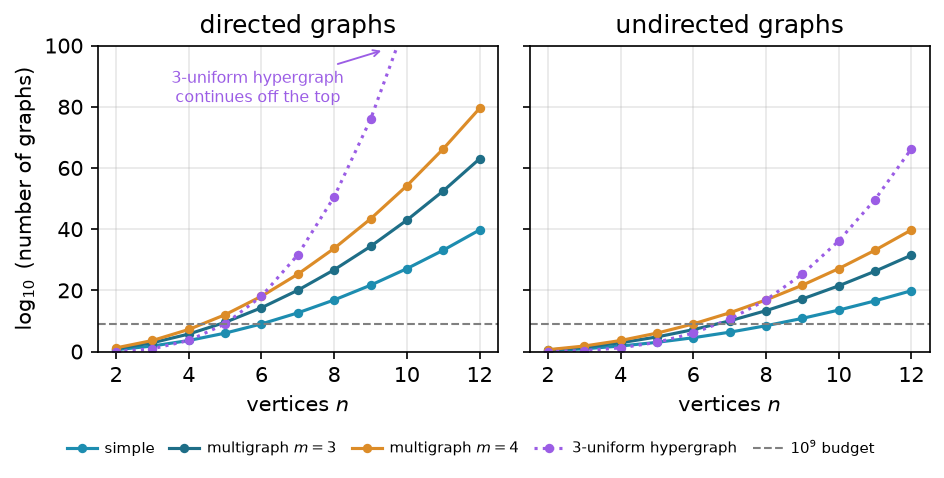
\includegraphics[width=\textwidth]{figures/complexity_growth.png}
    \caption{The number of candidates for blind enumeration, on a logarithmic scale. Every model passes $10^9$ candidates before $n=10$. Directed models grow fastest, because they have more entries to choose. The directed hypergraph curve is the forward model.}
    \label{fig:complexity}
\end{figure}

The number of vertices matters most.
The number of candidates is (values per entry) to the power (number of entries).
For graphs the number of entries grows like $n^2$, and for $r$-uniform hypergraphs like $n^r$.
A larger $m$ gives more values per entry.
Direction gives more entries, since both directions of a pair are chosen separately.
Directed hypergraphs have the most candidates, because each $r$-set carries several possible hyperedges.
The separation does not change the candidates. It only changes the test for each candidate.


So there are $2^{\binom n2}$ simple graphs and $2^{n(n-1)}$ simple digraphs on $n$ vertices.
With multiplicities at most $m-1$ there are $m^{\binom n2}$ multigraphs and $m^{n(n-1)}$ directed multigraphs.
\Cref{fig:complexity} shows how fast this grows.
The program uses two exact methods: a pruned search, for every model, and a check of the graphs with one edge more, for every model except directed hypergraphs.

\subsection{Pruned search}
A pruned search skips whole families of graphs.
Fix an order on the possible edges and decide them one at a time.
A partly built graph stands for all graphs that agree with it so far.
A pruning rule can discard this whole family.

The first rule uses that adding an edge never lowers connectivity.
If a partly built graph already breaks the condition, so does every way to complete it, and the branch is dropped.

The second rule bounds the size of every completion: the edges already placed, plus the number of undecided edges times the largest allowed multiplicity.
If this cannot beat the best graph found so far, the branch is dropped (\Cref{fig:prune}).

Both rules only drop graphs that are infeasible or cannot beat the best one.
So a finished pruned search gives the same answer as the full search.

\Cref{lst:exhaustive} decides the possible hyperedges one at a time, in a fixed order.
For each it tries $1, 2, \dots$ copies, and stops at the first number of copies that makes the graph infeasible, since more copies stay infeasible.
Then it also tries $0$ copies.
The test on \texttt{undecided} in \texttt{decide} is the second rule: if even all undecided hyperedges at full multiplicity cannot beat the best graph so far, the branch is dropped.
After the time limit the search stops and reports the best graph so far as a lower bound only.

\programpart{exhaustive}{The pruned exhaustive search.}

\begin{figure}[ht]
\centering
\begin{tikzpicture}[scale=1.0, >=Stealth,
   live/.style={gvertex, minimum size=5.5mm},
   dead/.style={gvsink, minimum size=5.5mm},
   bnd/.style={gvhub, minimum size=5.5mm},
   best/.style={gvertex, draw=vertexgreen!70!black, fill=vertexgreen!18, minimum size=5.5mm},
   br/.style={gline}]
  \node[live] (r) at (0,0) {};
  \node[live] (l) at (-2.2,-1.3) {};
  \node[live] (rr) at (2.2,-1.3) {};
  \draw[br] (r) -- node[above left, font=\scriptsize, pos=0.55]{add arc} (l);
  \draw[br] (r) -- node[above right, font=\scriptsize, pos=0.55]{skip arc} (rr);
  \node[best] (l1) at (-3.1,-2.7) {};
  \node[dead] (l2) at (-1.4,-2.7) {};
  \draw[br] (l)--(l1);
  \draw[line width=1pt, vertexred!60] (l)--(l2);
  \node[dead] (r1) at (1.3,-2.7) {};
  \node[bnd]  (r2) at (3.1,-2.7) {};
  \draw[line width=1pt, vertexred!60] (rr)--(r1);
  \draw[line width=1pt, vertexorange!70] (rr)--(r2);
  \node[font=\scriptsize, vertexgreen!50!black, align=center] at (-3.1,-3.5) {best\\feasible};
  \node[font=\scriptsize, vertexred, align=center] at (-1.4,-3.5) {infeasible\\(prune)};
  \node[font=\scriptsize, vertexred, align=center] at (1.3,-3.5) {infeasible\\(prune)};
  \node[font=\scriptsize, vertexorange!80!black, align=center] at (3.1,-3.5) {cannot beat\\best (prune)};
\end{tikzpicture}
\caption{Each level of the search decides one arc. Partly built graphs that are already infeasible (red), and branches that cannot beat the best graph found so far (orange), are dropped.}
\label{fig:prune}
\end{figure}

\subsection{Checking one edge more}\label{sec:one-more}
The pruned search meets every graph many times.
Renaming the vertices of a graph gives a graph with the same number of edges and the same connectivities, so the renamed graph is feasible exactly when the original is.
A graph on $n$ vertices has up to $n!$ renamings, so most of the work of the pruned search repeats work it has already done.

The second method avoids this.
It starts from a feasible graph with $L$ edges, found by the pruned search or by the heuristic search of \Cref{sec:heuristic}.
Removing an edge creates no new route, so it never makes a feasible graph infeasible.
So if a feasible graph with more than $L$ edges existed, removing edges from it one at a time would give a feasible graph with exactly $L+1$ edges.
It is therefore enough to check every graph with exactly $L+1$ edges.
If none of them is feasible, $L$ is the maximum.
If one of them is feasible, the program keeps it, replaces $L$ by $L+1$, and checks again.

To list these graphs, each only once up to renaming the vertices, the program uses the toolkit \texttt{nauty} of McKay and Piperno \cite{McKayPiperno14}, to which Prof.\ Jan Goedgebeur pointed us.
Three of its programs cover six of the eight models:
\begin{itemize}
\item \texttt{geng} lists the simple graphs on $n$ vertices with a given number of edges,
\item \texttt{directg} takes each graph from \texttt{geng} and directs each of its edges one way or both ways, which lists the simple digraphs,
\item \texttt{genbg} lists bipartite graphs: graphs whose vertices are split into two sides, with every edge joining the two sides. A hypergraph is the bipartite graph with the $n$ vertices on one side and the hyperedges on the other side, each hyperedge joined to its $r$ vertices. With the option \texttt{-z} no two hyperedges have the same vertices, so the hypergraph is simple.
\end{itemize}
\texttt{nauty} has no program that lists directed hypergraphs, so the program does not run this check for them. Their exact values come from the pruned search only.

\texttt{nauty} lists simple graphs only.
The \emph{support} of a multigraph is the simple graph of the pairs, or $r$-sets, that carry at least one copy.
For a multi model the program takes each support from \texttt{nauty} and chooses the number of copies of each of its edges, between $1$ and $m-1$, with $L+1$ copies in total.
A support with $k$ edges carries between $k$ and $k(m-1)$ copies, so only supports with between $\lceil (L+1)/(m-1)\rceil$ and $L+1$ edges are listed.
Renaming the vertices of a multigraph renames its support in the same way, so every multigraph with $L+1$ edges arises from some listed support.
Two choices of copies on the same support can give the same multigraph up to renaming. This repeats work but does not affect the result.
In a simple model the support is the graph itself, with one copy of each edge.
The copies are chosen one edge at a time, as in the pruned search: the program tries $1, 2, \dots$ copies and stops at the first number that makes the graph infeasible, since more copies stay infeasible.

\Cref{lst:nauty} builds the \texttt{nauty} commands and reads their output one support at a time, so the check can stop at its time limit before all supports are listed.
For digraphs two programs work together: \texttt{geng} passes every graph it lists to \texttt{directg}, which directs its edges.
The program counts the list as complete only if both programs exit normally.
If \texttt{geng} failed and \texttt{directg} did not, \texttt{directg} would receive no graphs and exit normally. The list would then look empty, and the check would report a value as exact without having checked anything.
\Cref{lst:larger} chooses the copies, and repeats the check while it finds a feasible graph with one edge more.

\programpart{nauty}{Listing the supports with \texttt{geng}, \texttt{directg} and \texttt{genbg} from \texttt{nauty}.}

\programpart{larger}{Checking every graph with one edge more.}

\section{The heuristic search}\label{sec:heuristic}
For larger $n$ the full search is impossible.
Instead we search for dense graphs in a guided way.
A \emph{heuristic} is a rule that moves the search towards better graphs.
The methods below also allow moves that make the graph worse, so that the search does not get stuck.

For graphs and digraphs, each candidate gets an \emph{energy}
\[
    \Phi(G) = -|E(G)| + \Lambda \cdot \max\bigl(0,\ c^{\max}(G) - (m - 1)\bigr).
\]
Here $c^{\max}(G)$ is $\lec^{\max}(G)$ or $\kap^{\max}(G)$, depending on the separation, and $\Lambda>0$ is a fixed penalty.
Low energy means many edges and no excess connectivity.
In the program $\Lambda$ is \texttt{PENALTY\_PER\_EXCESS\_ROUTE} (\Cref{lst:energy}).

\programpart{energy}{The energy of a candidate graph.}

The search starts from the empty graph and changes one multiplicity by one at each step.
We use \emph{tabu search} \cite{Glover89}.
At each step it makes the best allowed move, even if every move raises the energy.
After a move, the changed pair is \emph{tabu} for a fixed number of steps, so the search cannot undo the move at once.
A move that gives a better graph than any seen so far is always allowed.
When the search stalls, it makes a small change to escape: it removes all copies of three random hyperedges.
\Cref{lst:neighbours} lists the moves, and \Cref{lst:tabu} is the search itself.
The search keeps the exact connectivity of every pair of the current graph in \texttt{connectivity}, and \texttt{highest\_after} uses it to judge a move cheaply (\Cref{sec:near-cap}).

\programpart{neighbours}{The moves: one copy more or one copy less of one hyperedge.}

\programpart{tabu}{Tabu search.}

The program also implements simulated annealing on the same energy.
It accepts a worse move with a probability that decreases over time.
At temperature $T$ a move that raises the energy by $\Delta$ is accepted with probability $e^{-\Delta/T}$, and $T$ shrinks by a fixed factor at every step.
The driver in \Cref{lst:driver} does not use it, so its code is in \Cref{app:program} (\Cref{lst:annealing}).

Every feasible graph can be built from the empty graph by adding edges one at a time, staying feasible.
Still, it can help to pass through infeasible graphs: exchanging two edges may need an extra edge first.
Tabu search allows this, but it only keeps feasible results.

Each search keeps the densest feasible graph it has seen.

\subsection{Random greedy growth for hypergraphs}

For hypergraphs we use random greedy growth.
Each run starts with the empty hypergraph and a shuffled list of all possible hyperedges: each hyperedge once in the simple model, and $m-1$ times in the multi model.
The procedure adds the hyperedges one by one, and keeps each one only if the hypergraph stays feasible.
This is repeated with new random orders, and the densest result is kept.

At the end of a run no single hyperedge can be added, because a rejected hyperedge stays infeasible when more hyperedges are added.
This does not mean the result is as large as possible: an early choice can block several later ones.
We use this method instead of tabu search because there are many possible hyperedges, for example $\binom nr$ in the undirected simple case.

\programpart{greedy}{Random greedy growth.}

\subsection{Measuring only when needed}\label{sec:near-cap}
A move adds or removes one copy of one hyperedge.
Removing a copy never raises a connectivity, since every route of the smaller graph is also a route of the larger one.
Adding a copy raises $\lec(u,v)$ and $\kap(u,v)$ by at most one for every pair.
To see this, take a largest family of disjoint $u$--$v$ routes after the addition.
In the incidence convention of \Cref{sec:incidence-convention}, every copy of a hyperedge is a node of its own.
Edge-disjoint routes share no copy, and separated routes share no inner node, so in both cases no two routes of the family use the same copy.
So at most one of them uses the new copy.
The others are disjoint routes of the old graph, of the same kind, so the connectivity rose by at most one.
This needs the convention. If two routes were only required to share no vertex, they could pass through the same hyperedge (\Cref{sec:incidence-convention}), and one new hyperedge could start several new routes at once.
So the search does not need to run the max-flow computation at every step.
Removing a copy from a feasible graph keeps it feasible.
Adding a copy to a graph in which every pair has at most $m-2$ disjoint routes also keeps it feasible.
Also, an addition can only push a pair above $m-1$ if that pair is already at $m-1$.
So \texttt{highest\_after} in \Cref{lst:neighbours} answers without the max-flow computation when the graph stays feasible for sure.
Otherwise it measures only the pairs already at $m-1$.
After a move is made, the search measures all pairs once, so the next step again starts from exact values.

\section{Checking the output without trusting the program}\label{sec:certificates}

The program is too long to check by hand, so a value it prints is not a proof.
We solve this by separating \emph{finding} from \emph{checking}.
The program may find a graph in any way, correct or not.
Together with the graph it writes a short \emph{certificate}: a list that a reader can check by hand, or with a few lines of independent code, without trusting the program.

\emph{Edge separation.} For every pair $u,v$, the certificate gives a set of at most $m-1$ edges (or arcs, or hyperedge copies) whose removal leaves no route from $u$ to $v$.
To check it, remove the set and follow the remaining edges from $u$: $v$ must not be reached.
Then every route from $u$ to $v$ uses an element of the set. Disjoint routes use different elements, so there are at most $m-1$ of them, and no pair has $m$ disjoint routes.
This check uses only that a route through a removed set must use one of its elements. It needs neither Menger's theorem nor a maximum flow.
For undirected graphs one tree is enough: any tree on the vertices such that, for each tree edge, at most $m-1$ edges of $G$ cross it.
Take a pair $u,v$ and a tree edge on the tree path between them. Removing this tree edge splits the vertices into two parts, with $u$ and $v$ on different sides. Every $u$--$v$ route uses an edge of $G$ that crosses between the parts, and there are at most $m-1$ of these. So $n-1$ counts replace $\binom n2$ checks.
A Gomory--Hu tree (\Cref{thm:gomory-hu}) of a feasible graph is such a tree.

\emph{Vertex separation.} For every pair $u,v$, the certificate gives a set of at most $m-1$ inner nodes of the incidence graph, vertices or edge copies, whose removal leaves no route from $u$ to $v$. It is checked in the same way. Separated routes share no inner node, so again each of them uses a different element of the set.

\emph{Size and model.} The number of edges is counted directly.
Every hyperedge must also be one that the model allows: its vertices are among the $n$ vertices, it has $r$ of them, its split into tails and heads is allowed, and its number of copies is a whole number between $0$ and the largest multiplicity, which is $1$ in a simple model and $m-1$ otherwise.
Without this check, two parallel edges with a correct certificate would pass as a simple graph.

The program writes the certificate from a smallest cut of the flow network (\Cref{lst:certificate}).
A cut uses only arcs of limited capacity: the arc inside a gate, which stands for a hyperedge, and, for vertex separation, the arc inside a split vertex.
So the cut translates directly into removed hyperedges and removed vertices.

\programpart{certificate}{Writing a certificate from smallest cuts.}

The certificate checker in \Cref{lst:checker} computes no maximum flow and uses none of the search code.
It uses only the list of possible hyperedges, the largest multiplicity, the list of vertex pairs, the edge count and the entry and exit vertices of a hyperedge, from \Cref{lst:hyperedges,lst:pairs}.
First \texttt{belongs\_to\_model} checks the size and the model.
Then, for each pair, the certificate checker counts the removed elements, with every copy of a removed hyperedge, and then follows the remaining hyperedges from $u$, entering each only at an entry vertex.
If $v$ is never reached, the certificate is correct for this pair.
Its correctness can be read off from its $43$ lines and these short helpers.

\programpart{checker}{The independent certificate checker.}

So every lower bound the program finds can be checked: the graph is feasible by its certificate, and its size is counted.
The program saves every graph with its certificate in the file \texttt{witnesses.json}.
A second checker, the \emph{file checker}, checks this file (\Cref{lst:verifier} in \Cref{app:program}).
It reads only the file and calls no other function of the program, so it can be read on its own. It checks the model, the size and every certificate as described above.
The command \texttt{python erdos915.py verify} runs it.
An upper bound is different. A certificate that no graph on $n$ vertices has more edges would be the whole search, which is too long to check.
So the thesis takes no upper bound or exact value from the program.
Every upper bound is proved by hand, and every construction in the thesis is checked by hand in \Cref{ch:basecases} or \Cref{app:proofs}.
The exhaustive and heuristic searches of this chapter show which bounds are worth trying to prove, and which constructions to try.

\section{Running the program}

\Cref{lst:driver} puts the parts together.
For each case, the driver allocates a nominal sixty-second search budget, in three parts of twenty seconds.
The first part goes to the pruned search.
If it does not finish, the second part goes to a heuristic search: tabu search for graphs and digraphs, and random greedy growth for hypergraphs.
The third part goes to checking one edge more (\Cref{sec:one-more}), starting from the densest graph found so far.
Directed hypergraphs have no third part, so their budget is split into two parts of thirty seconds.
The program checks the time only between operations, so one operation can run past the budget. Writing and checking the certificate takes extra time.
Every result is then certified and checked.
The program saves, for each case, the model, the separation, $n$ and $m$, the hyperedges of the graph with their multiplicities, its size, the certificate for every vertex pair, and whether the search finished and the certificate passed.
It writes these to the file \texttt{witnesses.json}, so a reader can recount the edges and check every certificate without rerunning the search, by hand or with the file checker of \Cref{lst:verifier}.
The cases are independent, so the program runs them in parallel, one per processor core.
For each problem, and each version of a directed hypergraph problem, it prints a table with one row per $n$ and one column per $m$ (\Cref{lst:main}).
Each entry is the number of edges of the densest feasible graph found. It is marked \texttt{*} when the search finished, and \texttt{!} if the certificate failed.
A finished search gives an exact value, but only the lower bound is certified (\Cref{sec:certificates}).

The true maximum never decreases when $n$ or $m$ grows: an isolated vertex can be added, and a graph with no $m$ disjoint routes also has no $m+1$.
The printed entries need not follow this.
A larger $n$ or $m$ also gives more candidates, often many more, and every case gets the same sixty-second budget.
So an unfinished search covers a smaller part of a larger search space, and its entry can be smaller than the entry for a smaller $n$ or $m$.

\programpart{driver}{The driver: a sixty-second budget per case, then a certificate.}

\Cref{sec:output} prints the full output for $2\le m\le7$ and $n\le7$.



% ============================================================================
% APPENDICES
% ============================================================================

\appendix
\crefalias{chapter}{appendix}

\chapter{Proofs}\label{app:proofs}
% !TEX root = ../main.tex
This appendix contains the proofs that are not in \Cref{ch:basecases}, and the lemmas they need.
The definitions are in \Cref{ch:basecases}. New terms are defined where they are first used.

The appendix has three parts.
\textsc{Part I} is about undirected graphs, \textsc{Part II} about directed graphs, and \textsc{Part III} about hypergraphs.
The three main proof ideas are the reachability skeleton (directed multigraphs), the incidence-rank lemma (hypergraphs at $m=3$), and the two-step budget (directed graphs and hypergraphs).



% ---------------------------------------------------------------------------
% Part dividers. The appendix is one chapter, so its thirteen sections would
% otherwise present as a flat list longer than any body chapter. \apppart draws
% a labelled rule before each group and writes the group into the table of
% contents, so a reader can find the directed work or the hypergraph work
% without scanning every section heading. It introduces no numbering and no new
% label, so every \Cref{app:proofs} in the body still resolves to this chapter.
% ---------------------------------------------------------------------------
\newcommand{\apppart}[2]{%
  \par\addvspace{1.2\baselineskip}%
  \Needspace{8\baselineskip}%
  \phantomsection% own anchor, so the bookmark does not collide with the chapter's
  \addcontentsline{toc}{section}{\protect\numberline{}\textsc{#1}}%
  \noindent{\color{KULblauw1}\rule{\linewidth}{1.1pt}}\par\nobreak
  \vspace{2pt}\noindent{\normalfont\bfseries\color{KULblauw1}#1}\par\nobreak
  \vspace{1pt}\noindent{\normalfont\small\itshape\color{black!70}#2}\par\nobreak
  \vspace{2pt}\noindent{\color{KULblauw1}\rule{\linewidth}{0.4pt}}\par\nobreak
  \addvspace{0.4\baselineskip}}

\clearpage
\apppart{Part I. Undirected graphs}{Graphs that attain Mader's bound, and the vertex problem as a problem about blocks.}

\section{Graphs that attain Mader's bound}\label{sec:mader-extremal}

The constructions below need hypergraphs in which no vertex lies in too many hyperedges. Recall that a graph is a $2$-uniform hypergraph, and the \emph{degree} of a vertex is the number of hyperedges that contain it.

\begin{lemma}[Sparse uniform hypergraphs exist]\label{lem:sparse-hypergraph}
Let $r$, $n$ and $d$ be integers with $r \ge 1$, $n \ge r$ and $0 \le d \le \binom{n-1}{r-1}$. There is a simple
$r$-uniform hypergraph on $n$ vertices with exactly $\floorfrac{dn}{r}$
hyperedges and maximum degree at most $d$.
\end{lemma}

\begin{proof}
Let $N := \floorfrac{dn}{r}$. Then $N \le \frac{n}{r}\binom{n-1}{r-1} = \binom{n}{r}$, so there are at least $N$ different $r$-sets.
Among all families of $N$ different $r$-sets, choose one with the smallest value of $\sum_x \deg(x)^2$.
Suppose $\deg(x) \ge \deg(y) + 2$ for two vertices $x,y$.
Let $a$ be the number of sets in the family that contain $x$ but not $y$, and $b$ the number that contain $y$ but not $x$. Then $a \ge b + 2$.
The map $A \mapsto A - x + y$ sends the first kind of set to the second kind, and different sets have different images.
Since $a>b$, some image $A - x + y$ is not in the family.
Replace $A$ by $A - x + y$. The family stays simple and has $N$ sets, and the sum changes by
\[
(\deg(x)-1)^2 + (\deg(y)+1)^2 - \deg(x)^2 - \deg(y)^2
 = 2\bigl(\deg(y) - \deg(x)\bigr) + 2 \le -2.
\]
This contradicts the choice of the family.
So any two degrees differ by at most one.
The degrees add up to $rN \le dn$, so the largest degree is $\ceil{rN/n} \le d$.
\end{proof}


\begin{construction}[Hub-and-spokes graph]\label{const:hub-spokes}\label{const:shared-clique}
Let $n\ge m\ge2$. The graph $H_{m,n}$ has a vertex $h$ and further vertices $v_1,\dots,v_{n-1}$. Join $h$ to every $v_i$. On $v_1,\dots,v_{n-1}$, add a graph with $\floor{(m-2)(n-1)/2}$ edges in which every vertex has degree at most $m-2$. For $n\ge3$ such a graph exists by \Cref{lem:sparse-hypergraph} with uniformity $2$. If $m-1$ divides $n-1$, one can take disjoint copies of $K_{m-1}$. Then $H_{m,n}$ consists of copies of $K_m$ that share the vertex $h$.
\end{construction}





\begin{theorem}[Extremal graphs exist]\label{thm:extremal-existence}
For all $n \ge m \ge 2$ the graph $H_{m,n}$ has $\floorfrac{m(n-1)}{2}$ edges and $\lec^{\max} \le m-1$.
\end{theorem}

\begin{proof}
The number of edges is $(n-1) + \floorfrac{(m-2)(n-1)}{2} = \floorfrac{m(n-1)}{2}$.
Of any two vertices, at least one is some $v_i$.
This vertex has degree at most $1 + (m-2) = m-1$.
So \Cref{lem:degree-bound} gives $\lec(u,v) \le m-1$.
\end{proof}

So for $n\ge m$ the bound of \Cref{thm:mader} is attained.
The next theorem describes what equality means for the Gomory--Hu tree.

\begin{theorem}[Equality in the Gomory--Hu bound]\label{thm:extremal-char}
Let $G$ be simple with $\lec^{\max}_G \le m-1$ and $|E(G)| = \floorfrac{m(n-1)}{2}$, and let $T$ be a Gomory--Hu tree of $G$.
\begin{enumerate}[label=(\alph*)]
\item If $m(n-1)$ is even, then every tree edge has weight $m-1$, every tree edge is an edge of $G$, and every edge of $G$ has $\dist_T(e)\le2$.
\item If $m(n-1)$ is odd, then exactly one of these three statements fails, and it fails by one: one tree edge has weight $m-2$, or one tree edge is not an edge of $G$, or one edge of $G$ has $\dist_T(e)=3$.
\end{enumerate}
\end{theorem}

\begin{proof}
Each inequality in the proof of \Cref{thm:mader} has a non-negative integer gap:
\[
    S_1 = (m-1)(n-1) - \sum_t c(t),
    \qquad
    S_2 = \sum_{e :\, \dist_T(e) \ge 2} \bigl(\dist_T(e) - 2\bigr),
    \qquad
    S_3 = (n-1) - |E_1| .
\]
Here $S_1$ counts tree weights below $m-1$, $S_2$ counts how far edges go beyond tree distance two, and $S_3$ counts tree edges that are not edges of $G$.
The proof gives two expressions for the same sum:
\[
    \sum_e \dist_T(e) \;=\; 2|E| - |E_1| + S_2
    \qquad\text{and}\qquad
    \sum_e \dist_T(e) \;=\; \sum_t c(t) \;=\; (m-1)(n-1) - S_1 .
\]
We substitute $|E_1| = (n-1) - S_3$ into the first and compare with the second:
\[
\begin{aligned}
    2|E| - (n-1) + S_2 + S_3 &\;=\; (m-1)(n-1) - S_1, \\[2pt]
    \text{so}\qquad 2|E| &\;=\; m(n-1) - (S_1 + S_2 + S_3).
\end{aligned}
\]
If $m(n-1)$ is even, then $|E| = m(n-1)/2$ forces $S_1 = S_2 = S_3 = 0$.
If $m(n-1)$ is odd, then $|E| = (m(n-1)-1)/2$ gives $S_1 + S_2 + S_3 = 1$, so exactly one gap equals one.
\end{proof}

For $m = 2$ this shows that the extremal graphs are exactly the trees on the $n$ vertices.
Indeed, every tree edge then has weight one and is an edge of $G$, so $G$ contains $T$ and has only $n-1$ edges.

\begin{remark}[Forcing and avoiding counts]\label{rem:threshold-convention}\label{rem:threshold-audit}
This thesis maximises the number of edges with no $m$ disjoint routes between any pair.
S{\o}rensen and Thomassen, and the Erd\H{o}s Problems database, give instead the least number of edges that forces such a pair \cite{SorensenThomassen74,ErdosProblems}.
Their number is one more than ours.

For example, Theorem~4 of \cite{SorensenThomassen74} gives the forcing number $\floor{8n/3}-3$ for $n\ge6$, except $16$ at $n=7$ and $28$ at $n=12$.
Subtracting one gives our values.
For $6\le n\le13$ these numbers, the two exceptions included, equal $\floor{5(n-1)/2}+1$.
Subtracting one gives the two cases of \Cref{thm:sorensen-thomassen}.
At $n=13$ both maxima are $30$, and the edge and vertex values first differ at $n=14$.

The same care is needed for the Bollob\'{a}s--Erd\H{o}s conjecture of \Cref{sec:simple-vertex-blocks}.
Its forcing number $1+\binom m2 p$ is for graphs on $1+(m-1)p$ vertices.
Each copy of $K_m$ adds $\binom m2$ edges but only $m-1$ vertices, so in our notation the rate is $m/2$ edges per vertex.
\end{remark}

\subsection{The vertex problem is a block problem}\label{sec:simple-vertex-blocks}

The vertex problem $k_m(n)$ is open for $m\ge6$.
This section reduces it to $2$-connected graphs (\Cref{thm:simple-vertex-blocks}).

A graph on more than $k$ vertices is \emph{$k$-connected} if removing any $k-1$ vertices leaves it connected.
A \emph{cut vertex} is a vertex whose removal disconnects the graph.
A \emph{bridge} is an edge whose removal disconnects its component.
A \emph{block} is a maximal connected subgraph that has an edge and no cut vertex of its own.
In a simple graph, a block is either a bridge or a maximal $2$-connected subgraph.

The next theorem says that the best graph is built from blocks: choose block sizes $b_i$, where a block of size $b_i$ costs $b_i-1$ vertices and gives at most $h_m(b_i)$ edges, with total cost at most $n-1$.

\begin{theorem}[The vertex problem reduces to blocks]\label{thm:simple-vertex-blocks}
For $b \ge 2$ let
\[
    h_m(b) \;:=\; \max\bigl\{\, |E(B)| \;:\; B \text{ $2$-connected or a single edge},\ |V(B)| = b,\ \kap^{\max}_B \le m-1 \,\bigr\} ,
\]
with $h_m(b) := -\infty$ when no such $B$ exists.
Then for all $m \ge 2$ and $n \ge 2$,
\[
    k_m(n) \;=\; \max\Bigl\{\, \sum_i h_m(b_i) \;:\; b_i \ge 2,\ \sum_i (b_i - 1) \le n-1 \,\Bigr\} .
\]
Consequently $k_m(n) \ge k_m(n_1) + k_m(n_2)$ whenever $n = n_1 + n_2 - 1$, and
\[
    c_m \;:=\; \lim_{n \to \infty} \frac{k_m(n)}{n-1} \;=\; \sup_{b \ge 2} \frac{h_m(b)}{b-1}
\]
exists, the limit being approached from below. The supremum is finite: \Cref{rem:vertex-degeneracy} gives $k_m(n) < 2(m-1)n$, so $c_m \le 2(m-1)$.
\end{theorem}

\begin{proof}
Let $G$ be feasible, and let $u,v$ lie in a common block $B$.
No $u$--$v$ path leaves $B$: it would have to leave and come back through the same cut vertex, and a path visits each vertex once.
So $\kap_G(u,v) = \kap_B(u,v)$.
Every block is a subgraph of $G$, so it is feasible too.
Every edge lies in exactly one block, so $|E(G)| = \sum_B |E(B)| \le \sum_B h_m(|V(B)|)$.
In each component, $\sum_B (|V(B)|-1)$ is the number of vertices minus one.
So over all of $G$, $\sum_B (|V(B)|-1) \le n-1$.
This proves $\le$.

For $\ge$, take blocks $B_1, \dots, B_t$ with $\sum (b_i - 1) \le n-1$.
Glue them at one common vertex, and keep them disjoint otherwise.
This graph has $1 + \sum(b_i-1) \le n$ vertices. Add isolated vertices to reach $n$.
Its blocks are the $B_i$, so pairs inside one block keep their value of $\kap$.
Two vertices in different blocks are separated by the common vertex, so $\kap \le 1 \le m-1$.
So the graph is feasible, with $\sum_i |E(B_i)|$ edges.

Gluing two extremal graphs at one vertex gives $k_m(n) \ge k_m(n_1) + k_m(n_2)$ for $n = n_1 + n_2 - 1$.

For the limit, write $a_n = k_m(n)/(n-1)$ and $s = \sup_{b \ge 2} h_m(b)/(b-1)$.
By the display, $k_m(n) \le s\,(n-1)$, so $a_n \le s$ for every $n$.
Fekete's lemma \cite{Fekete23} says: if numbers $x_1, x_2, \dots$ satisfy $x_{i+j} \ge x_i + x_j$, then $x_t/t$ tends to $\sup_t x_t/t$.
We apply it to $x_t = k_m(t+1)$, which satisfies this by the gluing inequality.
So $a_n$ tends to $\sup_n a_n$.
This supremum is $s$: it is at most $s$, and $a_b \ge h_m(b)/(b-1)$ for every $b$, since one block of size $b$ is a graph on $b$ vertices.
\end{proof}

We note three consequences.

First, at $m = 3$ the reduction gives \Cref{thm:leonard} again.
A block with $\kap^{\max} \le 2$ is an edge or a cycle.
Otherwise it contains a \emph{theta}: three internally disjoint paths with the same two ends, which break the condition.
So $h_3(2) = 1$ and $h_3(b) = b$ for $b \ge 3$.
The rate $b/(b-1)$ is largest at $b = 3$, so the best choice uses triangles:
$k_3(n) = 3\floor{(n-1)/2} + ((n-1) \bmod 2) = \floorfrac{3(n-1)}{2}$.

Second, at $m = 4$, \Cref{thm:leonard} gives $h_4(b) = 2(b-1)$ for every $b \ge 4$.
So the rate $h_4(b)/(b-1)$ is $2$ for $b\ge4$, against $1$ at $b = 2$ and $3/2$ at $b = 3$.
The best choice uses blocks of size at least four, and $k_4(n) = 2(n-1)$ for $n \ge 4$.
This uses \Cref{thm:leonard}, so it is not a new proof.
It does show the extremal block: the hub-and-spokes graph $H_{4,b}$ of \Cref{const:hub-spokes}, which is a hub joined to all vertices of a cycle.
It is a single block with $2(b-1)$ edges.

Third, the Bollob\'as--Erd\H{o}s construction, copies of $K_m$ sharing one vertex, is the case $b = m$: $h_m(m) = \binom{m}{2}$, with rate $m/2$.
Their conjecture says that $c_m = m/2$, so that no block beats $K_m$.
A \emph{bouquet} is a set of blocks that share one vertex and are otherwise disjoint.
Its rate is a weighted average of the rates of its blocks.
So a counterexample must contain one $2$-connected block with rate above $m/2$.

The conjecture is false. S\o{}rensen and Thomassen \cite{SorensenThomassen74} showed that for each fixed $m$,
\[
    c_m \;\ge\; \frac{m(m-1)-2}{2m-3} \;=\; \frac{m}{2} + \frac{1}{4} + O(1/m).
\]
This is larger than $m/2$ for every $m \ge 5$, because
\[
    2\bigl(m(m-1)-2\bigr) - m(2m-3) \;=\; m-4 .
\]

Their example is built step by step.
Start with $G^0 = K_m$ minus an edge.
To build $G^{j}$, take $G^{j-1}$ and two new copies of $G^0$, and glue them in a cycle: each one shares one vertex with the next.
Each step adds $2m-3$ vertices and $m(m-1)-2$ edges, which gives the rate above.
Gluing in a cycle creates no cut vertex, so $G^{j}$ is a single block.
So \Cref{thm:simple-vertex-blocks} sees $G^j$ as one block of size $m + (2m-3)j$ and does not help to find it.
The recursion beats the rate $m/2$ only when $j > 2/(m-4)$.
So the smallest member of this family that beats copies of $K_m$ has $26$ vertices at $m = 5$, $24$ at $m = 6$ and $18$ at $m = 7$.
Smaller examples exist. At $m=5$, \Cref{thm:sorensen-thomassen} gives $33$ edges on $14$ vertices, and by the bouquet argument above such a graph contains a block with rate above $5/2$.
So $c_m=m/2$ for $m\le4$, $c_5=8/3$ by \Cref{thm:sorensen-thomassen}, and $m/2<c_m\le2(m-1)$ for $m\ge6$.

\begin{remark}[A question about small degrees]\label{rem:vertex-degeneracy}
Mader's density theorem \cite{Mader72}, in the form of \cite[Theorem~1.4.3]{Diestel17}, says that a graph of average degree at least $4k$ has a $(k+1)$-connected subgraph. A graph with at least $2(m-1)n$ edges has average degree at least $4(m-1)$, so it has an $m$-connected subgraph, and two of its vertices are joined by $m$ internally disjoint paths. So $k_m(n) < 2(m-1)n$.
Feasibility gives more. For example, two adjacent vertices have at most $m-2$ common neighbours, since each common neighbour gives a route of length two next to the edge.

We ask whether every feasible graph has a vertex of degree at most $m-1$.
Feasibility passes to induced subgraphs.
So a positive answer would mean that every non-empty induced subgraph has a vertex of degree at most $m-1$.
Removing such vertices one by one would give
\[
    k_m(n) \;\le\; \sum_{i=1}^{n}\min(i-1,\,m-1) \;=\; (m-1)n - \binom{m}{2}
    \qquad (n \ge m-1),
\]
half the constant of Mader's bound.

The answer is yes for $m = 3$.
By a theorem of Dirac \cite{Dirac52}, a graph of minimum degree at least three contains a \emph{subdivision} of $K_4$: a copy of $K_4$ in which edges are replaced by internally disjoint paths.
Two of its four main vertices are joined by three internally disjoint paths, which breaks the condition at $m=3$.
For $m\ge4$ the question is open.
\end{remark}

\apppart{Part II. Directed graphs}{The directed constructions, the reachability skeleton, the bounds for $m\ge3$, and the extremal directed multigraphs.}

\section{The directed constructions}\label{sec:dir-constructions}

Three constructions give the directed lower bounds.
\Cref{fig:simple-digraph-m2} shows the first two.
Here we define them and check their connectivity.

\begin{construction}[Directed hub]\label{const:directed-hub}
For $n \ge m \ge 2$, take a hub $h$ and label the other $N = n-1$ vertices $0, \dots, N-1$. Add the $2N$ hub arcs $h \to i$ and $i \to h$, and on the non-hub vertices the $(m-2)N$ ring arcs $i \to i+j \bmod N$ for $j = 1, \dots, m-2$. The total is $m(n-1)$ arcs and every non-hub vertex has $d^+ = d^- = m-1$.
\end{construction}

Every ordered pair contains a vertex other than the hub, and that vertex has out-degree and in-degree $m-1$.
So the degree bound gives $\lec^{\max} \le m-1$.
At $m = 2$ there are no ring arcs, and we get the \emph{bidirected star}.

\begin{construction}[One-directional bipartite digraph]\label{const:bipartite}
Split the vertices into parts $A$ and $B$ of sizes $\floor{n/2}$ and $\ceil{n/2}$, and include every arc from $A$ to $B$ and none the other way. The total is $\floor{n^2/4}$ arcs.
\end{construction}

No arc leaves $B$ and no arc enters $A$.
So every route has length one, and $\lec^{\max} = 1$.

\begin{construction}[Augmented bipartite digraph]\label{const:augmented-bipartite}
For $n \ge m \ge 2$, set $|B| = \ceil{(n+m-2)/2}$ and $|A| = n - |B|$, include every arc from $A$ to $B$, and inside $B$ give each $b_j$ the $m-2$ in-arcs from its cyclic predecessors $b_{j-1}, \dots, b_{j-(m-2)}$. The total is $\floor{(n+m-2)^2/4}$ arcs.
\end{construction}

\Cref{lem:augmented-feasible} shows that $\lec^{\max}=m-1$.
For example, take $m = 3$ and $n = 10$.
Then $|B| = 6$ and $|A| = 4$.
There are $24$ arcs from $A$ to $B$, and $6$ arcs forming a cycle inside $B$.
Each pair $a_i, b_j$ has the direct arc and one detour, so $\lec^{\max} = 2$.
This gives $30$ arcs, more than the $\max(m(n-1),\floor{n^2/4})=27$ of the first two constructions.
The gain comes from making $B$ larger than half of the vertices.
So for $n\ge m$,
\[
    \ell_m^{\mathrm{dir}}(n)\;\ge\;\max\Bigl(m(n-1),\ \floorfrac{(n+m-2)^2}{4}\Bigr).
\]
For fixed $m$ and large $n$ the augmented bipartite digraph has more arcs (\Cref{fig:crossover,fig:augmented-wall}).

\begin{figure}[t]
    \centering
    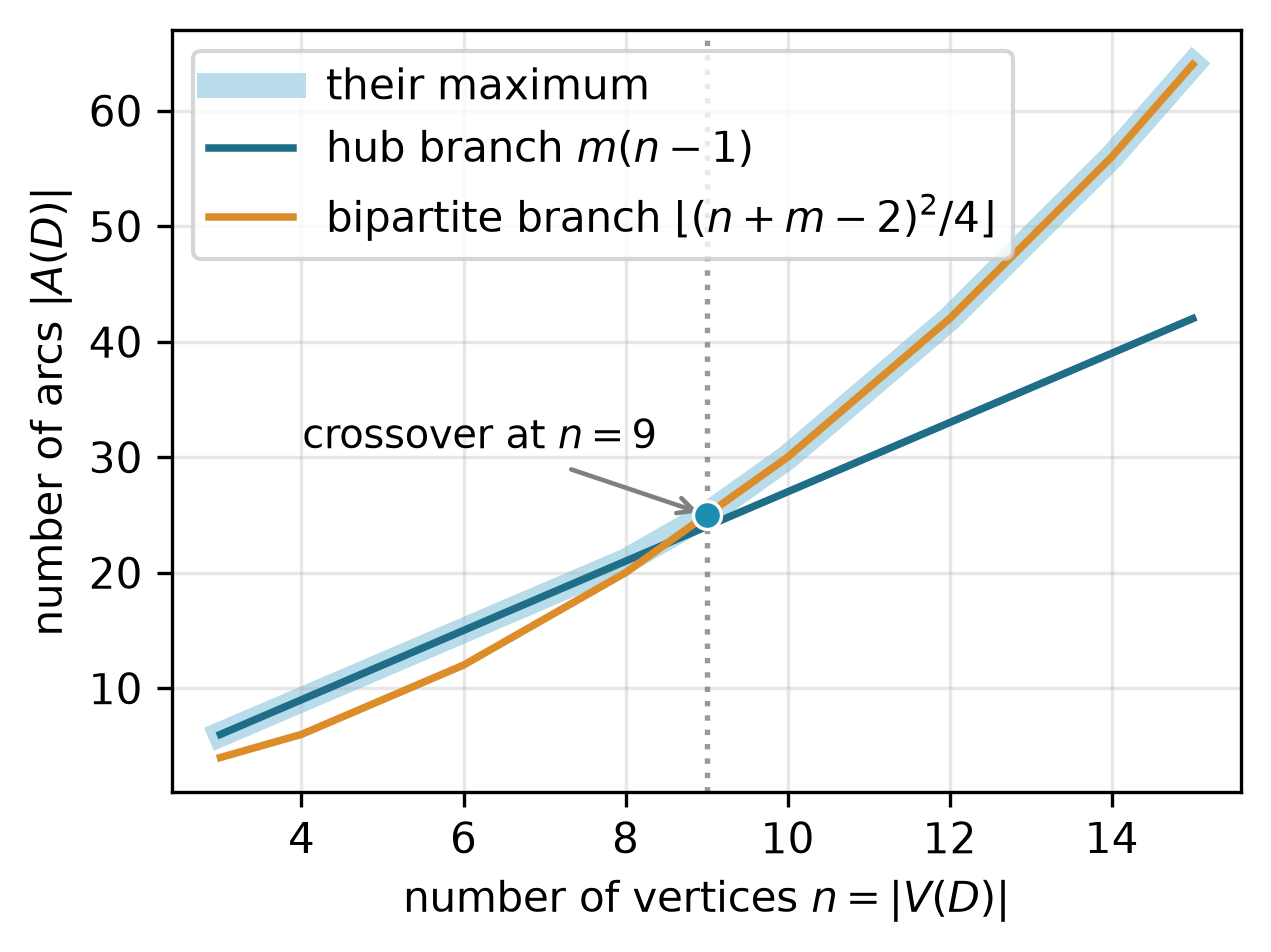
\includegraphics[width=0.78\textwidth]{figures/directed_crossover.png}
    \caption{The arc counts of the hub and of the augmented bipartite digraph at $m = 3$, and their maximum. These are lower bounds only.}
    \label{fig:crossover}
\end{figure}

\begin{figure}[t]
\centering
\begin{tikzpicture}[>=Stealth, scale=1.0,
    wallarc/.style={gdirfaint},
    cyc/.style={-{Stealth[length=2.4mm]}, line width=1.3pt, vertexorange!85!black}]

  % The m = 3, n = 10 instance: |A| = 4, |B| = 6. B is drawn as the ring its
  % m-2 = 1 cyclic in-arc per vertex actually forms, rather than as a second
  % column, where six arcs along one side merge into a single visible stroke.
  \foreach \i/\y in {1/1.65, 2/0.55, 3/-0.55, 4/-1.65} {
    \node[smallvertex] (a\i) at (0,\y) {$a_{\i}$};
  }
  \foreach \j/\ang in {1/90, 2/30, 3/-30, 4/-90, 5/-150, 6/150} {
    \node[smallvertex] (b\j) at ($(5.6,0)+(\ang:1.85)$) {$b_{\j}$};
  }
  \begin{scope}[on background layer]
    \node[draw=KULblauw1!25, fill=KULblauw1!6, rounded corners=10pt,
          fit={(a1) (a4)}, inner sep=9pt] {};
    \node[draw=vertexorange!35, fill=vertexorange!5, circle,
          fit={(b1) (b2) (b3) (b4) (b5) (b6)}, inner sep=1pt] {};
  \end{scope}
  \node[font=\scriptsize, KULblauw1] at (0,2.55) {part $A$};
  \node[font=\scriptsize, vertexorange!75!black] at (5.6,2.55) {part $B$};

  % every arc from A to B: 4 x 6 = 24
  \foreach \i in {1,...,4}{\foreach \j in {1,...,6}{\draw[wallarc] (a\i) -- (b\j);}}

  % inside B, each b_j takes its m-2 = 1 cyclic predecessor: 6 more arcs
  \foreach \j/\k in {1/2, 2/3, 3/4, 4/5, 5/6, 6/1} {
    \draw[cyc] (b\j) -- (b\k);
  }

  \node[font=\scriptsize] at (0,-2.55) {$24$ arcs $A \to B$};
  \node[font=\scriptsize, align=center, vertexorange!75!black] at (5.6,-2.55)
    {$6$ cyclic in-arcs inside $B$};
\end{tikzpicture}
\caption{The augmented bipartite digraph of \Cref{const:augmented-bipartite} at $m = 3$, $n = 10$. All arcs between the parts go from $A$ to $B$. Inside $B$, each vertex gets one arc from the previous vertex on a cycle. A pair $a_i, b_j$ has the direct arc and one detour, so $\lec^{\max} = 2$. The digraph has $24 + 6 = 30$ arcs, against $27$ for the hub.}
\label{fig:augmented-wall}
\end{figure}


\section{The reachability skeleton}\label{sec:reach-skeleton}

The next lemma is used for both exact directed results.
The proofs of \Cref{thm:dir-vertex-m2-exact,thm:dir-multi-full} in \Cref{ch:basecases} use it.

\begin{definition}[Reachability skeleton]\label{def:reach-skeleton}
Let $D$ be a directed multigraph. A \emph{reachability skeleton} of $D$ is a subdigraph $R$ on the same vertices, with at most one copy of each arc, such that for all $u\ne v$: $u$ can reach $v$ in $R$ exactly when $u$ can reach $v$ in $D$.
\end{definition}

A skeleton keeps the information about who can reach whom. It does not keep the number of disjoint paths.

\begin{lemma}[A sparse reachability skeleton always exists]\label{lem:reach-skeleton}
Every loopless directed multigraph $D$ on $n \ge 2$ vertices has a reachability skeleton $R$ with $|A(R)| \le M(n)$.
\end{lemma}

\begin{proof}
We build $R$ in three steps: first inside each strongly connected component, then between components, and then we count.
A \emph{strongly connected component} is a maximal set of vertices in which any two can reach each other.
Every digraph splits into such components.
\Cref{fig:skeleton-example} shows an example.

\emph{Step 1: inside each component.}
Take a component with $n_i$ vertices and choose a vertex $r$ in it.
Since $r$ can reach every vertex of the component, there is an \emph{out-tree}: $n_i-1$ arcs, all pointing away from $r$, along which $r$ reaches every vertex.
(Grow it one arc at a time.)
In the same way there is an \emph{in-tree} of $n_i-1$ arcs, along which every vertex reaches $r$.
Any two vertices $u,v$ of the component are then joined by a walk $u\to r\to v$ in these two trees, which contains a path.
So at most $2(n_i - 1)$ arcs keep all reachability inside the component.

\emph{Step 2: between components.}
Replace each component by one point.
Put an arc from one point to another if $D$ has an arc from the first component to the second.
This gives a digraph $Q_0$ on $q$ points, one per component.
$Q_0$ has no directed cycle, since a cycle would merge components.
Now delete arcs from $Q_0$ one at a time, as long as this does not change who can reach whom.
Call the result $Q$.

The graph $Q$, with directions ignored, has no triangle.
Indeed, suppose three points $x, y, z$ of $Q$ are joined in pairs.
Since $Q$ has no directed cycle, the three arcs must look like $x \to y$, $y \to z$ and $x \to z$, after renaming.
But then $x \to z$ could be deleted, since $x$ still reaches $z$ through $y$.
This contradicts the choice of $Q$.
By Mantel's theorem \cite{Mantel07,Turan41}, a triangle-free graph on $q$ vertices has at most $\floor{q^2/4}$ edges. So
\[
    |A(Q)| \;\le\; \floorfrac{q^2}{4}.
\]

\emph{Step 3: counting.}
Let $R$ consist of the two trees of Step 1 in every component, and, for each arc of $Q$, one arc of $D$ between the corresponding components.
By Step 1, reachability inside each component is kept.
By Step 2, reachability between components is kept: a route can follow the arcs of $Q$ and move inside each component along the trees.
Since $R \subseteq D$, $R$ creates no new reachability. So $R$ is a reachability skeleton.
If the components have sizes $n_1, \dots, n_q$, then
\[
    |A(R)| \;\le\; \sum_{i=1}^{q} 2(n_i - 1) \;+\; |A(Q)| \;\le\; 2(n-q) \;+\; \floorfrac{q^2}{4} \;=:\; f(q).
\]

It remains to bound $f(q)$ for $1 \le q \le n$.
Since $\floor{(q+1)^2/4} - \floor{q^2/4} = \floor{(q+1)/2}$ (check even and odd $q$),
\[
    f(q+1) - f(q) \;=\; -2 \;+\; \floorfrac{q+1}{2}.
\]
These differences never decrease, so $f$ is convex.
A convex function on $\{1,\dots,n\}$ is largest at $q=1$ or at $q=n$.
Since $f(1) = 2(n-1)$ and $f(n) = \floor{n^2/4}$, we get $f(q) \le M(n)$.
\end{proof}

\begin{figure}[htbp]
\centering
\resizebox{\textwidth}{!}{%
\begin{tikzpicture}
% ---- left panel: D, three bidirected SCCs A={a1,a2}, B={b1,b2}, C={c1,c2},
% joined a2->b1, b2->c1, and the redundant direct arc a1->c2 bent well below
% everything so it never crosses the other arcs.
\begin{scope}
  \node[apxlab] (a1) at (0,1) {$a_1$};
  \node[apxlab] (a2) at (0,-1) {$a_2$};
  \node[apxlab] (b1) at (2.6,1) {$b_1$};
  \node[apxlab] (b2) at (2.6,-1) {$b_2$};
  \node[apxlab] (c1) at (5.2,1) {$c_1$};
  \node[apxlab] (c2) at (5.2,-1) {$c_2$};
  \draw[aparc] (a1) to[bend left=14]  (a2);
  \draw[aparc] (a2) to[bend left=14]  (a1);
  \draw[aparc] (b1) to[bend left=14]  (b2);
  \draw[aparc] (b2) to[bend left=14]  (b1);
  \draw[aparc] (c1) to[bend left=14]  (c2);
  \draw[aparc] (c2) to[bend left=14]  (c1);
  \draw[aparc] (a2) to[bend left=8] (b1);
  \draw[aparc] (b2) to[bend left=8] (c1);
  \draw[apfaint] (a1) to[bend right=55] (c2);
  \node[apname, text=black!55] at (2.6,-2.35) {redundant: $a_1$ already reaches $c_2$ via $a_2,b_1,b_2,c_1$};
  \node[font=\small] at (2.6,2.0) {$D$};
\end{scope}
% ---- arrow between panels ----
\draw[-{Stealth[length=6pt]}, line width=1.3pt, KULblauw3b] (6.6,0) -- (7.9,0);
\node[font=\scriptsize, align=center, text=KULblauw3b] at (7.25,0.5) {drop the\\redundant arc};
% ---- right panel: R, same six vertices, same six internal arcs, only the
% two witness arcs a2->b1 and b2->c1 survive between components.
\begin{scope}[xshift=9.6cm]
  \node[apxlab] (ra1) at (0,1) {$a_1$};
  \node[apxlab] (ra2) at (0,-1) {$a_2$};
  \node[apxlab] (rb1) at (2.6,1) {$b_1$};
  \node[apxlab] (rb2) at (2.6,-1) {$b_2$};
  \node[apxlab] (rc1) at (5.2,1) {$c_1$};
  \node[apxlab] (rc2) at (5.2,-1) {$c_2$};
  \draw[aparc] (ra1) to[bend left=14]  (ra2);
  \draw[aparc] (ra2) to[bend left=14]  (ra1);
  \draw[aparc] (rb1) to[bend left=14]  (rb2);
  \draw[aparc] (rb2) to[bend left=14]  (rb1);
  \draw[aparc] (rc1) to[bend left=14]  (rc2);
  \draw[aparc] (rc2) to[bend left=14]  (rc1);
  \draw[aparc] (ra2) to[bend left=8] (rb1);
  \draw[aparc] (rb2) to[bend left=8] (rc1);
  \node[font=\small] at (2.6,2.0) {$R$};
\end{scope}
\end{tikzpicture}}
\caption[A reachability skeleton]{The construction of \Cref{lem:reach-skeleton}. Each bidirected pair $A,B,C$ is a strongly connected component. Contracting the pairs gives $A\to B\to C$ and the redundant arc $A\to C$. Delete that arc to obtain the triangle-free digraph $Q$. The skeleton $R$ keeps the internal arcs of each pair and the two remaining connections between pairs. Although $a_1\to c_2$ is removed, $a_1$ still reaches $c_2$ through $B$.}
\label{fig:skeleton-example}
\end{figure}

\begin{lemma}[The augmented bipartite digraph is feasible]\label{lem:augmented-feasible}
For $m \ge 2$ and $n \ge m$, the digraph of \Cref{const:augmented-bipartite} satisfies $\lec^{\max} = m-1$ and has $\floor{(n+m-2)^2/4}$ arcs. Hence $\ell_m^{\mathrm{dir}}(n) \ge \floor{(n+m-2)^2/4}$.
\end{lemma}

\begin{proof}
Each vertex of $B$ receives one arc from every vertex of $A$ and $m-2$ arcs from inside $B$.
So the number of arcs is $|B|\,(|A| + m - 2)$.
Here $|A| + m - 2 = \floor{(n+m-2)/2}$ and $|B| = \ceil{(n+m-2)/2}$, and $\floor{N/2}\ceil{N/2}=\floor{N^2/4}$ for every integer $N$.

Now take $a \in A$ and $b \in B$.
The direct arc and the $m-2$ routes $a \to b' \to b$ through the in-neighbours $b'$ of $b$ in $B$ are arc-disjoint.
No route from $a$ can enter $A$ again.
So every $a$--$b$ route ends with $a\to b$ or with one of the $m-2$ arcs into $b$ from $B$.
Removing these $m-1$ arcs separates $a$ from $b$, so $\lec(a,b) = m-1$.
For $b_i, b_j \in B$, a route from $b_i$ stays in $B$, so it ends with one of the $m-2$ arcs into $b_j$ from $B$, and $\lec(b_i,b_j)\le m-2$.
There are no routes from $B$ to $A$ or inside $A$.
So $\lec^{\max} = m - 1$.
\end{proof}

\section{Simple digraphs beyond the first threshold}

\subsection{The two-step budget}\label{sec:two-step-budget}

\begin{definition}[Two-step budget]\label{def:two-step-budget}
Let $D$ be a simple digraph and $C \ge 1$. For $u\ne v$, let $p_2(u,v)$ be the number of vertices $x \notin \{u,v\}$ with arcs $u\to x$ and $x\to v$. Such an $x$ is the \emph{midpoint} of the route $u \to x \to v$. We call $D$ \emph{$C$-budgeted} if every ordered pair $(u,v)$ of distinct vertices satisfies
\[
    \mathbf{1}_{(u,v) \in A(D)} + p_2(u,v) \;\le\; C .
\]
\end{definition}

\begin{lemma}[Feasible digraphs are budgeted]\label{lem:feasible-budgeted}
Let $D$ be a simple digraph and $m \ge 2$. If $\lec^{\max}_D \le m-1$, or if $\kap^{\max}_D \le m-1$, then $D$ is $(m-1)$-budgeted.
\end{lemma}

\begin{proof}
Fix an ordered pair $(u,v)$.
Take the arc $u\to v$, if it exists, and the route $u\to x\to v$ for each of the $p_2(u,v)$ midpoints $x$.
Two routes with different midpoints use different arcs, and none of them uses the arc $u\to v$.
So these routes are arc-disjoint.
Each two-step route has one inner vertex, its midpoint, and the arc has none.
So the routes are also internally vertex-disjoint.
So their number is at most $\lec_D(u,v)$ and at most $\kap_D(u,v)$, and either condition gives at most $m-1$.
\end{proof}

The next lemma turns the budget into a statement about degrees.
A vertex with large in-degree and large out-degree is the midpoint of many two-step routes, and the budget limits these.

\begin{lemma}[The budget, read on degrees]\label{lem:budget-degree-sum}
Every $C$-budgeted simple digraph $D$ on $n$ vertices satisfies
\[
    \sum_{x \in V} d^+(x)\,d^-(x) \;\le\; C\,n(n-1) .
\]
\end{lemma}

\begin{proof}
Count the walks $u \to x \to v$ of length two.
Choosing the middle vertex $x$, an in-neighbour $u$ and an out-neighbour $v$ gives $\sum_x d^-(x)\,d^+(x)$ walks.
The walks with $u \ne v$ number $\sum_{u\ne v} p_2(u,v)$.
A walk with $u = v$ is fixed by its first arc $u \to x$, so there are at most $|A(D)|$ of them.
Summing the budget over all ordered pairs gives $|A(D)| + \sum_{u\ne v} p_2(u,v) \le C\,n(n-1)$. So
\[
    \sum_x d^+(x)\,d^-(x) \;\le\; \sum_{u\ne v} p_2(u,v) + |A(D)| \;\le\; C\,n(n-1). \qedhere
\]
\end{proof}

\begin{lemma}[Deleting the smaller half of every vertex]\label{lem:smaller-half-deletion}
Every simple digraph $D$ on $n$ vertices can be made \emph{one-way bipartite}, so that all remaining arcs go from one part to the other, by deleting at most $\sum_{x} \min(d^+(x), d^-(x))$ arcs. So
\[
    |A(D)| \;\le\; \floorfrac{n^2}{4} \;+\; \sum_{x \in V} \min\bigl(d^+(x), d^-(x)\bigr) .
\]
\end{lemma}

\begin{proof}
Call $x$ \emph{source-like} if $d^+(x) \ge d^-(x)$, and \emph{sink-like} otherwise. Let $S$ and $T$ be these two sets.
Delete every arc into a source-like vertex and every arc out of a sink-like vertex.
At each vertex $x$ this deletes $\min(d^+(x), d^-(x))$ arcs, so in total at most the sum above.
An arc $a\to b$ survives only if $a \in S$ and $b \in T$.
So the remaining arcs all go from $S$ to $T$, and there are at most $|S|\,|T|\le\floor{n^2/4}$ of them.
\end{proof}

\begin{lemma}[The counting core]\label{lem:two-step-budget}
Every $C$-budgeted simple digraph $D$ on $n \ge 2$ vertices satisfies
\[
    |A(D)| \;\le\; \floorfrac{n^2}{4} \;+\; 4C(n-1).
\]
\end{lemma}

\begin{proof}
We use induction on $n$.
For $n = 2$ a simple digraph has at most $2$ arcs, and the right side is $1 + 4C \ge 5$.
Let $n \ge 3$.

First suppose some vertex $v$ has total degree $d(v) < n/2$, so $d(v) \le \floor{n/2}$.
Deleting $v$ only removes routes, so $D-v$ is still $C$-budgeted.
By induction, and since $\floor{(n-1)^2/4}+\floor{n/2}=\floor{n^2/4}$ (check even and odd $n$),
\[
\begin{aligned}
    |A(D)|
    &\le \floorfrac{(n-1)^2}{4}+4C(n-2)+\floorfrac n2 \\
    &= \floorfrac{n^2}{4}+4C(n-2)
    \le \floorfrac{n^2}{4}+4C(n-1).
\end{aligned}
\]

Otherwise $d(x) \ge n/2$ for every vertex.
For $a,b\ge0$ with $a+b>0$ we have $\min(a,b)\le2ab/(a+b)$, since $\max(a,b)\ge(a+b)/2$.
With $a=d^+(x)$, $b=d^-(x)$ and \Cref{lem:budget-degree-sum} this gives
\[
    \sum_x\min\bigl(d^+(x),d^-(x)\bigr)
    \;\le\; \frac{2}{\min_x d(x)}\sum_x d^+(x)d^-(x)
    \;\le\; \frac4n\,C\,n(n-1)
    \;=\; 4C(n-1),
\]
and \Cref{lem:smaller-half-deletion} gives the claim.
\end{proof}

We can now prove \Cref{thm:dir-arc-linear-error}.

\begin{proof}[Proof of \Cref{thm:dir-arc-linear-error}]
By \Cref{lem:feasible-budgeted} a simple digraph with $\lec^{\max}_D \le m-1$ or with $\kap^{\max}_D \le m-1$ is $(m-1)$-budgeted, so \Cref{lem:two-step-budget} at $C = m-1$ gives the stated bound.

For the lower bound, \Cref{const:augmented-bipartite} has $\lec^{\max} \le m-1$, so also $\kap^{\max} \le m-1$. For $n\ge m$ this gives
\[
    k_m^{\mathrm{dir}}(n) \;\ge\; \ell_m^{\mathrm{dir}}(n) \;\ge\; \floorfrac{(n+m-2)^2}{4}
    \;=\; \frac{n^2}{4} + \frac{(m-2)n}{2} + O_m(1).
\]
So for $m\ge3$ the second term is linear in $n$ on both sides.
\end{proof}

The linear coefficient is not known.
The construction gives $(m-2)n/2$, and \Cref{thm:dir-arc-linear-error} allows $4(m-1)n$.
For large $n$ a theorem of Huang and Lyu \cite[Theorem~2]{HuangLyu26}, with $t=m-1$, lowers this to $(m-1)n$.
It applies because a feasible digraph has at most $m-1$ paths of length two between any two vertices (\Cref{lem:feasible-budgeted}).
Our bound is weaker, but it holds for every $n$.




The next proposition is about the shape of a feasible digraph.
After deleting $O(\sqrt m\,n^{3/2})$ arcs, all remaining arcs go from one part to the other.
The parts need not be balanced.
For fixed $m$ this error is larger than the linear error of \Cref{thm:dir-arc-linear-error}.

\begin{proposition}[Almost all arcs go one way]\label{prop:dir-arc-stability}
Let $D$ be a simple digraph on $n \ge 2$ vertices with $\lec^{\max}_D \le m-1$. Then deleting at most $\sqrt{m}\, n^{3/2}$ arcs leaves $D$ a subgraph of a one-directional bipartite digraph, and
\[
    |A(D)| \;\le\; \floorfrac{n^2}{4} \;+\; \sqrt{m}\, n^{3/2}.
\]
\end{proposition}

\begin{proof}
By \Cref{lem:feasible-budgeted}, $D$ is $(m-1)$-budgeted.
We use $\min(a,b) \le \sqrt{ab}$, the Cauchy--Schwarz inequality $\sum_x \sqrt{a_x} \le \sqrt{n \sum_x a_x}$, and \Cref{lem:budget-degree-sum}:
\[
\begin{aligned}
    \sum_{x \in V} \min\bigl(d^+(x), d^-(x)\bigr)
    &\;\le\; \sum_{x \in V} \sqrt{d^+(x)\, d^-(x)}
    \;\le\; \sqrt{\,n \sum_{x \in V} d^+(x)\, d^-(x)\,} \\[2pt]
    &\;\le\; \sqrt{\,n \cdot (m-1)\,n(n-1)\,}
    \;=\; n\sqrt{(m-1)(n-1)}
    \;\le\; \sqrt{m}\, n^{3/2}.
\end{aligned}
\]
\Cref{lem:smaller-half-deletion} now gives both statements.
\end{proof}



So for $m\ge3$ both directed problems have leading term $n^2/4$ and a linear second term. The linear coefficient and the exact values are open. It is also open whether the two values are equal.

\section{The extremal directed multigraphs}\label{sec:dir-multi}

At $m=2$ a feasible directed multigraph has no parallel arcs. So \Cref{thm:dir-multi-full} at $m=2$ is \Cref{thm:dir-arc-m2-exact}.


\label{sec:quadratic-uniqueness}

\Cref{thm:dir-multi-full} gives the value, but not the extremal multigraphs.
This subsection describes them for large $n$.
The idea is to look at the proof of \Cref{lem:reach-skeleton} in the case of equality.
Equality fixes the number of strongly connected components, then the shape of the skeleton, and then the multigraph.


\begin{lemma}[What equality forces]\label{lem:equality-forces}
Let $m\ge2$ and $n \ge 8$, so that $\floor{n^2/4} > 2(n-1)$ and $M(n) = \floor{n^2/4}$, and let $D$ be a directed multigraph on $n$ vertices with $\lec^{\max}_D \le m-1$ and $|A(D)| = (m-1)\floor{n^2/4}$. Then
\begin{enumerate}[label=(\arabic*)]
    \item $D$ is \emph{acyclic}: it has no directed cycle, and
    \item $D$ has a reachability skeleton $R$ from which no arc can be removed without changing who reaches whom, and which, with directions ignored, is the complete bipartite graph $K_{\ceil{n/2},\floor{n/2}}$.
\end{enumerate}
\end{lemma}

\begin{proof}
The proof of \Cref{thm:dir-multi-full} removes skeletons $R_1, \dots, R_{m-1}$, and then no arc is left. So $|A(D)| = \sum_i |A(R_i)|$.
Each $|A(R_i)| \le M(n)$, so equality forces $|A(R_i)| = M(n)$ for every $i$. Let $R := R_1$.

In the proof of \Cref{lem:reach-skeleton}, $|A(R)| \le f(q) = 2(n-q) + \floor{q^2/4}$, where $q$ is the number of strongly connected components. So $f(q) \ge \floor{n^2/4} = f(n)$.
Since $n\ge8$, $f(1)=2(n-1) < \floor{n^2/4} = f(n)$.
The function $f$ is convex, so between $1$ and $n$ it stays below the straight line from $f(1)$ to $f(n)$.
That line lies below $f(n)$ except at $q=n$, so $f(q) < f(n)$ for $q<n$.
So $q = n$: every strongly connected component is a single vertex. This is (1).

With $q = n$ the trees of Step 1 are empty, so $R$ consists of the arcs chosen for $Q$, and $|A(Q)| = \floor{n^2/4}$.
The graph $Q$ is triangle-free, and a triangle-free graph on $n$ vertices with $\floor{n^2/4}$ edges is $K_{\ceil{n/2},\floor{n/2}}$ (the equality case of Mantel's theorem \cite{Mantel07}).
This is (2). The skeleton $R$ is acyclic because $D$ is, and no arc of $R$ can be removed without changing reachability, because the same holds for $Q$.
\end{proof}

The next lemma uses that no arc of $R$ can be removed.

\begin{lemma}[A minimal bipartite skeleton has no long path]\label{lem:skeleton-shallow}
Let $R$ be as in \Cref{lem:equality-forces}, with parts $A$ and $B$. Then $R$ contains no directed path with three arcs.
\end{lemma}

\begin{proof}
Suppose $u \to v \to w \to x$ is such a path.
The path alternates between the parts, so $u$ and $x$ lie in different parts.
The underlying graph of $R$ is complete bipartite, so $R$ has an arc between $u$ and $x$.
It cannot be $x \to u$, since that would close a directed cycle, and $D$ is acyclic.
So $u \to x$ is in $R$.
But $u$ also reaches $x$ along the path, so $u\to x$ could be removed without changing reachability. This is a contradiction.
\end{proof}

\begin{theorem}[Extremal classification on the quadratic branch]\label{thm:dir-multi-uniqueness}
Let $m \ge 2$ and $n \ge \max(8,\, 2m)$, so that $M(n) = \floor{n^2/4}$ and $n$ is on the quadratic branch. If $D$ is a directed multigraph on $n$ vertices with $\lec^{\max}_D \le m-1$ and $|A(D)| = L_m^{\mathrm{dir}}(n) = (m-1)\floor{n^2/4}$, then
\[
    D \;\in\; \left\{(m-1) \cdot B_{\ceil{n/2},\,\floor{n/2}},\ (m-1) \cdot B_{\floor{n/2},\,\ceil{n/2}}\right\} ,
\]
where $B_{a,b}$ has all arcs from its part of size $a$ to its part of size $b$, each once, and $(m-1)\cdot B_{a,b}$ takes every arc $m-1$ times as in \Cref{lem:thickening}. These two digraphs are the same up to renaming the vertices when $n$ is even, and reverses of each other when $n$ is odd.
\end{theorem}

\begin{proof}
Take $R$, $A$ and $B$ from \Cref{lem:equality-forces}, and write $\alpha = |A| \ge \beta = |B| = \floor{n/2}$.

\emph{Step 1: $R$ has no directed path with two arcs.}
Suppose $a \to b \to a'$ with $a, a' \in A$ and $b \in B$.
If $a$ had an incoming arc $b_0 \to a$, then $b_0 \to a \to b \to a'$ would be a path with three arcs, which \Cref{lem:skeleton-shallow} forbids.
So $a$ has no incoming arc. Since the underlying graph is complete bipartite, $a \to b''$ for every $b'' \in B$.
In the same way $a'$ has no outgoing arc, so $b'' \to a'$ for every $b'' \in B$.
The $\beta$ routes $a \to b'' \to a'$ use different arcs.
So $\lec_D(a,a') \ge \beta = \floor{n/2} \ge m$, which breaks the condition.
A path $b \to a \to b'$ is excluded in the same way, since $\alpha \ge \beta \ge m$.
This is the only step that uses $n \ge 2m$.

\emph{Step 2: all arcs of $R$ go the same way.}
By Step 1, no vertex of $R$ has both an incoming and an outgoing arc.
Take $a \in A$. It is joined to every vertex of $B$.
If all arcs at $a$ go out, then every $b\in B$ has an incoming arc, so it has no outgoing arc. So all arcs go from $A$ to $B$.
If all arcs at $a$ come in, all arcs go from $B$ to $A$ in the same way.
From now on, call the part that the arcs leave $A$, and the other part $B$.

\emph{Step 3: $D$ has no arc outside $R$.}
In $R$, the only pairs $(u,x)$ with $u$ reaching $x$ are the pairs in $A \times B$, and each such pair is an arc of $R$.
If $D$ has an arc $u\to x$, then $u$ reaches $x$ in $D$, so also in $R$. So $u\to x$ is an arc of $R$.

\emph{Step 4: every multiplicity is $m-1$.}
Parallel arcs are disjoint routes, so every multiplicity is at most $m-1$.
There are $|A||B|\le\floor{n^2/4}$ pairs, and $|A(D)| = (m-1)\floor{n^2/4}$.
So every pair has multiplicity $m-1$, and $|A||B|=\floor{n^2/4}$, so the parts have sizes $\ceil{n/2}$ and $\floor{n/2}$.
\end{proof}

The hypothesis $n\ge2m$ is used only in Step 1. Every vertex of an extremiser has degree at least $(m-1)\floor{n/2}$, because deleting it leaves at most $(m-1)M(n-1)$ arcs. For even $n$, every vertex has degree exactly $(m-1)n/2$.


\apppart{Part III. Hypergraphs}{Menger for hypergraphs, simple hypergraphs that attain the edge bound, the vertex problem at $m = 3$, multigraphs with vertex separation, and directed hypergraphs.}

\section{The hypergraph bounds}

There are several notions of connectivity in hypergraphs, for example in Chekuri and Xu \cite{ChekuriXu17} and Dewar, Pike and Proos \cite{DewarPikeProos18}.
This thesis uses Berge paths throughout.
We first need Menger's theorem for Berge paths. It also shows that the gate network of \Cref{ch:certify} computes the right value.

\begin{theorem}[Menger for multihypergraphs]\label{thm:menger-hyper}
Let $u,v$ be distinct vertices of a multihypergraph $\HH$, and count parallel copies of a hyperedge separately. The largest number of $u$--$v$ Berge paths that share no hyperedge copy equals the smallest number of hyperedge copies whose removal separates $u$ from $v$.
\end{theorem}

\begin{proof}
We turn $\HH$ into a directed multigraph $N$, the gate network of \Cref{fig:hyper-gadget}, and use Menger's theorem for directed multigraphs (\Cref{thm:menger}).
Let $c$ be the total number of hyperedge copies.
Every hyperedge $e$ with $\mu(e)$ copies gets two new nodes $e^-$ and $e^+$ and $\mu(e)$ parallel arcs $e^- \to e^+$, its \emph{gate}.
Every vertex $x \in e$ gets $c+1$ parallel arcs $x \to e^-$ and $c+1$ parallel arcs $e^+ \to x$.

\emph{Paths.} A Berge path $u, e_1, v_1, \dots, e_k, v$ becomes the directed path $u \to e_1^- \to e_1^+ \to v_1 \to \cdots \to v$, and back.
In a family of Berge paths that share no copy, at most $\mu(e)$ paths use $e$, so each can take its own gate arc.
There are enough copies of the other arcs.
So arc-disjoint directed paths in $N$ and Berge paths that share no copy come in families of the same sizes.

\emph{Cuts.} Removing all $c$ gate arcs separates $u$ from $v$.
So a smallest separating set of arcs in $N$ has at most $c$ arcs, and never removes all $c+1$ copies of a non-gate arc.
Removing only some copies changes nothing, so a smallest separating set consists of gate arcs only, and it takes all gate arcs of a hyperedge or none.
Such a set separates $u$ from $v$ in $N$ exactly when the same hyperedge copies separate $u$ from $v$ in $\HH$.

So both sides of Menger's theorem have the same value in $N$ and in $\HH$.
\end{proof}

The same proof works for directed hyperedges and directed Berge paths, with arcs $x \to e^-$ only for the tails $x$ of $e$, and arcs $e^+ \to x$ only for its heads.

The next theorem shows that for $r \ge 3$ and $m-1\le\binom{n-2}{r-2}$, simple hypergraphs attain the same bound.
For graphs ($r=2$) this is different: there, simplicity lowers the bound from $(m-1)(n-1)$ to $\floor{m(n-1)/2}$.



\begin{theorem}[Simplicity is free for $r \ge 3$]\label{thm:simple-hyper-edge}
Let $r \ge 3$, $n \ge r$, and $2 \le m$ with $m-1 \le \binom{n-2}{r-2}$. Then the maximum number of hyperedges in a \emph{simple} $r$-uniform hypergraph on $n$ vertices with $\lec^{\max}\le m-1$ is exactly $\floorfrac{(m-1)(n-1)}{r-1}$.
\end{theorem}

\begin{proof}
The upper bound is \Cref{prop:hyper-edge}.
For the lower bound, take a hub $h$ and let $V' = V \setminus \{h\}$.
By \Cref{lem:sparse-hypergraph} with uniformity $r-1$ and degree bound $d = m-1$ on the $n-1$ vertices of $V'$, there is a simple $(r-1)$-uniform hypergraph $\mathcal{G}^*$ on $V'$ with maximum degree at most $m-1$ and $\floorfrac{(m-1)(n-1)}{r-1}$ hyperedges.
Add $h$ to each of its hyperedges. The new hyperedges are different $r$-sets, so the result $\HH$ is simple.
Every vertex $w \ne h$ lies in at most $m-1$ hyperedges, and every route from or to $w$ uses one of them.
Every pair contains such a vertex, so $\lec^{\max}_\HH \le m-1$.
\end{proof}

\begin{remark}[The condition is needed]\label{rem:simple-hyper-necessary}
Without the condition $m-1\le\binom{n-2}{r-2}$, simple hypergraphs may not reach the bound.
The smallest example is $n = r = m = 3$.
There is only one $3$-set, so a simple hypergraph has at most one hyperedge, while the bound is $\floor{2 \cdot 2 / 2} = 2$.
Two copies of the one hyperedge do reach the bound.
\Cref{thm:hyper-vertex-m3} needs the same condition with $m - 1 = 2$, which is the range $2 < r < n$.
\end{remark}

\begin{construction}[Twelve hyperedge copies on six vertices]\label{const:multihyper-six}
Take a hub $h$ and five other vertices $a,b,c,d,e$. Include all ten triples
consisting of $h$ and two of the other vertices. Add a second copy of
$\{h,d,e\}$ and one copy of $\{a,b,c\}$. The resulting $3$-uniform
multihypergraph has $12$ hyperedge copies and $\lec^{\max}\le5$.
Consequently, the multihypergraph edge value at $(n,m,r)=(6,6,3)$ is exactly
$12$, even though $(r-1)$ does not divide $(n-1)$.
\end{construction}

\begin{proof}
Initially each non-hub vertex lies in four of the ten triples. The repeated
triple raises the degrees of $d$ and $e$ to five, while the final triple does
the same for $a$, $b$ and $c$. Every pair of distinct vertices therefore
includes a non-hub vertex whose five incident hyperedge copies form a cut
separating it from the other endpoint. Thus no pair has more than five
hyperedge-disjoint routes. The construction has $10+1+1=12$ copies, matching
the upper bound $\floor{5(6-1)/(3-1)}=12$ from \Cref{prop:hyper-edge}.
\end{proof}

Since $\kap\le\lec$, the same multihypergraph also gives $12$ for the vertex problem. We do not know whether $12$ is optimal there.



\section{The hypergraph vertex problem}\label{sec:hyper-vertex-proof}

The vertex problem for hypergraphs becomes a problem about graphs (\Cref{fig:incidence}).
Recall the \emph{incidence graph} $I(\HH)$: one node per vertex, one node per hyperedge, and an edge when the vertex lies in the hyperedge.
A Berge path is the same as a path in $I(\HH)$ between two vertex nodes.
Its inner nodes are the hyperedges it uses and the vertices where it changes hyperedge.
So two Berge routes share no hyperedge and no inner vertex exactly when the two paths in $I(\HH)$ are internally disjoint.
So
\[
    \kap_\HH(u, v) \;=\; \kap_{I(\HH)}(u, v).
\]
The vertex problem asks for the largest number of hyperedge nodes, each of degree $r$, such that no two of the $n$ vertex nodes are joined by $m$ internally disjoint paths.

\begin{figure}[htbp]
\centering
\begin{subfigure}[b]{0.99\textwidth}
\centering
\begin{tikzpicture}[scale=1.0]
% ----- left: hypergraph H, 3-uniform, vertices 1..6, hyperedges e1,e2,e3 ---
\begin{scope}
  % the Berge-path stations 1,3,5 sit on a baseline, the extra members 2,4,6
  % above, so each hyperedge is a clean metro line arcing over the path.
  % labels sit INSIDE the vertices, the convention the body uses throughout
  \node[apxlab] (1) at (0.0, 0.0) {$1$};
  \node[apxlab] (2) at (1.1, 1.3) {$2$};
  \node[apxlab] (3) at (2.2, 0.0) {$3$};
  \node[apxlab] (4) at (3.3, 1.3) {$4$};
  \node[apxlab] (5) at (4.4, 0.0) {$5$};
  \node[apxlab] (6) at (5.5, 1.3) {$6$};
  % hyperedges as metro lines, each its own colour: e1 red, e2 blue, e3 grey.
  \begin{scope}[on background layer]
    \draw[metro, metroA]  (1)--(2)--(3);   % e1 = {1,2,3}
    \draw[metro, metroB]  (3)--(4)--(5);   % e2 = {3,4,5}
    \draw[metro, metroF] (4)--(6)--(5);  % e3 = {4,5,6}, off the path
  \end{scope}
  \node[apname, text=metroA]   at (0.55,1.05) {$e_1$};
  \node[apname, text=metroB]   at (2.75,1.05) {$e_2$};
  \node[apname, text=metroF] at (6.05,1.3) {$e_3$};
  % Berge path 1 -e1- 3 -e2- 5: orange arrows along the baseline, clear of lines
  \draw[line width=2pt, vertexorange, -{Stealth[length=2.4mm]}] (1)--(3);
  \draw[line width=2pt, vertexorange, -{Stealth[length=2.4mm]}] (3)--(5);
  \node[apname, text=vertexorange!85!black] at (2.2,-0.75) {Berge path $1\,e_1\,3\,e_2\,5$};
  \node[font=\small] at (2.75,-1.5) {hypergraph $\HH$};
\end{scope}
% arrow
\draw[-{Stealth[length=6pt]}, line width=1.3pt, KULblauw3b]
   (5.7,0.55) -- (6.6,0.55);
% ----- right: incidence graph I(H): vertices (circles) | hyperedges (squares)
\begin{scope}[xshift=7.0cm]
  \foreach \i/\y in {1/2.2,2/1.3,3/0.4,4/-0.5,5/-1.4,6/-2.3}{
    \node[apxlab] (n\i) at (0,\y) {$\i$};
  }
  \node[apz] (E1) at (2.4,1.3) {$e_1$};
  \node[apz] (E2) at (2.4,-0.5){$e_2$};
  \node[apz] (E3) at (2.4,-2.0){$e_3$};
  % incidences (path 1-e1-3-e2-5 traced orange to match the left; rest light)
  \draw[apgedge] (n2)--(E1);
  \draw[apgedge] (n4)--(E2);
  \draw[apgedge] (n4)--(E3);
  \draw[apgedge] (n5)--(E3);
  \draw[apgedge] (n6)--(E3);
  \draw[apgedge,vertexorange,line width=2pt] (n1)--(E1);
  \draw[apgedge,vertexorange,line width=2pt] (n3)--(E1);
  \draw[apgedge,vertexorange,line width=2pt] (n3)--(E2);
  \draw[apgedge,vertexorange,line width=2pt] (n5)--(E2);
  \node[font=\small] at (1.2,-3.0) {incidence graph $I(\HH)$};
\end{scope}
\end{tikzpicture}
\caption{A $3$-uniform hypergraph $\HH$ (left) and its bipartite incidence
graph $I(\HH)$ (right): circles for vertices, hollow squares for hyperedges,
an edge when the vertex lies in the hyperedge. The Berge path
$1\,e_1\,3\,e_2\,5$ is traced in orange in both pictures. In $\HH$ it rides the
red line $e_1$ and the blue line $e_2$, changing at the shared vertex $3$, while
the grey line $e_3$ lies off it. In $I(\HH)$ it is the ordinary path
$1\!-\!e_1\!-\!3\!-\!e_2\!-\!5$ alternating sides.}
\label{fig:incidence-berge}
\end{subfigure}

\medskip
\begin{subfigure}[b]{0.99\textwidth}
\centering
\begin{tikzpicture}[
   stn/.style={metrostop, minimum size=5.5mm},
   hub/.style={metrostop, minimum size=8mm, draw=vertexorange!90!black,
               fill=vertexorange!45, line width=1.3pt}]
% star hypertree: each hyperedge {h,u_i,w_i} is one metro line through the hub,
% leaving radially to an inner station and bending to an outer one.
\begin{scope}[on background layer]
  \foreach \ang/\col in {90/metroA, 210/metroB, 330/metroC}{
    \draw[metro, \col] (0,0) -- (\ang:1.5) -- ({\ang+22}:2.5);
  }
\end{scope}
\foreach \ang in {90,210,330}{
  \node[stn] at (\ang:1.5) {};
  \node[stn] at ({\ang+22}:2.5) {};
}
\node[hub] at (0,0) {$h$};
\end{tikzpicture}
\caption{A star hypertree: every hyperedge $\{h\}\cup G_i$ shares only the
hub $h$ (orange), and the other $r-1=2$ vertices of each block sit in a
single hyperedge. Its incidence graph is a tree, so $\kap^{\max}\le1$.}
\label{fig:star-hypertree}
\end{subfigure}
\caption[Incidence translation]{The translation the vertex problem rests on.
Internally vertex-disjoint Berge paths in $\HH$ correspond exactly to
internally disjoint paths in $I(\HH)$, so $\kap_\HH(u,v)=\kap_{I(\HH)}(u,v)$.
\textbf{(top)} A hypergraph and its incidence graph with one Berge path
drawn in both. \textbf{(bottom)} The star hypertree of
\Cref{thm:hyper-vertex-m2}, whose incidence graph is a tree.}
\label{fig:incidence}
\end{figure}

\begin{proposition}[General lower bound]\label{prop:hyper-vertex-lower}
For $r \ge 3$, $m \ge 2$ and $m - 1 \le \binom{n-2}{r-2}$,
\[
    k_m^{(r)}(n) \;\ge\; \floorfrac{(m-1)(n-1)}{r-1},
\]
attained by a simple hypergraph.
\end{proposition}

\begin{proof}
The simple hypergraph of \Cref{thm:simple-hyper-edge} has $\lec^{\max}\le m-1$.
Since $\kap \le \lec$, it is also feasible for the vertex problem.
\end{proof}

That construction needs different $(r-1)$-sets, which explains the condition $m-1\le\binom{n-2}{r-2}$.
A multihypergraph can repeat a hyperedge instead. This covers other cases.

\begin{proposition}[The multihypergraph lower bound]\label{prop:hyper-vertex-lower-multi}
For $r \ge 2$, $m \ge 2$ and $(r-1) \mid (n-1)$,
\[
    K_m^{(r)}(n) \;\ge\; \frac{(m-1)(n-1)}{r-1},
\]
attained by the star hypertree of \Cref{fig:hyper-star} with every hyperedge
taken at multiplicity $m-1$. At $m = 3$ this meets the upper bound of
\Cref{thm:hyper-vertex-m3}, so
\[
    K_3^{(r)}(n) \;=\; \floorfrac{2(n-1)}{r-1}
    \qquad\text{whenever } (r-1) \mid (n-1).
\]

\end{proposition}

\begin{proof}
Take the hub $h$ and split the other $n-1$ vertices into groups $G_1, \dots, G_q$ of size $r-1$, where $q = (n-1)/(r-1)$.
Give each hyperedge $\{h\} \cup G_i$ multiplicity $m-1$. This gives $(m-1)q$ hyperedges.

Now take two vertices $u \ne w$.
Suppose first that both lie in $\{h\}\cup G_i$.
One of them lies in $G_i$, and every route from or to it uses one of the $m-1$ copies of $\{h\}\cup G_i$.
So $\kap(u,w) \le \lec(u,w) \le m-1$.
Now suppose $u \in G_i$ and $w \in G_j$ with $i \ne j$.
Every route from $u$ to $w$ passes through $h$, so $\kap(u,w) \le 1$.
So the hypergraph is feasible.

At $m = 3$ there are $2(n-1)/(r-1)$ hyperedges, which equals the upper bound of \Cref{thm:hyper-vertex-m3}.
\end{proof}

The upper bound at $m=3$ follows from a bound on the cycles of a graph, proved next.
For a connected multigraph $G$, the \emph{cycle rank} is $\mathrm{rank}(G) = |E(G)| - |V(G)| + 1$.
A tree has cycle rank $0$, and each extra edge raises it by one.

We use the words cut vertex and $k$-connected from \Cref{sec:simple-vertex-blocks}.
A \emph{separating pair} is a pair of vertices whose removal disconnects the graph.
By Menger's theorem \cite[Ch.~3]{Diestel17}, a graph is $3$-connected exactly when every two vertices are joined by $3$ internally disjoint paths.

\begin{lemma}[Incidence rank lemma]\label{lem:incidence-rank}
Let $G$ be a connected loopless multigraph with a partition $V(G)=X \mathbin{\dot\cup} Z$ such that
(i) no two vertices of $Z$ are adjacent, (ii) no edge incident to $Z$ is parallel to another
edge, (iii) every $z \in Z$ has degree at least $2$, and (iv)
$\kap_G(x, x') \le 2$ for all distinct $x, x' \in X$. Then
$\mathrm{rank}(G) \le |X| - 1$.
\end{lemma}

Read $X$ as the vertices of a hypergraph and $Z$ as its hyperedges, so that $G$ is the incidence graph.
Then (i) says that two hyperedge nodes are never adjacent, (ii) that no hyperedge repeats a vertex, (iii) that every hyperedge has at least two vertices, and (iv) that the hypergraph is feasible at $m = 3$.
We allow edges inside $X$, because Step~2 of the proof creates them.

\begin{proof}
We use induction on $|V| + |E|$.
Step~1 handles cut vertices.
Steps~2 and~3 remove vertices of degree two.
Step~4 handles what is left: a $2$-connected graph with minimum degree at least three.

\emph{Base: $|V| \le 2$.}
A vertex in $Z$ has degree at least $2$ by (iii), and by (ii) its edges go to different vertices.
So with at most two vertices, $Z$ is empty and all vertices lie in $X$.
With one vertex, $\mathrm{rank}=0=|X|-1$.
With two vertices, the parallel edges between them are internally disjoint routes, so by (iv) there are at most two, and $\mathrm{rank} \le 1 = |X| - 1$.

\emph{Step 1: a cut vertex.}
Suppose $G$ has a cut vertex $c$.
Split the components of $G-c$ into two non-empty groups.
Let $G_1$ and $G_2$ consist of $c$ together with the first and the second group, with all their edges.
They share only the vertex $c$, so $\mathrm{rank}(G) = \mathrm{rank}(G_1) + \mathrm{rank}(G_2)$.
Each $G_i$ is connected and smaller than $G$, and (i), (ii) and (iv) still hold in it.
Condition (iii) can only fail at $c$, when $c \in Z$ has a single neighbour in $G_i$.
Then delete $c$ from $G_i$. This removes one vertex and one edge, so the rank and the set of $X$-vertices do not change.
By induction, $\mathrm{rank}(G_i) \le |X \cap V(G_i)| - 1$.
The two $X$-sets together have $|X|+1$ vertices if $c \in X$, and $|X|$ vertices if $c \in Z$.
Either way $\mathrm{rank}(G) \le (|X| + 1) - 2 = |X| - 1$.

\emph{Step 2: a $Z$-vertex of degree two.}
From now on $G$ has no cut vertex and at least three vertices, so it is $2$-connected.
Suppose some $z_0 \in Z$ has degree $2$.
By (i) its two neighbours $x, x'$ lie in $X$, and by (ii) they are different.
\emph{Suppress} $z_0$: delete it and add a new edge $xx'$.
Then $|E|$ and $|V|$ both drop by one, so the rank does not change.
The new edge lies inside $X$, so $|X|$ does not change, and (i), (ii), (iii) still hold.
A route through $z_0$ becomes a route through the new edge, so every $\kap(x_1, x_2)$ stays the same and (iv) holds.
The graph is smaller, so the induction hypothesis gives the bound.

\emph{Step 3: an $X$-vertex of degree two.}
Now every $Z$-vertex has degree at least $3$.
Suppose some $x_0 \in X$ has degree $2$, and delete it.
Since $G$ is $2$-connected, the result is connected.
We remove two edges and one vertex, so the rank drops by one, and $|X|$ drops by one.
A neighbour in $Z$ keeps degree at least $2$, so (iii) holds.
Deleting a vertex cannot raise a connectivity, so (iv) holds.
Also $|X| \ge 2$: otherwise, by (i) and (ii), every $z$ would have degree at most $1$.
By induction, $\mathrm{rank}(G) - 1 \le (|X| - 1) - 1$.

\emph{Step 4: the rest.}
Now $G$ is $2$-connected, has at least three vertices, and every degree is at least $3$.

First, $G$ is simple. By (ii), parallel edges can only join two vertices $x,x'$ of $X$.
Suppose $\mu(x, x') \ge 2$.
Since $x'$ is not a cut vertex and $G$ has a third vertex, $x$ has a neighbour $w \ne x'$.
Since $x$ is not a cut vertex, $G - x$ has a path from $w$ to $x'$.
With $x$ in front, this is an $x$--$x'$ path with an inner vertex.
With the two parallel edges this gives $\kap(x, x') \ge 3$, against (iv).
So $G$ is simple, and since every degree is at least three, $|V| \ge 4$.

If $G$ is $3$-connected, then every pair has $\kap \ge 3$.
By (iv), $X$ then has at most one vertex, and by (i) every $z$ has degree at most $1$, which is impossible.

So $G$ has a separating pair $\{a, b\}$.
Remove it, and divide the remaining components into two non-empty groups with vertex sets $U$ and $W$.
Since $G$ is $2$-connected, $a$ and $b$ both have neighbours in $U$ and in $W$, and each side contains an $a$--$b$ path.
Let $s = |X \cap \{a,b\}|$.
We build two smaller graphs $G_U$ and $G_W$, the \emph{pieces}.
$G_U$ is the subgraph on $U \cup \{a,b\}$ with one extra $a$--$b$ connection, and $G_W$ is built in the same way:

\begin{itemize}
    \item if $ab \in E(G)$, retain that edge on both sides.
    \item if $ab \notin E(G)$ and $s \ge 1$, add one new edge $ab$ to each side.
    \item if $s = 0$, add to each side a fresh $X$-vertex together with the two
          edges joining it to $a$ and to $b$.
\end{itemize}

These cases cover everything: by (i), if $ab \in E(G)$ then $s \ge 1$.
In that case $s = 1$. Indeed, if $a,b\in X$, the edge $ab$ and one $a$--$b$ path on each side would give $\kap(a,b) \ge 3$.

\emph{Each piece satisfies (i) to (iv).}
(i): every added edge has an end in $X$. In the third case this is the new vertex.
(ii): an added edge joins two vertices that had no edge.
(iii): a $Z$-vertex in $U$ keeps all its neighbours. If $a$ or $b$ lies in $Z$, it keeps a neighbour on its side and gains the added connection.
(iv): a new $X$-vertex has degree two, so its connectivity is at most two.
For two old $X$-vertices, internally disjoint paths can share no edge except $xx'$ itself, so at most one path uses the added connection.
Replace it by an $a$--$b$ path through the other side.
So three internally disjoint paths in a piece would give three in $G$, which (iv) forbids.

Both pieces are smaller in $|V|+|E|$.
Indeed, neither side is a single vertex: in a simple graph it would have only $a$ and $b$ as neighbours, but every degree is at least three.
So a piece loses at least two vertices and three edges, and gains at most one vertex and two edges.

\emph{Counting.}
Let $r_U, r_W$ be the ranks of the pieces and $X_U, X_W$ their $X$-sets. From $\mathrm{rank} = |E| - |V| + 1$:
\begin{itemize}
\item first case: $\mathrm{rank}(G) = r_U + r_W$ and $|X_U| + |X_W| = |X| + 1$.
\item second case: $\mathrm{rank}(G) = r_U + r_W - 1$ and $|X_U| + |X_W| = |X| + s$.
\item third case: $\mathrm{rank}(G) = r_U + r_W - 1$ and $|X_U| + |X_W| = |X| + 2$.
\end{itemize}
By induction $r_U \le |X_U| - 1$ and $r_W \le |X_W| - 1$.
This gives $\mathrm{rank}(G) \le |X| - 1$ in the first and third cases, and $\mathrm{rank}(G) \le |X| + s - 3 \le |X| - 1$ in the second, since $s \le 2$.
\end{proof}

We now prove \Cref{thm:hyper-vertex-m3}.

\begin{proof}[Proof of \Cref{thm:hyper-vertex-m3}]
Apply \Cref{lem:incidence-rank} to each component of the incidence graph $I(\HH)$, with $X$ the vertex nodes and $Z$ the hyperedge nodes.
The conditions hold: no two hyperedge nodes are adjacent, a hyperedge contains each vertex once, hyperedge nodes have degree $r \ge 2$, every component contains a vertex node, and $\kap_{I}(u, v) = \kap_\HH(u, v) \le 2$.
Let $C$ be the number of components.
$I(\HH)$ has $rq$ edges and $n + q$ nodes, so the ranks add up to $rq - (n + q) + C$.
The bounds add up to $n - C$.
So $rq - (n + q) + C \le n - C$, that is, $q(r-1) \le 2(n-1) - 2(C-1) \le 2(n-1)$.
The lower bound is \Cref{prop:hyper-vertex-lower} at $m = 3$.
\end{proof}

\begin{remark}[Edges as gates at $r = 2$, and the boundary of the method]
\label{rem:hyper-vertex-m3-scope}
At $r = 2$ the theorem is about multigraphs. It gives $K_3(n) = 2(n-1)$ (\Cref{cor:multi-vertex-m3}).
The proof of \Cref{lem:incidence-rank} uses the condition $\kap \le 2$ in several places.
For example, two parallel edges and one more route already break it, and so does a $3$-connected graph.
The lemma is false for $\kap \le 3$: two $X$-vertices joined by three parallel edges have rank two, while $|X| - 1 = 1$.
For $m = 4$ a different bound would be needed, probably with a decomposition along sets of three vertices. We do not have one.

\end{remark}

\section{The multigraph incidence problems}\label{sec:multi-vertex}

At $r = 2$ the hypergraph vertex problems are about multigraphs.
They are not the same as the simple problems.
Recall that $q$ parallel copies of $uv$ count as $q$ separated routes.
Write $K_m(n)$ for the largest number of edges, counted with multiplicity, of a multigraph on $n$ vertices with $\kap^{\max} \le m-1$.

The parallel edges and the longer routes do not interfere, so we can count them separately.

\begin{lemma}[Splitting the vertex measure]\label{lem:multi-vertex-split}
Let $G$ be a multigraph with multiplicity function $\mu$ and underlying simple graph $G_0$. For any two vertices $u \ne v$, write $\pi(u,v)$ for the largest number of pairwise internally disjoint $u$--$v$ paths of length at least two in $G_0$. Then
\[
    \kap_G(u,v) \;=\; \mu(u,v) \;+\; \pi(u,v).
\]
\end{lemma}

\begin{proof}
A route of length one is a copy of the edge $uv$. It has no inner vertex, so it is separated from every other route.

\emph{Lower bound.} Take all $\mu(u,v)$ copies of $uv$, and $\pi(u,v)$ internally disjoint $u$--$v$ paths of length at least two in $G_0$.
Use one copy of each edge on these paths.
The inner vertices do not change, so all these routes are separated.

\emph{Upper bound.} Take a family of separated $u$--$v$ routes in $G$.
At most $\mu(u,v)$ of them have length one, since they use different copies of $uv$.
Map each longer route to its sequence of vertices, a path in $G_0$.
Two longer routes have disjoint, non-empty sets of inner vertices.
So their images are different and internally disjoint, and there are at most $\pi(u,v)$ of them.
\end{proof}

So a multigraph is feasible exactly when $\mu(u,v) \le m-1-\pi(u,v)$ on every edge and $\pi(u,v) \le m-1$ on every pair.

\begin{theorem}[The multigraph incidence value at $m = 2$]\label{thm:multi-vertex-m2}
$K_2(n) = n-1$, attained exactly by the spanning trees.
\end{theorem}

\begin{proof}
By \Cref{lem:multi-vertex-split}, $\mu(u,v) + \pi(u,v) \le 1$ on every edge.
If $G_0$ had a cycle, an edge $uv$ on it would have $\mu(u,v) \ge 1$ and $\pi(u,v) \ge 1$.
So $G_0$ is a forest and every multiplicity is one.
A forest has at most $n-1$ edges, and a spanning tree has exactly $n-1$.
\end{proof}

\begin{remark}\label{rem:multi-vertex-m2-simple}
At $m = 2$ a second copy of an edge is already a second route, so every feasible multigraph is simple. So $K_2(n) = k_2(n) = n-1$. This is also \Cref{thm:hyper-vertex-m2} at $r = 2$.
\end{remark}

The value at $m=3$ follows from the hypergraph theorem.

\begin{corollary}[The multigraph incidence value at $m = 3$]\label{cor:multi-vertex-m3}
$K_3(n) = 2(n-1)$ for every $n \ge 2$.
\end{corollary}

\begin{proof}
Apply \Cref{thm:hyper-vertex-m3,prop:hyper-vertex-lower-multi} at $r=2$.
The divisibility condition is automatic, and the doubled star attains the
upper bound $2(n-1)$.
\end{proof}

So at $m = 3$ the vertex value equals the edge value $L_3(n)$ of \Cref{thm:multigraph-edge}.
At $m=5$ they differ: the thickened theta below gives $K_5(4)\ge14$, while $L_5(4)=12$.
For $m=4$ this is open.
For $m \ge 3$ there are three constructions.

\begin{itemize}
    \item \emph{The thickened tree.} Take a spanning tree and give every edge multiplicity $m-1$.
    Tree edges have $\pi = 0$, and other pairs have $\pi = 1$, so it is feasible.
    It has $(m-1)(n-1)$ edges, the edge value of \Cref{thm:multigraph-edge}.
    \item \emph{The thickened complete graph.} Give every edge of $K_n$ multiplicity $q$.
    Here $\pi(u,v) = n-2$, so it is feasible when $q \le m+1-n$.
    It has $\binom{n}{2}(m+1-n)$ edges, which is positive only when $n \le m$.
    \item \emph{The thickened theta.} Choose two \emph{poles}. Join each of the other $n-2$ vertices to both poles with multiplicity $m-2$, and join the poles with multiplicity $m+1-n$ if this is positive.
    A pole and another vertex have $\pi = 1$, two non-poles have $\pi = 2$, and the two poles have $\pi = n-2$.
    So it is feasible when $n \le m+1$, and it has $2(n-2)(m-2) + \max(0,\, m+1-n)$ edges.
\end{itemize}

For $n \le m+1$, the theta has as many edges as the thickened tree at $m = 4$, and more for $m \ge 5$ (when $n\ge3$).
For $n \ge m+2$ the other two constructions are not feasible, so among these three the tree is best.



For $m\ge5$, one triangle added to the thickened tree already beats it, also when $n\ge m+2$. The next result makes this precise.

Fix a connected simple graph $G_0$.
By \Cref{lem:multi-vertex-split}, the best multigraph on $G_0$ takes $\mu(u,v) = m-1-\pi(u,v)$ on every edge.
Its size is $(m-1)\,|E(G_0)| - \sum_{uv \in E(G_0)} \pi(u,v)$.
Since $|E(G_0)| = n - 1 + \mathrm{rank}(G_0)$, it beats the thickened tree exactly when
\[
    \sum_{uv \in E(G_0)} \pi(u,v) \;<\; (m-1)\,\mathrm{rank}(G_0).
\]



\begin{theorem}[Thickened complete graphs sharing a vertex beat the thickened tree]\label{thm:clique-chain-vertex}
Let $3 \le s \le m$ and $q = m+1-s \ge 1$.
Let $1 \le k \le \lfloor (n-1)/(s-1) \rfloor$.
Take $k$ copies of $K_s$ that share one vertex and are otherwise disjoint, and give every edge multiplicity $q$.
Attach the remaining vertices as a path with every edge of multiplicity $m-1$.
This multigraph has $\kap^{\max} \le m-1$, and its number of edges is
\[
    (m-1)(n-1) \;+\; k \cdot \mathrm{gain}(s,m),
    \qquad
    \mathrm{gain}(s,m) := \frac{(s-1)(s-2)(m-1-s)}{2}.
\]
So it beats the thickened tree exactly when $s \le m-2$. Such an $s$ exists when $m \ge 5$.
\end{theorem}

\begin{proof}
Write $G_0$ for the underlying simple graph.

\emph{Feasibility.} The copies of $K_s$ and the path edges meet only in cut vertices.
A path between two vertices of the same block cannot leave the block, since it would pass a cut vertex twice.
Take an edge $uv$ in a copy of $K_s$.
The other $s-2$ vertices of the copy give $s-2$ internally disjoint routes of length two, and they also form a cut, so $\pi(u,v) = s-2$.
By \Cref{lem:multi-vertex-split}, $\kap_G(u,v) = q + (s-2) = m-1$.
Two vertices in different blocks are separated by a cut vertex, so $\kap_G(u,v) \le 1$.
For an edge $uv$ on the path, $\pi(u,v)=0$, so $\kap_G(u,v)=m-1$.
Inside a block every two vertices are adjacent, so no other pairs need checking.

\emph{Count.} Since $q \ge 1$, the underlying simple graph $G_0$ is connected, so $|E(G_0)| = n - 1 + \mathrm{rank}(G_0)$.
Only the $k$ copies of $K_s$ contain cycles or have $\pi>0$.
Each copy has rank $(s-1)(s-2)/2$, and its $\binom{s}{2}$ edges each have $\pi = s-2$.
So the number of edges is
\[
    (m-1)\Bigl[n-1+k\tfrac{(s-1)(s-2)}{2}\Bigr] - k\tfrac{s(s-1)(s-2)}{2}
    \;=\; (m-1)(n-1) + k\,\mathrm{gain}(s,m).
\]
\end{proof}

At $s = 3$, $\mathrm{gain}(3,m) = m-4$. This is zero at $m = 4$ and positive for $m \ge 5$.
So for every $m\ge5$ the thickened tree is not optimal, also when $n\ge m+2$.
Here is the smallest example. Take $m=5$ and $n=7$.
Put a triangle on $\{u_1, u_2, u_3\}$ with multiplicity $3$, and attach a path of four more vertices to $u_1$ with multiplicity $4$.
Two triangle vertices have three parallel edges and one route through the third vertex, so $\kap = 4$.
Every other pair is separated by a cut vertex or joined only by its parallel edges.
So $\kap^{\max}=4 = m-1$.
There are $3 \cdot 3 + 4 \cdot 4 = 25$ edges, one more than the thickened tree's $24$.
With $k$ triangles the gain is $k$, so the gap grows linearly in $n$.

Sharing a vertex lets more copies fit, since each new copy uses only $s-1$ new vertices.
For example, at $m = 10$, $s = 6$ and $n = 11$, two copies sharing a vertex give $150$ edges.
Disjoint copies would allow only one copy, with $75$ edges, and $120$ edges after attaching the other five vertices.

The best $s$ is about $(m+1)/2$, where the gain per added vertex, $\mathrm{gain}(s,m)/(s-1)$, is of order $m^2$.
So for $n/m\to\infty$ the construction gives $K_m(n)\ge\Theta(m^2)\,n$, while the thickened tree gives only $(m-1)(n-1)$.

This construction need not be optimal.
The next result gives an upper bound of the same order.

\begin{proposition}[An upper bound of the same order]\label{prop:multi-vertex-upper}
For all $m \ge 2$ and $n \ge 2$,
\[
    K_m(n) \;\le\; (m-1)\,k_m(n) \;<\; 2(m-1)^2\,n .
\]
\end{proposition}

\begin{proof}
Let $G$ be feasible, with underlying simple graph $G_0$.

\emph{Every multiplicity is at most $m-1$.} By \Cref{lem:multi-vertex-split}, $\kap_G(u,v) = \mu(u,v) + \pi(u,v) \ge \mu(u,v)$, so feasibility gives $\mu(u,v) \le m-1$ on every pair and the total is at most $(m-1)|E(G_0)|$.

\emph{$G_0$ is feasible for the simple vertex problem.} Take $u \ne v$. If they are adjacent, then $\mu(u,v) \ge 1$, and the routes of $G_0$ between them are the edge $uv$ and the longer routes, so $\kap_{G_0}(u,v) = 1 + \pi(u,v) \le \mu(u,v) + \pi(u,v) = \kap_G(u,v) \le m-1$. If they are not adjacent, then $\kap_{G_0}(u,v) = \pi(u,v) = \kap_G(u,v) \le m-1$. So $|E(G_0)| \le k_m(n)$, which gives the first inequality.

The second inequality is $k_m(n) < 2(m-1)n$ from \Cref{rem:vertex-degeneracy}.
\end{proof}

So for $n/m\to\infty$ and then $m\to\infty$,
\[
    \Bigl(\tfrac{1}{8} + o_m(1)\Bigr) m^2 \, n
    \;\le\; K_m(n) \;<\; 2 m^2 n .
\]
This needs $n$ large: for example $K_m(2)=m-1$.
\Cref{thm:multi-vertex-bipartite} below gives a better lower constant.
The first inequality, $K_m(n) \le (m-1)k_m(n)$, says that $K_m(n)$ is at most $m-1$ times the simple vertex value. It is tight at $m = 2$ (\Cref{rem:multi-vertex-m2-simple}).

\subsection{The value is a block problem}\label{sec:multi-vertex-blocks}

The next two results reduce $K_m(n)$ to $2$-connected blocks, as in \Cref{sec:simple-vertex-blocks}.

\begin{lemma}[The objective in closed form]\label{lem:multi-vertex-objective}
For a simple graph $G_0$ on $n$ vertices with $\kap^{\max}_{G_0} \le m-1$, the largest total multiplicity of a feasible multigraph with underlying simple graph exactly $G_0$ is
\[
    W_m(G_0) \;:=\; \sum_{uv \in E(G_0)} \bigl(m - \kap_{G_0}(u,v)\bigr) ,
\]
and every simple graph arising as the underlying graph of a feasible multigraph satisfies $\kap^{\max}_{G_0} \le m-1$. Hence
\[
    K_m(n) \;=\; \max\bigl\{\, W_m(G_0) \;:\; G_0 \text{ simple on } n \text{ vertices},\ \kap^{\max}_{G_0} \le m-1 \,\bigr\} .
\]
\end{lemma}

\begin{proof}
By \Cref{lem:multi-vertex-split}, a multigraph on $G_0$ is feasible exactly when $\mu(u,v) \le m-1-\pi(u,v)$ on every edge, so the best choice is $\mu(u,v) = m-1-\pi(u,v)$.
On an edge, $\kap_{G_0}(u,v) = 1 + \pi(u,v)$, so this is $m - \kap_{G_0}(u,v)$, and the total is $W_m(G_0)$.
It is at least one on every edge, since $\kap_{G_0}(u,v) \le m-1$, so the underlying graph is really $G_0$.
The proof of \Cref{prop:multi-vertex-upper} shows that the underlying graph of a feasible multigraph is feasible.
So maximising $W_m$ over feasible $G_0$ gives $K_m(n)$.
\end{proof}

The objective is a sum over edges of a quantity that depends only on the block of the edge. This gives the next result.

\begin{theorem}[The multigraph incidence problem reduces to blocks]\label{thm:multi-vertex-blocks}
For a $2$-connected graph $B$, or a single edge, write
\[
    g_m(b) \;:=\; \max\bigl\{\, W_m(B) \;:\; B \text{ $2$-connected or an edge, } |V(B)| = b,\ \kap^{\max}_B \le m-1 \,\bigr\} ,
\]
with $g_m(b) := -\infty$ when no such $B$ exists. Then for all $m \ge 2$ and $n \ge 2$,
\[
    K_m(n)
    \;=\; \max\Bigl\{\, \sum_{i} g_m(b_i) \;:\; b_i \ge 2,\ \sum_i (b_i - 1) \le n-1 \,\Bigr\} ,
\]
the maximum over all finite multisets of block sizes. In particular the value is determined by the finitely many numbers $g_m(2), \dots, g_m(n)$.
\end{theorem}

\begin{proof}
This is the proof of \Cref{thm:simple-vertex-blocks} with $W_m$ in place of the number of edges.
As there, $\kap_{G_0}(u,v) = \kap_B(u,v)$ for $u,v$ in a common block $B$, so $m - \kap_{G_0}(u,v)$ depends only on the block of the edge $uv$, and $W_m(G_0) = \sum_B W_m(B)$.
The block sizes satisfy $\sum_B(|V(B)|-1) \le n-1$, and gluing blocks at one common vertex realises every choice of sizes, as there.
With \Cref{lem:multi-vertex-objective} this gives the claim.
\end{proof}

So $K_m(n)$ can be computed from $2$-connected graphs: compute $W_m$ for each, and choose the best block sizes.



\begin{theorem}[Thickened complete bipartite blocks]\label{thm:multi-vertex-bipartite}
Let $1 \le s \le t \le m-1$. Thicken every edge of $K_{s,t}$ to multiplicity $m-s$. The result is feasible, $\kap^{\max} \le m-1$, on $s+t$ vertices with total multiplicity $st(m-s)$. Hanging $k$ such blocks off one shared vertex gives, for $n = k(s+t-1)+1$,
\[
    K_m(n) \;\ge\; \frac{st\,(m-s)}{s+t-1}\,(n-1) .
\]
Optimised over $s$ and $t$ this rate is $\bigl(3 - 2\sqrt{2} + o_m(1)\bigr)m^2$, attained at $t = m-1$ and $s \sim (\sqrt{2}-1)m$, against the $\bigl(\tfrac18 + o_m(1)\bigr)m^2$ of \Cref{thm:clique-chain-vertex}. The improvement is by a factor $8(3-2\sqrt{2}) = 24 - 16\sqrt{2} \approx 1.373$.
\end{theorem}

\begin{proof}
Write $S$ and $T$ for the two sides, $|S| = s$ and $|T| = t$.

\emph{The connectivities of $K_{s,t}$.} For $u \ne u'$ in $S$, the $t$ two-step routes through distinct vertices of $T$ are internally disjoint. Every route meets $T$, so $\kap(u,u') = t$. Symmetrically $\kap(v,v') = s$ for $v \ne v'$ in $T$. For adjacent $u \in S$ and $v \in T$, delete the edge $uv$. The sets $T \setminus \{v\}$ and $S \setminus \{u\}$ both separate $u$ from $v$, so $\pi(u,v) \le \min(s-1, t-1) = s-1$. Choose distinct $u_i \in S \setminus \{u\}$ and distinct $v_i \in T \setminus \{v\}$ for $1 \le i \le s-1$, possible because $s \le t$. The routes $u, v_i, u_i, v$ attain the bound. Thus $\pi(u,v) = s-1$ and $\kap(u,v) = s$.

\emph{Feasibility and count.} By \Cref{lem:multi-vertex-split} the multigraph has $\kap = (m-s) + (s-1) = m-1$ on an edge, and $\kap = t$ or $s$, both at most $m-1$, on a non-adjacent pair. It has $st$ edges of multiplicity $m-s$.

\emph{The bouquet.} If $s\ge2$, then $K_{s,t}$ is $2$-connected, so \Cref{thm:multi-vertex-blocks} applies and $k$ copies at one shared vertex are feasible with total $k\,st(m-s)$ on $n = k(s+t-1)+1$ vertices. If $s=1$, then $K_{1,t}$ is a tree (a single edge when $t=1$), and after thickening every edge to multiplicity $m-1$, sharing vertices among copies still produces a thickened tree and is feasible directly. Its count is again $k\,t(m-1)=k\,st(m-s)$. Thus the displayed rate holds throughout the theorem's full range $1\le s\le t$.

\emph{The optimum.} For fixed $s>1$, the factor $t/(s+t-1)$ is strictly increasing in $t$, and for $s=1$ it is constant. Thus some optimum has $t=m-1$, its largest permitted value. Put $s = \alpha m$. The rate becomes
\[
    \frac{s\,(m-1)(m-s)}{s+m-2}
    \;=\; \frac{\alpha(1-\alpha)}{1+\alpha}\,m^2 \;+\; O(m) ,
\]
and $h(\alpha) = \alpha(1-\alpha)/(1+\alpha)$ has $h'(\alpha) = (1 - 2\alpha - \alpha^2)/(1+\alpha)^2$, vanishing at $\alpha = \sqrt{2}-1$, where $h = 3 - 2\sqrt{2}$. Since $3 - 2\sqrt{2} > \tfrac18$, this beats \Cref{thm:clique-chain-vertex} by the stated factor.
\end{proof}

In the best choice, one side has about $0.41m$ vertices and the other has $m-1$.
So $3-2\sqrt2-o(1)\le K_m(n)/(m^2n)<2$ for $m\to\infty$ and $n/m\to\infty$.
Whether this ratio has a limit is open.

\subsection{The directed problem}\label{sec:multi-vertex-dir}

The splitting of $\kap$ into parallel arcs and longer routes also works for directed graphs (\Cref{lem:multi-vertex-split-dir}).
\Cref{cor:dir-multi-incidence} below gives the exact value at $m=2$ and the leading term for every fixed $m$.

\begin{lemma}[Splitting the directed vertex measure]\label{lem:multi-vertex-split-dir}
Let $D$ be a directed multigraph with multiplicity function $\mu$ and underlying simple
digraph $D_0$. For an ordered pair $u \ne v$, write $\pi(u,v)$ for the largest number
of pairwise internally disjoint directed $u$--$v$ paths of length at least two in
$D_0$. Then $\kap_D(u,v) = \mu(u,v) + \pi(u,v)$.
\end{lemma}

\begin{proof}
The proof of \Cref{lem:multi-vertex-split} works word for word with directed paths.
A route of length one is a copy of the arc $u\to v$ and has no inner vertex.
Longer routes give internally disjoint directed paths in $D_0$, and conversely, using one copy of each arc.
Copies of the reverse arc $v\to u$ are never used.

\end{proof}

\begin{corollary}[The directed multigraph incidence value]\label{cor:dir-multi-incidence}
For every $n \ge 2$,
\[
    K_2^{\mathrm{dir}}(n) \;=\; k_2^{\mathrm{dir}}(n) \;=\; \ell_2^{\mathrm{dir}}(n)
    \;=\; \max\!\Bigl(2(n-1),\ \floorfrac{n^2}{4}\Bigr) ,
\]
and for each fixed $m \ge 2$,
\[
    (m-1)M(n) \;\le\; K_m^{\mathrm{dir}}(n)
    \;\le\; (m-1)\floorfrac{n^2}{4} + 4(m-1)^2(n-1) ,
\]
so that $K_m^{\mathrm{dir}}(n) = (m-1)n^2/4 + O_m(n)$ and the bipartite digraph of
\Cref{thm:dir-multi-full} is asymptotically optimal for this variant too.
\end{corollary}

\begin{proof}
At $m=2$, two parallel arcs would themselves give two internally disjoint
routes, so every feasible directed multigraph is simple. The exact value therefore
follows from \Cref{thm:dir-vertex-m2-exact,thm:dir-arc-m2-exact}.
For general $m$, \Cref{thm:dir-multi-full} and $\kap\le\lec$ give the lower
bound, while \Cref{thm:dir-hyper-constant} at $r=2$ gives the upper bound.
Since $M(n)=\floor{n^2/4}$ for $n\ge7$, these bounds imply the stated asymptotic.
\end{proof}

At $n=3$ and $m=6$, the thickened complete digraph of \Cref{const:dir-multi-vertex-blocks} has $24$ arcs, more than $(m-1)M(3)=20$.
It is feasible, because every route of length at least two passes through the third vertex.
So for the vertex problem the arc construction is not optimal.

\begin{construction}[Thickened complete digraph, and its bouquet]\label{const:dir-multi-vertex-blocks}
For $2 \le b \le m$, take the complete digraph on $b$ vertices and give every arc
multiplicity $m+1-b$. At $b=2$ this is one bidirected edge at multiplicity $m-1$.
Hanging $k$ such blocks off one shared vertex, pairwise disjoint otherwise, uses
$k(b-1)+1$ vertices, and blocks of different sizes may be mixed.
\end{construction}

\begin{proposition}[Gluing complete digraphs]\label{prop:dir-multi-vertex-blocks}
Glue blocks of \Cref{const:dir-multi-vertex-blocks} with sizes $b_i$ at one common vertex, keep them disjoint otherwise, and add isolated vertices to reach $n$. The result is feasible, so
\[
    K_m^{\mathrm{dir}}(n) \;\ge\; \max\Bigl\{\, \sum_i b_i(b_i-1)(m+1-b_i)
      \;:\; 2 \le b_i \le m,\ \sum_i (b_i - 1) \le n-1 \,\Bigr\} .
\]
\end{proposition}

\begin{proof}
Take $u \ne v$ in one block of size $b$.
A route that leaves the block must come back through the common vertex, which a path visits only once. So every $u$--$v$ route stays in the block.
Longer routes inside the block have disjoint sets of inner vertices, taken from the other $b-2$ vertices, and the $b-2$ routes of length two reach this.
So $\pi(u,v) = b-2$, and \Cref{lem:multi-vertex-split-dir} gives $\kap(u,v) = (m+1-b) + (b-2) = m-1$.
Two vertices in different blocks are separated by the common vertex, so $\kap \le 1$.
A block of size $b$ has $b(b-1)$ ordered pairs, each with $m+1-b$ arcs.
\end{proof}

For small $n$ the block construction is larger, and for large $n$ the bipartite construction is larger.
At $m=3$ the best block is a bidirected edge, so the bouquet is the thickened bidirected tree, and the bipartite construction is larger from $n=8$.
At $m=6$ the best blocks have three or four vertices. The bouquet has $84$ arcs at $n=8$, against $80$, and the bipartite construction is larger from $n=9$.

\section{The directed hypergraph}\label{sec:dir-hyper}

The last four variants use directed hyperedges, in the forward, backward or general model of \Cref{sec:variants}.
The first result gives an upper and a lower bound that differ by a factor of four.
\Cref{thm:dir-hyper-constant} then closes this gap.

\begin{proposition}[Directed hypergraphs: first bounds]\label{prop:dir-hyper-first}
Let $n\ge r\ge2$ and $m\ge2$, and take the forward model. If every ordered pair of vertices has at most $m-1$ hyperedge-disjoint directed Berge routes, then
\[
    |E(\HH)| \;\le\; \frac{(m-1)\,n(n-1)}{r-1},
\]
and, for every $1\le\alpha\le n-r+1$, there is a feasible directed
multihypergraph with
\[
    \alpha\floorfrac{(m-1)(n-\alpha)}{r-1}
\]
hyperedges. This construction is simple when $m-1\le\binom{n-\alpha-1}{r-2}$. For fixed $r$ and $m$ and large $n$ we can take $\alpha=\floor{n/2}$, so the maximum is $\Theta_{r,m}(n^2)$.
\end{proposition}

\begin{proof}
\emph{Upper bound.} A hyperedge with tail $u$ and heads $h_1,\dots,h_{r-1}$ joins the $r-1$ ordered pairs $(u,h_i)$.
If $m$ hyperedges joined the same pair $(u,v)$, they would give $m$ disjoint routes of length one.
So each of the $n(n-1)$ ordered pairs is joined by at most $m-1$ hyperedges.
Counting the pairs (hyperedge, joined pair) in two ways gives
\[
    (r-1)|E| \le (m-1)\,n(n-1).
\]

\emph{Lower bound.} Split $V$ into a set $A$ of $\alpha$ tails and a set $B$ of $\beta:=n-\alpha\ge r-1$ heads.
Let $k:=r-1$, $d:=m-1$ and $N:=\floorfrac{d\beta}{k}$.
Number the vertices of $B$ as $0,1,\dots,\beta-1$, and read the repeating sequence
\[
    0,1,\dots,\beta-1,0,1,\dots
\]
in consecutive blocks of $k$ numbers.
The first $N$ blocks are the hyperedges of a $k$-uniform multihypergraph $\mathcal G^*$ on $B$.
Since $k\le \beta$, each block has $k$ different vertices.
The blocks use $Nk$ consecutive positions of the sequence, so every vertex appears $\floor{Nk/\beta}$ or $\ceil{Nk/\beta}$ times.
Since $Nk\le d\beta$, every vertex has degree at most $d$.

Now give every tail $a\in A$ the hyperedges $(a,H)$ for $H\in\mathcal G^*$.
No vertex of $B$ is a tail, so every route has length one.
So for $a\in A$ and $w\in B$ we get $\lec(a,w)=\deg_{\mathcal G^*}(w)\le m-1$, and there are no other routes.
The number of hyperedges is $\alpha N=\alpha\floorfrac{(m-1)(n-\alpha)}{r-1}$.
If $d\le\binom{\beta-1}{k-1}$, we can use \Cref{lem:sparse-hypergraph} instead, which gives different hyperedges, so the directed hypergraph is simple.
\end{proof}

\begin{construction}[Bounded outgoing hyperedge count]\label{const:bounded-outdegree-hyper}
Let $n\ge r\ge2$ and $m\ge2$, and let $d=\min\{m-1,\binom{n-1}{r-1}\}$.
Give every vertex $d$ different outgoing forward hyperedges, with any $d$ different sets of $r-1$ heads.
This gives a simple directed hypergraph with $nd$ hyperedges, feasible for both separations.
If repeated hyperedges are allowed, give every vertex $m-1$ copies of one outgoing hyperedge, for $n(m-1)$ hyperedges in total.
\end{construction}

\begin{proof}
Every directed route from $u$ starts with a hyperedge whose tail is $u$.
So removing the outgoing hyperedges of $u$ separates $u$ from every other vertex.
There are at most $m-1$ of them, so $\lec(u,v)\le m-1$ for every ordered pair, and so also $\kap(u,v)\le m-1$.
Hyperedges with different tails are different, so the hypergraph is simple when the head sets at each vertex are different.
\end{proof}

For small $n$ this construction can beat the two-layer construction.
For example, at $n=m=6$ and $r=3$ it gives $30$ hyperedges, even in the simple model.

We write a directed hyperedge as $(T,H)$, with tail set $T$ and head set $H$.
For $r\ge4$ the general model has splits with both parts of size at least two.
We show that the backward model is the forward model reversed, and that the general model has the same leading term as the forward model.

\begin{lemma}[Backward is the reverse of forward]\label{lem:dir-hyper-duality}
Reversing every hyperedge, $(T, H) \mapsto (H, T)$, turns forward hypergraphs into backward ones and keeps the number of hyperedges. The reversed hypergraph $\HH^{R}$ satisfies $\lec_{\HH}(u, v) = \lec_{\HH^{R}}(v, u)$ and $\kap_{\HH}(u, v) = \kap_{\HH^{R}}(v, u)$. So the backward model has the same extremal values as the forward model.
\end{lemma}

\begin{proof}
Reversal turns every directed $u$--$v$ Berge path into a $v$--$u$ path with the same hyperedges and the same inner vertices. So it keeps both kinds of disjointness.
\end{proof}

\begin{proposition}[The general model obeys the forward bound]\label{prop:dir-hyper-general}
Take the general model. If every ordered pair has at most $m-1$ hyperedge-disjoint, or at most $m-1$ internally vertex-disjoint, directed Berge routes, then
\[
    |E(\HH)| \;\le\; \frac{(m-1)\,n(n-1)}{r-1}.
\]
The construction of \Cref{prop:dir-hyper-first} also works here, so the maximum is $\Theta_{r,m}(n^2)$.
\end{proposition}

\begin{proof}
Fix an ordered pair $(u, v)$.
Each hyperedge $(T, H)$ with $u \in T$ and $v \in H$ gives a route $u \to v$ of length one.
Different such hyperedges give separated routes, so there are at most $m-1$ of them.
A hyperedge $(T, H)$ joins exactly $|T|\,|H|$ ordered pairs.
Summing over all pairs gives $\sum_{(T,H)} |T|\,|H| \le (m-1)\,n(n-1)$.
Since $|T| + |H| = r$ and both are at least one, $|T|\,|H| \ge r-1$.
So $(r-1)|E| \le (m-1)n(n-1)$.
\end{proof}

So both models lie between two bounds that differ by a factor of $4$.
This fixes the order $n^2$, but not the leading constant.
The rest of this section finds the constant for both models. Their exact values may still differ.



The proof uses the one-step shadow digraph. Step 1 bounds the hyperedges by the shadow arcs. Step 2 shows that the shadow satisfies a two-step budget. Step 3 applies \Cref{lem:two-step-budget}.

\begin{definition}[One-step shadow]\label{def:one-step-shadow}
Let $\HH$ be a forward directed $r$-uniform hypergraph on $V$. Its \emph{shadow} is the simple digraph $R(\HH)$ on $V$ with an arc $(u,v)$ when some hyperedge of $\HH$ has tail $u$ and head $v$. Let $\mathrm{cod}(u,v)$ be the number of such hyperedges.
\end{definition}



\begin{proof}[Proof of \Cref{thm:dir-hyper-constant}]
Let $R = R(\HH)$. It has no loops, since the tail of a hyperedge is not one of its heads.

\emph{Step 1: hyperedges and shadow arcs.}
The $\mathrm{cod}(u,v)$ hyperedges with tail $u$ and head $v$ give that many routes of length one, which are separated.
So $\mathrm{cod}(u,v) \le m-1$.
Every hyperedge gives exactly $r-1$ arcs of $R$. So
\[
    (r-1)\,|E(\HH)| \;=\; \sum_{(u,v) \in A(R)} \mathrm{cod}(u,v)
    \;\le\; (m-1)\,|A(R)| .
\]
\Cref{prop:dir-hyper-first} used the bound $|A(R)|\le n(n-1)$ here, which loses the factor four. We now bound $|A(R)|$ better.

\emph{Step 2: the shadow is budgeted.}
Fix an ordered pair $(u,v)$.
Let $T$ be the set of midpoints counted by $p_2(u,v)$, together with $v$ if $(u,v) \in A(R)$. So $|T| = \mathbf{1}_{(u,v) \in A(R)} + p_2(u,v)$.
Every $t \in T$ is a head of some hyperedge with tail $u$.
Pick hyperedges with tail $u$ one at a time.
Each time, pick one that contains an element $t$ of $T$ not contained in an earlier pick, and assign it to that $t$.
Stop when every element of $T$ lies in a picked hyperedge.
Each pick contains at most $r-1$ elements of $T$, so there are $k \ge |T|/(r-1)$ picks.
The picks are different hyperedges, assigned to different elements of $T$.

Now turn the picks into routes.
If a pick $e$ is assigned to $v$, take the route $u \to v$ through $e$.
If it is assigned to a midpoint $x$, take the route $u \to x \to v$: enter through $e$, and leave through a hyperedge with tail $x$ and head $v$ (one exists, since $(x,v) \in A(R)$).
The leaving hyperedges have different tails, so they are different, and they differ from the entering ones, which have tail $u$.
So the routes share no hyperedge.
Their inner vertices are different midpoints, so they are also separated. So
\[
    \frac{\mathbf{1}_{(u,v) \in A(R)} + p_2(u,v)}{r-1}
    \;\le\; k \;\le\; \kap_{\HH}(u,v) \;\le\; m-1 ,
\]
and $R$ is $(r-1)(m-1)$-budgeted.

\emph{Step 3: conclusion.}
\Cref{lem:two-step-budget} with $C = (r-1)(m-1)$ gives $|A(R)| \le \floor{n^2/4} + 4(r-1)(m-1)(n-1)$. With Step 1,
\[
    |E(\HH)| \;\le\; \frac{m-1}{r-1}\left[\floorfrac{n^2}{4} + 4(r-1)(m-1)(n-1)\right]
    \;=\; \frac{m-1}{r-1}\floorfrac{n^2}{4} + 4(m-1)^2(n-1).
\]
For the lower bound, \Cref{prop:dir-hyper-first} with $\alpha = \floor{n/2}$ gives $(m-1)n^2/(4(r-1)) - O_{m,r}(n)$ hyperedges.
This construction is feasible for both separations.
For fixed $r\ge3$ and large $n$ it is simple.
So the upper and lower bounds have the same $n^2$ term.
\end{proof}

Two remarks.
For small $n$, the bound of \Cref{prop:dir-hyper-first} is smaller, roughly until $n \approx 16(m-1)(r-1)/3$. The theorem is only better asymptotically.
At $r = 2$ the shadow is the digraph itself, and the theorem gives the quadratic term of \Cref{thm:dir-multi-full} again.

The general model needs a different Step 2.
The proof above used twice that a hyperedge has one tail: leaving hyperedges with different tails are different, and they differ from the entering hyperedges.
With several tails this fails. Two midpoints can leave through the same hyperedge, and for $r \ge 4$ one hyperedge can be the entrance for one target and the exit for another.
Instead we take a maximal family of routes and ask why no route can be added.
Each unserved target is blocked by a hyperedge that is already used, and a used hyperedge has only $r$ vertices.

\begin{theorem}[The general orientation model shares the constant]\label{thm:dir-hyper-general-constant}
Let $r \ge 2$ and $m \ge 2$. In the general model, every directed $r$-uniform multihypergraph $\HH$ on $n \ge 2$
vertices with $\kap^{\max}_{\HH} \le m-1$ satisfies
\[
    |E(\HH)| \;\le\; \frac{m-1}{r-1}\floorfrac{n^2}{4}
    \;+\; \frac{4(2r+1)(m-1)^2}{r-1}\,(n-1) .
\]
Since $\kap\le\lec$, the same bound holds when $\lec^{\max}_{\HH} \le m-1$. So for fixed $r$ and $m$ the general model has the same leading term $\bigl(1+o(1)\bigr)(m-1)n^2/\bigl(4(r-1)\bigr)$ as the forward model, under both separations.
\end{theorem}

\begin{proof}
Let $R$ be the shadow in the general model: $(u,v) \in A(R)$ when some hyperedge has $u$ among its tails and $v$ among its heads. Let $\mathrm{cod}(u,v)$ be the number of such hyperedges. Tails and heads are disjoint, so $R$ has no loops.

\emph{Step 1.} As before, $\mathrm{cod}(u,v) \le m-1$.
A hyperedge $(T,H)$ gives $|T|\,|H| \ge r-1$ arcs of $R$. So
\[
    (r-1)\,|E(\HH)| \;\le\; \sum_{(T,H) \in E(\HH)} |T|\,|H|
    \;=\; \sum_{(u,v) \in A(R)} \mathrm{cod}(u,v) \;\le\; (m-1)\,|A(R)| .
\]

\emph{Step 2: the shadow is budgeted.}
Fix an ordered pair $(u,v)$. Let $\mathcal{T}$ be the set of midpoints counted by $p_2(u,v)$, together with $v$ if $(u,v) \in A(R)$.
Call a hyperedge $e$ an \emph{entrance} for $t \in \mathcal{T}$ if $u$ is a tail of $e$ and $t$ a head.
Call $e$ an \emph{exit} for a midpoint $t$ if $t$ is a tail of $e$ and $v$ a head.
Every $t \in \mathcal{T}$ has an entrance, and every midpoint has an exit.
No hyperedge is both an entrance and an exit for the same $t$, since $t$ cannot be both a tail and a head.

For each target we use one route. For $v$ it is a route of length one through an entrance. For a midpoint $t$ it is the route $u \to t \to v$ through an entrance and an exit.
Build a family of such routes, for different targets and with all hyperedges different, adding routes one at a time until no route can be added.
Let $\mathcal{F}$ be the result, with $M$ routes, serving the set $S$ of targets, and let $U$ be the set of hyperedges it uses. Then $|U| \le 2M$.
The routes share no hyperedge, and their inner vertices are different, so $M \le \kap_{\HH}(u,v) \le m-1$.

Now take $t \in \mathcal{T} \setminus S$.
If $t$ had an entrance outside $U$ and, for a midpoint, also an exit outside $U$, we could add a route for $t$. This contradicts maximality.
So $t$ is a tail or a head of some hyperedge in $U$. So
\[
    \mathcal{T} \setminus S \;\subseteq\; \bigcup_{e \in U} \bigl(T_e \cup H_e\bigr) ,
    \qquad\text{and}\qquad
    |\mathcal{T}| \;\le\; M + \sum_{e \in U} \bigl(|T_e| + |H_e|\bigr)
    \;=\; M + r\,|U| .
\]
With $|U| \le 2M$ this gives $|\mathcal{T}| \le (2r+1)M \le (2r+1)(m-1)$. So $R$ is $(2r+1)(m-1)$-budgeted.

\emph{Step 3.} \Cref{lem:two-step-budget} with $C = (2r+1)(m-1)$ gives $|A(R)| \le \floor{n^2/4} + 4(2r+1)(m-1)(n-1)$, and Step 1 gives the bound.
The construction of \Cref{prop:dir-hyper-first} also works in the general model, so the $n^2$ terms agree.
\end{proof}

The constant $2r+1$ only affects the linear term.




\chapter{The Program}\label{app:program}
% !TEX root = ../main.tex
\Cref{ch:machine} prints the main parts of \texttt{program/erdos915.py}.
This appendix prints the remaining parts, in the order they appear in the file, and the output of two full runs, one with each heuristic search.

\section{The remaining parts of the program}\label{sec:program-rest}

The file starts with a short description and the imports.

\programpart{header}{The description and the imports.}

Two helpers list the vertex pairs that must be checked, ordered in directed models, and count the edges of a graph.

\programpart{pairs}{The vertex pairs and the edge count.}

The heuristic searches keep the number of disjoint routes of every pair. The exception \texttt{OutOfTime} stops a search at its time limit.

\programpart{connectivities}{The connectivity of every pair, and the time limit.}

A move builds a new graph and leaves the old one unchanged.

\programpart{apply}{Making a move.}

The file checker checks a saved file, \texttt{witnesses\_tabu.json} or \texttt{witnesses\_greedy.json}, without the rest of the program (\Cref{sec:certificates}). For each saved graph it checks that every hyperedge is one the model allows, with a whole number of copies up to the largest multiplicity, that every hyperedge lists its vertices and its tails in increasing order, so that it has only one written form, that no hyperedge is listed twice, that the copies add up to the size, that every vertex pair has exactly one certificate entry, and that every certificate is correct.

\programpart{verifier}{The file checker of the saved graphs and certificates.}

The main function first prints the versions of Python, \texttt{networkx} and \texttt{nauty}, the operating system, the number of processor cores, the time budget, the heuristic search and the date. Then it runs every case in parallel, prints one table per problem, and saves every graph with its certificate.

\programpart{main}{Running every case and printing the tables.}

\section{Output}\label{sec:output}

\Cref{lst:output} is the output of the program with tabu search, unchanged.
The command \texttt{python erdos915.py > output\_tabu.txt} in the folder \texttt{program} writes it to a file, and this thesis reads that file directly, so no step lies between the program and the page.
The first four lines of the output give the software versions, the operating system, the number of processor cores, the time budget per case, the heuristic search and the date of the run. The computer was an Apple M5 with ten processor cores.
The searches stop at time limits and run in parallel, so the unfinished searches depend on the speed and the load of the computer. A run on another computer, or a second run on the same one, can print other lower bounds, even with the same random seed.
Every entry is the number of edges, arcs or hyperedges of the densest feasible graph found, and every one of these graphs passed its certificate. The same run wrote these graphs and their certificates to \texttt{program/witnesses\_tabu.json}.
An entry marked \texttt{*} comes from a finished search, so it is the exact maximum, and no run can print a larger value for it.
An unmarked entry is a lower bound only, and a longer run may raise it.
For hypergraphs the rows start at $n=3$.
Each directed hypergraph problem has three tables, one for each version of \Cref{sec:variants}.
Wherever the searches for the forward and the backward version both finished, the two tables agree, as \Cref{lem:dir-hyper-duality} predicts.
In the general model the search finished almost only at $n=3$. Its other entries are lower bounds, and some lie below the forward entries, although every forward hypergraph also belongs to the general model.

% The file is read directly. First its first six lines (the run record and
% the legend), then every table by its line range: one row per model, edge
% separation on the left and vertex separation on the right.
{\lstinputlisting[style=outputlisting, captionpos=t, lastline=6, caption={The output of the program with tabu search, for $2\le m\le 7$ and $n\le 7$.}, label={lst:output}]{program/output_tabu.txt}}
\newcommand{\outputfile}{program/output_tabu.txt}
\newcommand{\outputtable}[2]{%
  \begin{minipage}[t]{0.47\textwidth}
  \lstinputlisting[style=outputlisting, linerange={#1-#2}, basewidth=0.43em, xleftmargin=4pt]{\outputfile}
  \end{minipage}}
\newcommand{\outputpair}[4]{\noindent\outputtable{#1}{#2}\hfill\outputtable{#3}{#4}\par\medskip}
\outputpair{8}{15}{17}{24}
\outputpair{26}{33}{35}{42}
\outputpair{44}{50}{52}{58}
\outputpair{60}{66}{68}{74}
\outputpair{76}{83}{85}{92}
\outputpair{94}{101}{103}{110}
\outputpair{112}{118}{120}{126}
\outputpair{128}{134}{136}{142}
\outputpair{144}{150}{152}{158}
\outputpair{160}{166}{168}{174}
\outputpair{176}{182}{184}{190}
\outputpair{192}{198}{200}{206}

\section{Output with random greedy growth}\label{sec:output-greedy}
\Cref{lst:output-greedy} is the output of the program with random greedy growth.
The command \texttt{python erdos915.py greedy > output\_greedy.txt} writes it, on the same computer and with the same time budget as \Cref{lst:output}. The same run wrote its graphs and certificates to \texttt{program/witnesses\_greedy.json}.

\renewcommand{\outputfile}{program/output_greedy.txt}
{\lstinputlisting[style=outputlisting, captionpos=t, lastline=6, caption={The output of the program with random greedy growth, for $2\le m\le 7$ and $n\le 7$.}, label={lst:output-greedy}]{\outputfile}}
\outputpair{8}{15}{17}{24}
\outputpair{26}{33}{35}{42}
\outputpair{44}{50}{52}{58}
\outputpair{60}{66}{68}{74}
\outputpair{76}{83}{85}{92}
\outputpair{94}{101}{103}{110}
\outputpair{112}{118}{120}{126}
\outputpair{128}{134}{136}{142}
\outputpair{144}{150}{152}{158}
\outputpair{160}{166}{168}{174}
\outputpair{176}{182}{184}{190}
\outputpair{192}{198}{200}{206}


% ============================================================================
% BACK MATTER
% ============================================================================

% Bibliography. unsrt numbers the entries in order of first citation, and
% only cited keys of ref.bib are printed.
\bibliographystyle{unsrt}
\bibliography{ref}

\makefacultybackcover

\end{document}
